\documentclass[11pt]{ucthesisCP}

\usepackage{url}
\def\UrlBreaks{\do\/\do-}
\usepackage{breakurl}
	
\usepackage[pdftex]{graphicx}
\usepackage[pdftex,plainpages=false,breaklinks=true,colorlinks=true,urlcolor=black,citecolor=black,
	linkcolor=black,bookmarks=true,bookmarksopen=true,
	bookmarksopenlevel=3,pdfstartview=FitV,
	pdfauthor={Jakob Frabosilio},
	pdftitle={Design and Implementation of an Inverted Short Baseline Acoustic Positioning System},
	pdfkeywords={thesis, masters, cal poly, acoustic positioning system, inverted short baseline, iSBL, underwater navigation, AUV, ROV, Kalman filter, sensor fusion, Madgwick filter, dead reckoning, ultrasonic transducers, MEMS IMU, stacked hexapod platform, Fo-SHIP, ground-truth positioning, FFT cross-correlation, Hooke-Jeeves search, marine robotics, underwater acoustics, signal processing, inertial navigation}
]{hyperref}

\pdfcompresslevel=1

\usepackage{amssymb}
\usepackage{amsmath}
\usepackage{mathtools}
\usepackage[letterpaper]{geometry}
\usepackage[overload]{textcase}

\setlength{\parindent}{0.25in} \setlength{\parskip}{6pt}

\geometry{
	verbose,
	nohead,
	tmargin=1in,
	bmargin=1in,
	lmargin=1.5in,
	rmargin=1in
}

\setcounter{tocdepth}{2}

% Different font in captions (single-spaced, bold) ------------
\newcommand{\captionfonts}{\small\ssp}
\makeatletter  % Allow the use of @ in command names
\long\def\@makecaption#1#2{%
	\vskip\abovecaptionskip
	\sbox\@tempboxa{{\captionfonts #1: #2}}%
	\ifdim \wd\@tempboxa >\hsize
	{\captionfonts #1: #2\par}
	\else
	\hbox to\hsize{\hfil\box\@tempboxa\hfil}%
	\fi
	\vskip\belowcaptionskip}
\makeatother   % Cancel the effect of \makeatletter
% ---------------------------------------

% custom libs
\usepackage[utf8]{inputenc}
\usepackage{algorithm}
\usepackage{algpseudocode}
\usepackage[english]{babel}
\usepackage{makecell}
\usepackage{array}
\usepackage{listings}
\usepackage[tiny]{titlesec}
\usepackage[capitalise]{cleveref}  % For intelligent cross-referencing
\usepackage{xspace}
\usepackage[all]{nowidow}
\usepackage{soul}
\usepackage{notoccite}
\usepackage{xfrac}

\graphicspath{{C:/Users/frabb/OneDrive - Cal Poly/Documents (Cloud)/0 CALPOLY/000Thesis/Chapters/Images/}}

% Updated list settings
\usepackage{enumitem}
\setlist[itemize]{nosep, leftmargin=*}
\setlist[enumerate]{nosep, leftmargin=*}
%\captionsetup[table]{skip=0pt}

\usepackage{xcolor}
\definecolor{codegreen}{rgb}{0,0.6,0}
\definecolor{codegray}{rgb}{0.5,0.5,0.5}
\definecolor{codepurple}{rgb}{0.58,0,0.82}
\definecolor{backcolour}{rgb}{0.95,0.95,0.92}

\lstdefinestyle{mystyle}{
	backgroundcolor=\color{backcolour},   
	commentstyle=\color{codegreen},
	keywordstyle=\color{magenta},
	numberstyle=\tiny\color{codegray},
	stringstyle=\color{codepurple},
	basicstyle=\lsp\ttfamily\footnotesize,
	breakatwhitespace=false,         
	breaklines=true,                 
	captionpos=b,                    
	keepspaces=true,                 
	numbers=left,                    
	numbersep=5pt,                  
	showspaces=false,                
	showstringspaces=false,
	showtabs=false,
	tabsize=2
}
\lstset{
	style=mystyle
}


\begin{document}
\title{Design and Implementation of an Inverted Short Baseline Acoustic Positioning System}
\author{Jakob Frabosilio}
\degreemonth{September} \degreeyear{2024} \degree{Master of Science}
\defensemonth{August} \defenseyear{2024}
\numberofmembers{3} 
\chair{John Ridgely, Ph.D \\ & Professor \\ & Mechanical Engineering Department}  
\othermemberA{Charlie Refvem \\ & Lecturer \\ & Mechanical Engineering Department} 
\othermemberB{Siyuan Xing, Ph.D.\\ & Assistant Professor \\ & Mechanical Engineering Department}
\field{Mechanical Engineering} 
\campus{San Luis Obispo}
\copyrightyears{seven}

\maketitle
	
\begin{frontmatter}
	
	\copyrightpage
	
	\committeemembershippage
	
	\begin{abstract}
		This document details the design, implementation, testing, and analysis of an inverted short baseline acoustic positioning system. The system presented here is an above-water, air-based prototype for an underwater acoustic positioning system; it is designed to determine the position of remotely-operated underwater vehicles (ROVs) and autonomous underwater vehicles (AUVs) in the global frame using a method that does not drift over time.
		
		A ground-truth positioning system is constructed using a stacked hexapod platform actuator, which mimics the motion of an AUV and provides the true position of an ultrasonic microphone array. An ultrasonic transmitter sends a pulse of sound towards the array; microphones on the array record the pulse of sound and use the time shift between the microphone signals to determine the position of the transmitter relative to the receiver array. The orientation of the array, which is necessary to transform the position estimate to the global frame, is calculated using a Madgwick filter and data from a MEMS IMU. Additionally, a dead reckoning change-in-position estimate is formed using the IMU data. The acoustic position estimate is combined with the dead reckoning estimate using a Kalman filter. The accuracy of this filtered position estimate was verified to 22.1mm within a range of 3.88m in this air-based implementation. The ground-truth positioning system runs on an ESP32 microcontroller using code written in C++, and the acoustic positioning system runs on two STM32 microcontrollers using code written in C.
		  
		Extrapolation of these results to the underwater regime, as well as recommendations for improving upon this work, are included at the end of the document. All code written for this thesis is available on GitHub and is open-source and well-documented.

		\vspace*{-12pt}
	\end{abstract}
	
	\begin{acknowledgements}
		
		Thank you to my thesis committee: Dr. Ridgely, for your advisement, words of encouragement, and wonderful mentorship; Charlie, for your bounty of hardware and software knowledge and for always setting a great example; and Dr. Xing, for your immense help with the orientation estimation process and for your constant joy and enthusiasm.
		
		Thank you to Dr. Hemanth Porumamilla (HP), who supported me throughout my entire graduate program, and who led me to start teaching in the Mechanical Vibrations lab.
		
		Thank you to Rob Carter and Martin Koch, who gave me my first lab assistant role, and who supported my many experiments in the Metalcasting lab.
		
		Thank you to my partner Bella, whose love and support was crucial for finishing this thesis, and who motivates me to keep moving forward.
		
		Thank you to my mother Samantha, my grandmother Marcia, and my siblings Maddie and Wayne, who have supported me from the very beginning and whose love carried me through my six years at Cal Poly.
		
		Thank you to my great aunt Barbara and my father Andre, who financially supported me throughout my college career; without them, I would not be writing this document.
		
		Thank you to Angela and Eric, who gave me a home as I worked on finishing my degree, and who made me feel like a part of their family.
		
		Thank you to Nicholas Waldron, Len Kawamoto, Christopher Woodruff, the Cal Poly Mustang Band, and the Cal Poly Drumline for giving me a home and a community throughout my entire college career.
		
		Thank you to all of my friends that I've made across these past six years at Cal Poly for bringing joy into my life, and for supporting me in millions of little, unknown ways.
		
		Finally, thank you to Junebug, Mau, Blue, Frenchie, and Bucket for their unconditional love, and for providing necessary diversions during the development of this thesis.
		
	\end{acknowledgements}
	
	
	\tableofcontents
	
	
	\listoftables
	
	\listoffigures
	
\end{frontmatter}

\pagestyle{plain}

\renewcommand{\baselinestretch}{1.66}





%-------------------------CHAPTER 1-------------------------





\chapter{Introduction} \label{chap:1c}
This thesis presents the design, implementation, and testing of an inverted short baseline acoustic positioning system meant to be deployed on an autonomous underwater vehicle (AUV). All of the work in this thesis is done above-water: this project serves as a prototype for an underwater acoustic positioning system. The final chapters include recommendations for implementing this system in an underwater environment. All of the code written for this thesis is available on GitHub \cite{thesisgit}, and is written in C/C++ for modern microcontrollers.

The primary audience for this work is underwater robotics researchers and mechatronics engineering students. A mechatronics engineering background is not required to read this thesis: basic engineering knowledge is enough to understand the main points of this work. The systems and algorithms presented here (fast Fourier transform cross-correlation, Kalman filtering, Hooke-Jeeves search, and more) have many uses outside of marine robotics, and every system is presented with a detailed explanation of how it works. Additionally, the design and testing of a relatively-novel actuator design (stacked hexapod platform) is covered in this thesis.

All figure numbers, section numbers, and citations in this document are hyperlinked; clicking the number will take you to its location in the document. The document was written in \LaTeX; its source code can be found in the GitHub repository for this thesis \cite{thesisgit}.

This document is for education purposes only and may contain copyrighted material, the use of which is not specifically authorized by the copyright owner. The use of copyrighted material in this document has been determined as ``fair use" as referenced and provided for in Section 107 of the US Copyright Law \cite{osfair} \cite{fairuse}.

This chapter serves as an introduction to the thesis, detailing the inspiration behind the project, giving an overview of alternative underwater positioning methods, and presenting a high-level overview of the work done for this research. 

\section{Project Inspiration} \label{sec:1s1}
The main inspiration for this project comes from a desire to build a remotely-operated underwater vehicle (ROV). Plenty of attempts at a “do-it-yourself” ROV have been made and are documented online \cite{cpsdrone}, and many commercial ROVs can be purchased online \cite{bluerov}. However, one problem kept coming up when these ROVs were considered: how do you know where they are underwater?

The Global Positioning System (GPS) is the primary way for determining an object’s location relative to the earth. It is used in planes, smartphones, robotics projects, and a multitude of other systems. It provides a relatively accurate way to determine the location of an object as long as there is line-of-sight to at least four GPS satellites; this means that GPS does not work well in buildings, tunnels, or underground (a problem that the reader is probably well-acquainted with). Underwater vehicles often have line-of-sight to GPS satellites, but radio waves (the communication method for GPS satellites) are attenuated very quickly underwater; they cannot be used below the surface of the ocean \cite{surveyurpn}. Different methods for positioning underwater vehicles are explored in the following section.

After a review of underwater positioning system methods, an acoustic positioning system seemed to be the best low-cost method, and very few open-source projects attempt to implement one. The goal for this thesis is to design an acoustic positioning system for ROVs and AUVs that is low-cost, open-source, and well-documented. In particular, a system was desired whose position estimate does not drift over time (if the ROV/AUV needs to stay submerged for very long periods of time) and which does not require a manned boat to aid in positioning. This would allow the system to be used with ROVs and AUVs that travel far from the vessel or research station from which they are deployed. This system does require a GPS buoy or secondary (autonomous) vehicle on the surface of the water; this may be unacceptable for certain scenarios.

\section{Underwater Positioning Systems} \label{sec:1s2}
There are many types of underwater positioning methods, and each has benefits and drawbacks. Figure \ref{fig:upstable} compares and contrasts the most popular methods for positioning AUVs and ROVs.

\begin{figure}[htbp]
	\centering
	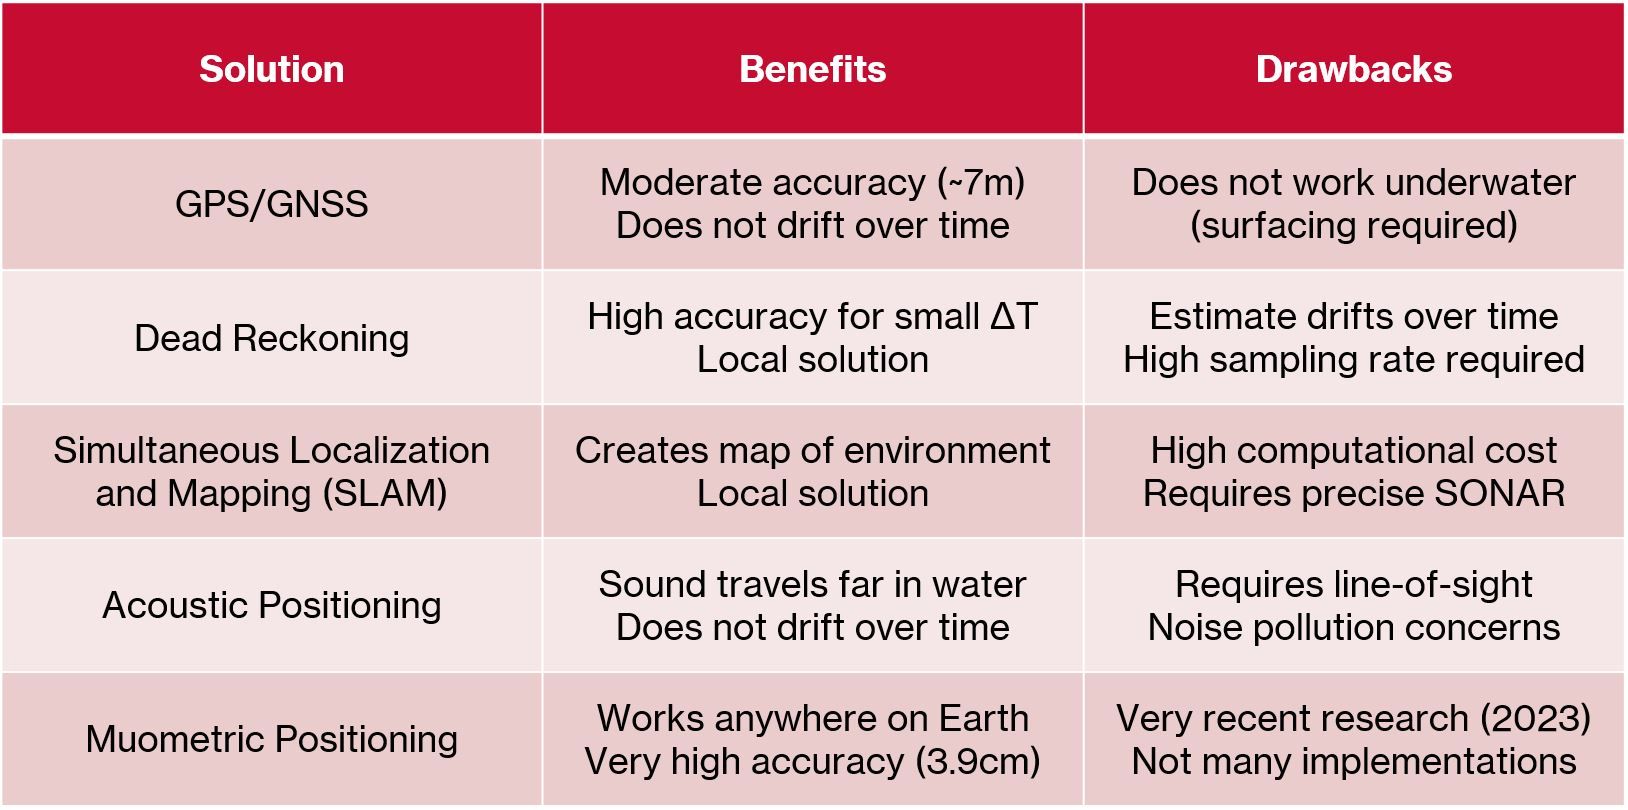
\includegraphics[width=\textwidth]{upstable}
	\captionfonts
	\caption{Common underwater positioning methods}
	\label{fig:upstable}
\end{figure}

GPS (which is a type of global navigation satellite system, or GNSS) is the most popular positioning method above-water and can be used to position AUVs when they surface. GPS uses a constellation of 31 satellites which constantly transmit their location and the time that the message was sent; from this information, a receiver can determine its position on Earth \cite{faagps}. As previously stated, GPS does not work underwater, so AUVs must come to the surface to get a new position estimate from the GPS.

Dead reckoning is a method for determining a change in position by integrating velocity and heading over time. Its history and working mechanisms are covered in detail in Section \ref{sec:4s5}. Dead reckoning can be very accurate over small periods of time with proper equipment, but the position estimate quickly accumulates error over time. Dead reckoning is a local solution, not requiring any external satellites or vehicles, but a purely dead reckoning-based navigation system is not feasible for most scenarios. A common low-cost, low-complexity implementation is to combine GPS and dead reckoning: get a GPS position estimate at the surface, then use dead reckoning while underwater. This implementation does mean that the position estimate gets worse over time, which can be detrimental in certain scenarios.

Simultaneous localization and mapping (SLAM) is a highly-complex navigation method. It uses SONAR equipment (or cameras) to collect data about the environment, creates a map of the local environment, and then localizes itself (determines its position) within that map. For AUVs used in seafloor mapping, it is a wonderful solution since the process requires constructing a map of the environment. Additionally, it only uses on-board equipment and sensors --- no satellites or buoys required. This means that it can only provide a position estimate within the local frame, so some other method of absolute positioning (like GPS) is required to know the position of the AUV in the global frame. This method comes with a high computational cost and requires expensive and precise equipment, but presents a unique solution to the positioning problem \cite{surveyurpn}.

Acoustic positioning is a method for determining the position of the AUV relative to a set of buoy-, seafloor-, or hull-mounted microphones. It essentially functions like an underwater GPS system, using sound waves instead of radio waves. This method does not drift over time like the previous two, but does require line-of-sight (line-of-sound?) to the underwater microphones. This method is the main focus of this thesis and is covered in depth in Chapter \ref{chap:3c}.

Finally, a brand-new underwater positioning method is muometric positioning, pioneered by Hiroyuki Tanaka. In this method, cosmic-ray muons (which bombard the Earth constantly) are detected at receiver stations, and the time-of-arrival between the receiver stations is used to determine the position of an object. Muons are capable of passing through most solid materials, meaning that the system can be used in buildings, underwater, or underground \cite{muons}. It is very new research, and is a field well-worth exploring!

\section{High-Level Overview} \label{sec:1s3}
For a single researcher, designing an acoustic positioning system and implementing it underwater is a massive task; for simplification, this system will be prototyped for above-water use. Figure \ref{fig:underwaterimp} shows how the proposed underwater system would function. A buoy with a GPS receiver is able to communicate with GPS satellites, so its position is known in the global frame. On the underside of the buoy, an acoustic transmitter sends out pulses of sound into the water beneath it. The AUV (whose position is desired) is below the buoy, within the cone of sound of the transmitter. Microphones on the body of the AUV record a pulse from the transmitter and use acoustic positioning methods to determine the location of the AUV relative to the buoy. The GPS coordinates of the buoy are encoded in the sound pulse. The AUV knows where it is relative to the buoy, and the GPS coordinates describe where the buoy is relative to the global frame; this information can be combined to give the position of the AUV in the global frame. Additionally, dead reckoning is used on the AUV to supplement the acoustic position estimates. These two estimates are combined using a Kalman filter to produce the best position estimate for the AUV in the global frame.

\begin{figure}[htbp]
	\centering
	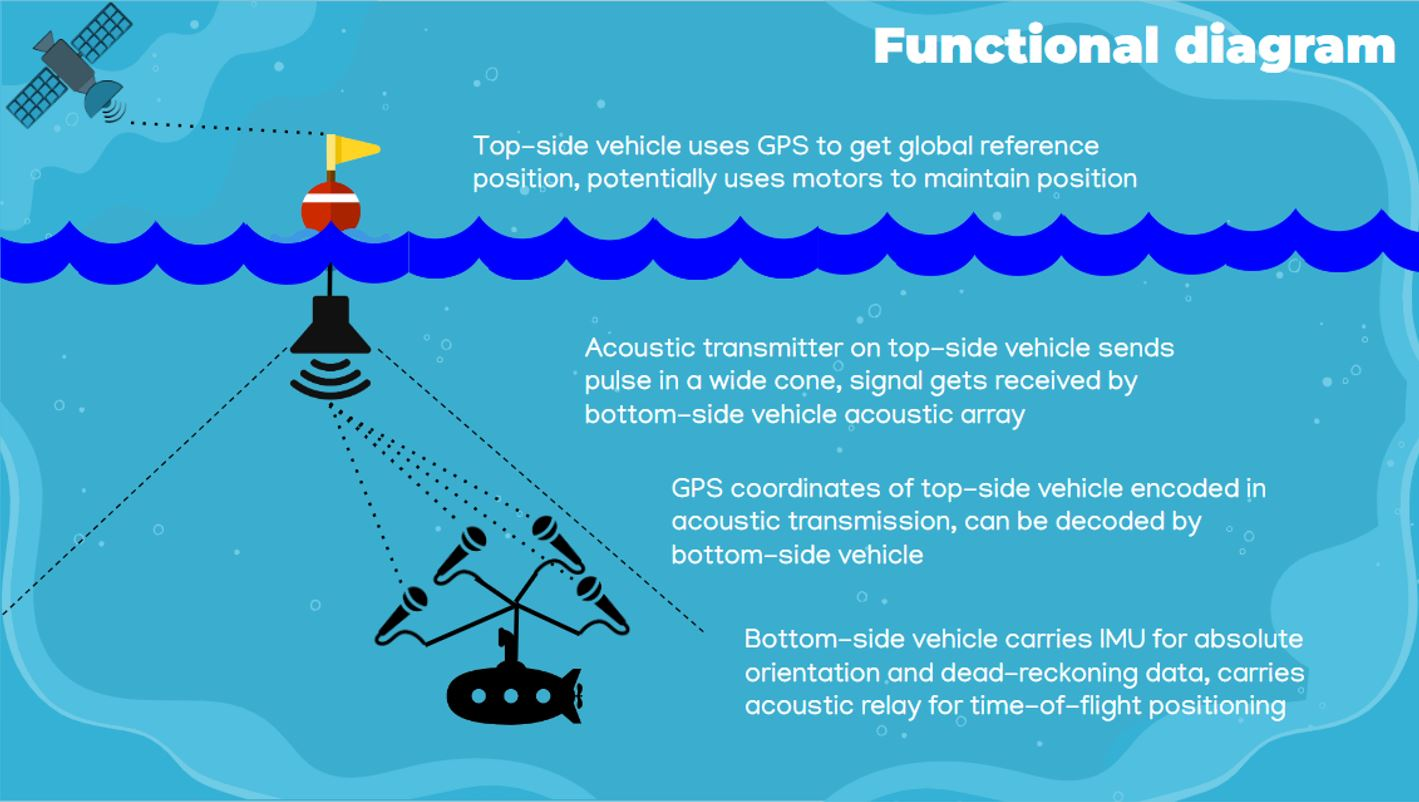
\includegraphics[width=\textwidth]{underwaterimp}
	\caption{Functional diagram for proposed underwater implementation}
	\label{fig:underwaterimp}
\end{figure}

The above-water prototype in this thesis is very similar to the proposed underwater implementation. To verify the accuracy of this system, a ground-truth positioning system is designed and fabricated; this system determines the true location of the microphone array (the above-water equivalent of the AUV). A relatively-novel actuator, a stacked hexapod platform, was used as the ground truth positioning system. The design process for the ground-truth positioning system is covered in Chapter \ref{chap:2c}.

The acoustic positioning system functions as follows: the transmitter sends out a pulse of sound, the microphones on the receiver array record the pulse, the time shift between the recordings is calculated, and the position of the transmitter relative to the receiver array is determined. This is combined with the true position of the transmitter (GPS coordinates sent over the acoustic pulse) to determine the position of the receiver array in the global frame. Chapter \ref{chap:3c} details this process.

The orientation of the receiver array / AUV must be known to transform the position estimate to the global frame. This implementation uses a Madgwick filter, a sensor fusion filter for obtaining orientation estimates using inertial measurement units (IMUs). This process, along with the implementation of a dead reckoning system, is covered in Chapter \ref{chap:4c}.

The acoustic position estimate and the dead reckoning change-in-position estimate are fused together using a Kalman filter, and this model is called the iSBL-SF algorithm; this process is detailed in Chapter \ref{chap:5c}, which includes an explanation of how Kalman filters work.

Finally, the system accuracy is tested and evaluated in Chapter \ref{chap:6c}, along with an extrapolation of the above-water results to the underwater regime. Chapter \ref{chap:7c} includes recommendations for improving upon the work presented in this thesis.






%-------------------------CHAPTER 2-------------------------





\chapter{Ground-Truth Positioning System} \label{chap:2c}
Testing the accuracy of the proposed positioning system algorithm requires knowing where the system truly is --- thus, a ground-truth positioning system is needed. This system should give the true position of the receiver array (with some uncertainty), and should be controllable and positionable to allow testing of different locations. 

This chapter details the design of the Fo-SHIP, the ground-truth positioning system for this thesis. First, the inspiration behind the design and previous works that the Fo-SHIP builds off of are discussed. The mechanical and electrical design are detailed, and the manufacturing and assembly are shown. Then, the software running the Fo-SHIP is documented. Lastly, the calibration, testing, and validation of the system are described.

\section{Design Inspiration and Previous Works} \label{sec:2s1}
The ground-truth positioning system for this thesis is modeled after a unique actuator henceforth known as a “stacked hexapod platform,” as first described in a publication from NASA Langley Research Center \cite{nasaSSPpaper}. In the paper, Balaban, Cooper, and Komendera constructed an actuator they called an “Assembler” made of multiple Stewart platforms that are vertically stacked upon each other. The mechanism is a novel attempt at creating a robotic system that can assemble structures in space, and was the only one of its kind prior to the development of this thesis (to the author's knowledge). A picture of their actuator is shown in Figure \ref{fig:nasassp} below.

\begin{figure}[htbp]
	\centering
	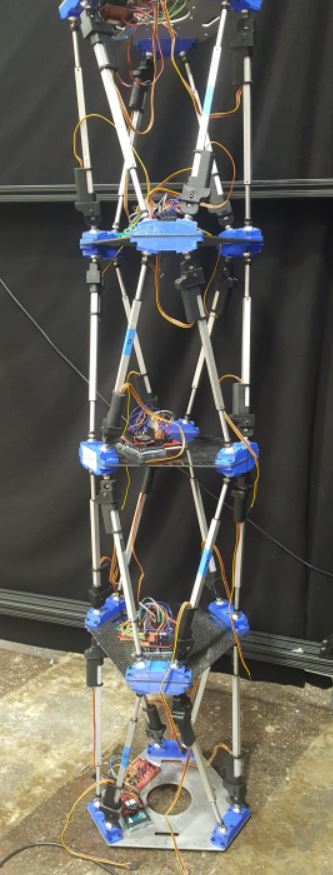
\includegraphics[width=0.5\textwidth]{nasassp}
	\caption{Stacked Stewart platform from Balaban, Cooper, and Komendera \cite{nasaSSPpaper}}
	\label{fig:nasassp}
\end{figure}

\subsection{Stewart Platform Origins} \label{ssec:2s1s1}
A Stewart platform, also known as a hexapod or Stewart-Gough platform, is a six degree-of-freedom (DOF) actuator invented in the mid-20th century. The true inventor of the platform is disputed. In 1954, Eric Gough, an automotive engineer, designed a hexapod platform to test different loading conditions on tires \cite{parallelorigins}. A picture of his platform is shown in Figure \ref{fig:goughplatform} below.

\begin{figure}[htbp]
	\centering
	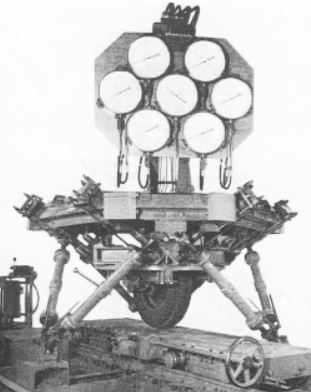
\includegraphics[width=0.5\textwidth]{goughplatform}
	\caption{Gough’s hexapod platform \cite{parallelorigins}}
	\label{fig:goughplatform}
\end{figure}

\vspace{1ex}
Eleven years later, D. Stewart (an engineer whose full first name appears to be unknown) published a paper proposing a platform with six degrees of freedom meant for use in flight simulators. In his paper, he noted correspondence with Gough \cite{stewartpaper}. An image of his proposed platform is shown in Figure \ref{fig:stewartOG} below.

\begin{figure}[htbp]
	\centering
	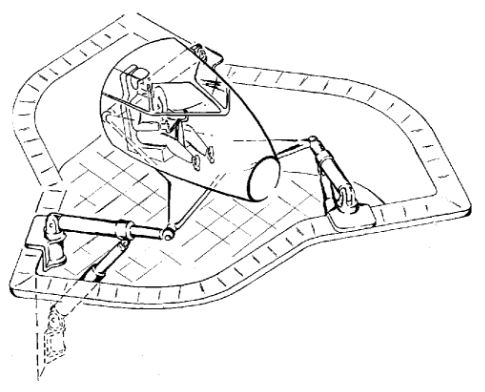
\includegraphics[width=0.5\textwidth]{stewartOG}
	\caption{Stewart’s hexapod platform \cite{stewartpaper}}
	\label{fig:stewartOG}
\end{figure}

Additionally, an engineer named Klaus Cappel independently developed a hexapod platform as a flight simulator for helicopter pilots and constructed a prototype in 1964 \cite{parallelorigins}. An image of Cappel’s platform is shown in Figure \ref{fig:cappelplatform}.

\begin{figure}[htbp]
	\centering
	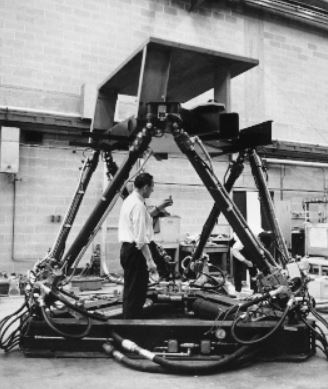
\includegraphics[width=0.5\textwidth]{cappelplatform}
	\caption{Cappel’s hexapod platform \cite{parallelorigins}}
	\label{fig:cappelplatform}
\end{figure}

Despite the independent creations of the platform, Stewart’s name has stuck. Though “Stewart platform” is the most common name of this type of mechanism, the mechanism in this thesis’s implementation will be primarily referred to as a “hexapod."

\subsection{Reinforcement Learning Research} \label{ssec:2s1s2}
As part of an Artificial Intelligence course taken in pursuit of this Master’s degree, a deep reinforcement learning agent was designed to control a stacked hexapod platform \cite{cscpaper}. For this implementation, a custom Gymnasium (a common deep reinforcement learning framework \cite{gymnasium}) environment was developed to represent the kinematics of a stacked hexapod platform. A visualization of the environment is shown in Figure \ref{fig:deepRL} below.

\begin{figure}[htbp]
	\centering
	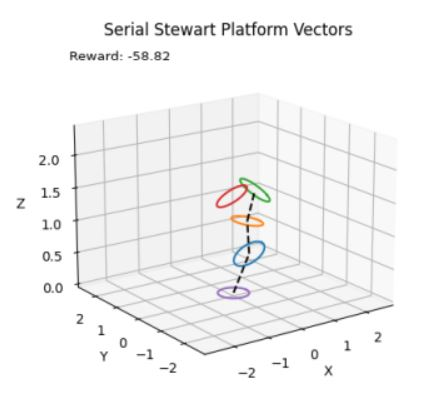
\includegraphics[width=0.5\textwidth]{deepRL}
	\caption{Custom stacked hexapod platform Gymnasium environment \cite{cscpaper}}
	\label{fig:deepRL}
\end{figure}

The location and orientation of a single hexapod platform is dependent on the platform directly beneath it. Two vectors are used per platform: a position vector describes the distance between the centers of the top and bottom of a platform, and an orientation vector describes the vector normal to the surface of the top of the platform. This is a simplified implementation of a hexapod platform; normally, they are described by the six actuators that connect the base and the top. However, the simplified implementation was much easier to work with for a first attempt at deep reinforcement learning. Additionally, the simplified implementation can be related to the true implementation (using six actuators) using kinematics, so the model still moves as a “true” hexapod platform would.

The reinforcement learning attempt ultimately did not succeed due to errors in the Gymnasium implementation (which were identified months after the initial attempt). However, this first attempt at creating a stacked hexapod platform was the inspiration behind the ground-truth positioning system for this thesis. Future plans are to train a deep reinforcement learning agent to control the platform built for this thesis, using an improved Gymnasium environment and interfacing with the real-world system.

\subsection{Inverse Kinematics of a Single Hexapod Platform} \label{ssec:2s1s3}
Much of the inverse kinematics work for this actuator was developed by previous authors. Notably, a paper by an unknown author from the Wokingham U3A Math Group details an inverse kinematics solution for a hexapod platform controlled by six rotary servos \cite{wokingham}. An art installation named “memememe” improved upon this solution and implemented the design into a single hexapod platform for controlling the motion of a smartphone attached to the end effector \cite{meme}. Lastly, an open-source implementation of a single hexapod platform using an ESP32 microcontroller was posted online by Nicolas Jeanmonod \cite{nicdoc} \cite{nichub}. This thesis has modified Jeanmonod’s implementation to work with a stacked hexapod platform and some new features and functions were added, but his work is the backbone of the hexapod platform controller. The details of the inverse kinematics of the platform will be described later in Section \ref{ssec:2s5s5}, along with their code implementation.

\subsection{Consideration of Alternative Systems} \label{ssec:2s1s4}
The stacked hexapod platform was one of many contenders for the ground-truth positioning system. The requirements for the ground-truth position system were:

\begin{itemize}[noitemsep,topsep=0pt]
	\item Six degrees of freedom --- translation and rotation about XYZ axes
	\item Low cost --- this thesis is not funded through grants or external sources
	\item Large range of motion --- at least capable of ±0.5m along some translational axis and ±45° about some rotational axis
	\item Acceptable accuracy --- true position must be within ±1cm of setpoint
\end{itemize}

\vspace{2ex}
\noindent The actuators considered were:

\begin{itemize}[noitemsep,topsep=0pt]
	\item Cartesian/gantry robot --- a robot constructed from linear actuators (similar to a 3D printer) and a rotating end effector
	\item Articulated arm robot --- a robot constructed from rotary actuators (similar to most industrial robotic arms)
	\item Stacked hexapod platform --- a robot constructed from stacked hexapod platforms
	\item Cable-driven robot --- a robot with a large frame and multiple (6-8) cable-driven actuators that move an end effector in the center of the frame
\end{itemize}

\vspace{2ex}
\noindent The evaluation criteria were:

\begin{itemize}[noitemsep,topsep=0pt,]
	\item Accuracy --- is the system capable of acceptable accuracy and repeatability? Higher accuracy is better
	\item Cost --- is the actuator low-cost to design and manufacture? Lower cost is better
	\item Manufacturability --- how feasible is it to make the parts required to the necessary tolerances? Easier manufacturability is better
	\item Research potential --- is it a novel system? More novel and less widely used is better
	\item Relative size --- how large is the system compared to its range of motion? Smaller is better
	\item Complexity --- how many moving parts does the system have? Lower complexity is better
\end{itemize}

\noindent A Pugh matrix below shows the consideration process. Ultimately, the stacked hexapod platform was chosen due to its low cost, high research potential, and manufacturability. 

\begin{table}[htbp]
	\centering
	\caption{Pugh matrix for ground-truth positioning system actuator}
	\label{tab:pughmatrix}
	\begin{tabular}{|c|c|c|c|c|c|}
		\hline
		\makecell{Criteria} & \makecell{Weight} & \makecell{Cartesian\\robot} & \makecell{Articulated\\robot} & \makecell{Stacked\\hexapod\\platform} & \makecell{Cable-\\-driven\\robot} \\
		\hline
		Accuracy & 3 & Datum & - & - & - \\
		\hline
		Cost & 5 & Datum & + & + & + \\
		\hline
		Manufacturability & 2 & Datum & S & + & - \\
		\hline
		Research potential & 4 & Datum & S & + & + \\
		\hline
		Relative size & 3 & Datum & + & + & S \\
		\hline
		Complexity & 1 & Datum & + & - & - \\
		\hline
		\multicolumn{2}{|c|}{Weighted Sums} & 0 & 6 & 10 & 3 \\
		\hline
	\end{tabular}
\end{table}

The chosen system has been named the “Four-Stacked Hexapod Isometric Platform,” abbreviated as Fo-SHIP. The system is four equally-sized (isometric) hexapod platforms stacked upon each other. As an added bonus, the pronunciation of Fo-SHIP sounds like “faux ship,” which is exactly what this positioner is: a fake version of the submarine that the acoustic positioning system will be eventually deployed on.

\section{Mechanical Design} \label{sec:2s2}
The mechanical design of the Fo-SHIP is inspired by Jeanmonod’s implementation \cite{nicdoc}. His design, shown below, uses six rotary servos sandwiched between two hexagonal plates as the base, and a single hexagonal plate as the top / end effector. Ball joints are used to connect threaded rods to the servo horns and the end effector plate. The top hexagonal plate is 3D printed and uses heat-set threaded inserts to secure the ball joints, while the base plates appear to be made from composite board material. His design is fully documented and a parts list is available on the project’s GitHub page \cite{nichub}. A CAD rendering and physical model of Jeanmonod's implementation can be seen in Figures \ref{fig:nicplatform} and \ref{fig:nicplatform2}, respectively. 

\begin{figure}[htbp]
	\centering
	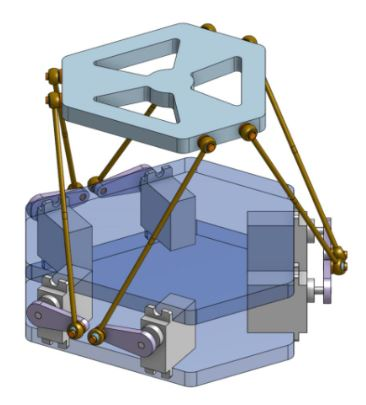
\includegraphics[width=0.5\textwidth]{nicplatform}
	\caption{Jeanmonod’s implementation of a single hexapod platform, CAD model \cite{nichub}}
	\label{fig:nicplatform}
\end{figure}

\begin{figure}[htbp]
	\centering
	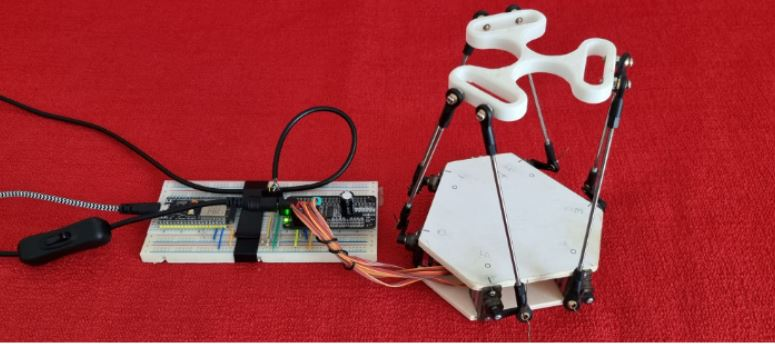
\includegraphics[width=\textwidth]{nicplatform2}
	\caption{Jeanmonod’s implementation of a single hexapod platform, physical model \cite{nicdoc}}
	\label{fig:nicplatform2}
\end{figure}

Jeanmonod's implementation would need to be modified to fit the goals of this thesis. The top and bottom platforms are different sizes, which would not work for a stacked hexapod platform where each level is of uniform size. Making each level the same size makes manufacturing and design much easier; however, the load on each level is not uniform, which means that the bottom-most level experiences much more force and wear than the top-most level. In future implementations of stacked hexapod platforms, a cascading design (where the bottom-most level is larger and has more powerful motors, and the size/weight of each platform decreases as a function of the platform's location in the stack) would be recommended.

The implementation for this thesis is shown below. It uses a common plate design which can be modified for the needs of each individual platform. The base plate of the first platform, Figure \ref{fig:firstbase}, has three through holes for \sfrac{3}{8}”-16 bolts to attach the Fo-SHIP to a wooden base. The base plates of the second and fourth platform, Figure \ref{fig:secondbase}, have mounting slots for a PCA9685 servo driver and an MPU6050 IMU (details in Section \ref{ssec:2s5s2}). The base plate of the third platform, Figure \ref{fig:thirdbase}, has a mounting slot for the MPU6050 only. The middle plate of each platform, Figure \ref{fig:midbase}, has holes to allow servo wires to pass through (this plate sits on top of the servos). The top / end effector plate, Figure \ref{fig:endplate}, has mounting holes to attach the iSBL array adapter. Figure \ref{fig:secondplatstack} shows the spacing between plates for the second platform. All plates were modeled using Solidworks\textsuperscript{\textregistered}\xspace.

\begin{figure}[htbp]
	\centering
	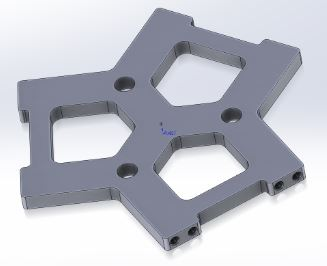
\includegraphics[width=0.5\textwidth]{firstbase}
	\caption{First platform base plate}
	\label{fig:firstbase}
\end{figure}

\begin{figure}[htbp]
	\centering
	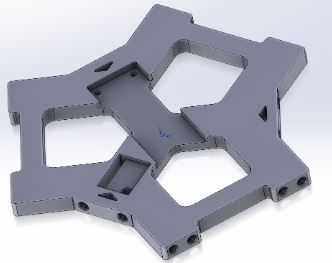
\includegraphics[width=0.5\textwidth]{secondbase}
	\caption{Second and fourth platform base plate}
	\label{fig:secondbase}
\end{figure}

\begin{figure}[htbp]
	\centering
	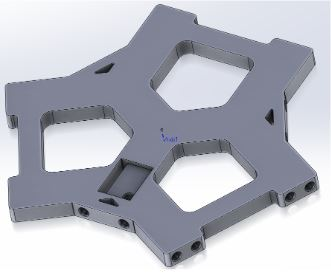
\includegraphics[width=0.5\textwidth]{thirdbase}
	\caption{Third platform base plate}
	\label{fig:thirdbase}
\end{figure}

\begin{figure}[htbp]
	\centering
	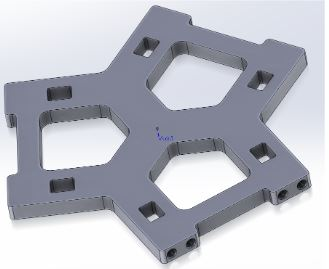
\includegraphics[width=0.5\textwidth]{midbase}
	\caption{Middle plate for all platforms}
	\label{fig:midbase}
\end{figure}

\begin{figure}[htbp]
	\centering
	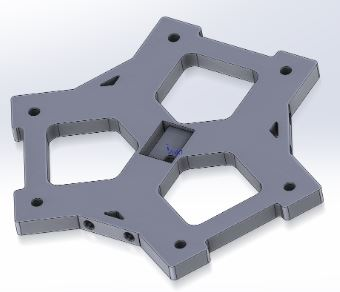
\includegraphics[width=0.5\textwidth]{endplate}
	\caption{End effector plate}
	\label{fig:endplate}
\end{figure}

\begin{figure}[htbp]
	\centering
	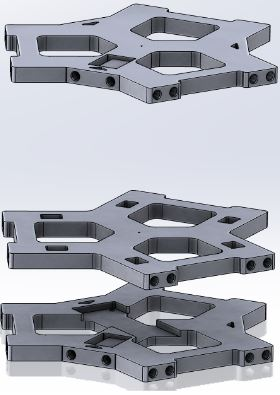
\includegraphics[width=0.5\textwidth]{secondplatstack}
	\caption{Spacing of plates for second platform}
	\label{fig:secondplatstack}
\end{figure}

The plates were printed in the Cal Poly Mustang ‘60 Machine Shop on Prusa Mk.3 FDM printers using PETG filament. PETG was chosen due to its strength, durability, non-brittle nature, and heat resistance when compared to materials like PLA \cite{plapetg}. Figure \ref{fig:rawpca} shows one of the printed base plates with a PCA9685 servo driver resting in its mounting slot.

\begin{figure}[htbp]
	\centering
	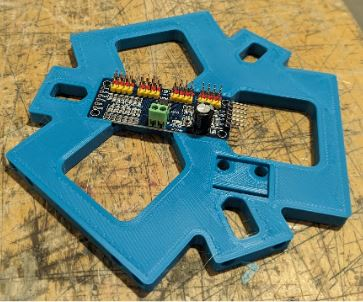
\includegraphics[width=0.5\textwidth]{rawpca}
	\caption{Printed base plate with PCA9685 servo driver}
	\label{fig:rawpca}
\end{figure}

A bill of materials for all components of the Fo-SHIP is shown in Table \ref{tab:bomfoship}. Note that some equipment used for fabrication, such as soldering irons and 3D printers, is essential to the build and is not factored into the bill of materials.

\begin{table}[htbp]
	\centering
	\caption{Bill of materials for Fo-SHIP}
	\label{tab:bomfoship}
	\begin{tabular}{|c|c|c|c|}
		\hline
		Item & Quantity & Price (ea) & Vendor \\
		\hline
		Blue PETG filament, 1kg & 1 & \$25 & Amazon \\
		\hline
		MG996R servo motors, 6 pieces & 4 & \$27 & Amazon \\
		\hline
		Metal ball joint, M3, 12 pieces & 4 & \$12 & Amazon \\
		\hline
		Threaded inserts, M3, 120 pieces & 2 & \$7 & Amazon \\
		\hline
		Threaded rods, M3, 100mm, 12 pieces & 2 & \$6 & Amazon \\
		\hline
		Aluminum servo horns, M3, 10 pieces & 3 & \$14 & Amazon \\
		\hline
		M3x8 socket head cap screws, 100 pieces & 1 & \$8 & Amazon \\
		\hline
		M3x5 socket head cap screws, 50 pieces & 2 & \$5 & Amazon \\
		\hline
		M3 hexagonal nuts, 100 pieces & 1 & \$10 & Ace Hardware \\
		\hline
		M3x20 phillips head screws, 25 pieces & 1 & \$10 & Ace Hardware \\
		\hline
		3/8”-16 hexagonal bolt & 3 & \$1 & Ace Hardware \\
		\hline
		3/8”-16 hexagonal nut & 3 & \$1 & Ace Hardware \\
		\hline
		M2x4 screw, 5 pieces & 1 & \$2 & Ace Hardware \\
		\hline
		M2 hexagonal nut, 5 pieces & 1 & \$2 & Ace Hardware \\
		\hline
		ESP32-WROOM microcontroller & 1 & \$10 & Amazon \\
		\hline
		PCA9685 servo driver board, 2 pieces & 1 & \$14 & Amazon \\
		\hline
		MPU6050 IMU, 3 pieces & 2 & \$10 & Amazon \\
		\hline
		DC variable power supply, 0-30V, 0-30A & 1 & \$50 & Amazon \\
		\hline
		MPU6050 IMU, 3 pieces & 2 & \$10 & Amazon \\
		\hline
		Jumper wires, assorted & 2 & \$7 & Amazon \\
		\hline
		Solderless breadboard pack & 1 & \$8 & Amazon \\
		\hline
		24-gauge wire, assorted colors, 30 feet each & 1 & \$15 & Amazon \\
		\hline
		Scrap wood boards for base of platform & 2 & \$0 & Machine shop \\
		\hline
		\multicolumn{2}{|c|}{Total Cost} & \$292 &  \\
		\hline
	\end{tabular}
\end{table}

\vspace{2ex}
Lastly, Jeanmonod’s code implementation uses the dimensions of the platform to compute the inverse kinematics model. Certain parameters are used to perform these calculations; the values used for this thesis’s implementation (based on the models above) are located in Table \ref{tab:foshipparams}. A diagram of the parameters can be seen below in Figure \ref{fig:hexparams}.

\begin{table}[!htbp]
	\ssp
	\centering
	\caption{Parameters for hexapod platform code implementation}
	\label{tab:foshipparams}
	\renewcommand{\arraystretch}{1.2}
	\begin{tabular}{|>{\centering\arraybackslash}m{3cm}|>{\centering\arraybackslash}m{3cm}|>{\centering\arraybackslash}m{1.5cm}|>{\centering\arraybackslash}m{5cm}|}
		\hline
		\makecell{Parameter name} & \makecell{Measurement} & Units & \makecell{Determination method} \\
		\hline
		ROD\_LENGTH & 106.0 & mm & Measured six assembled threaded rods with ball joints attached, took average, then assembled all other rods and set to that uniform length \\
		\hline
		Z\_HOME & 100 & mm & Personal preference --- servo horns are horizontal at 90mm, but setting to 100mm gives greater range-of-motion for angular displacement \\
		\hline
		ARM\_LENGTH & 24.0 & mm & Measured six aluminum servo horns with calipers, took average \\
		\hline
		THETA\_P & 50.02 & deg & Computed from CAD model, verified using calipers and trigonometry on printed parts \\
		\hline
		THETA\_B & 20.53 & deg & Computed from CAD model, verified using calipers and trigonometry on printed parts \\
		\hline
		THETA\_S & 120 & deg & Computed from CAD model, verified using calipers and trigonometry on printed parts \\
		\hline
		P\_RAD & 57.73 & mm & Computed from CAD model, verified using calipers on assembled platform, took average of three readings \\
		\hline
		B\_RAD & 82.7 & mm & Computed from CAD model, verified using calipers on assembled platform, took average of three readings \\
		\hline
	\end{tabular}
\end{table}

\begin{figure}[!htbp]
	\centering
	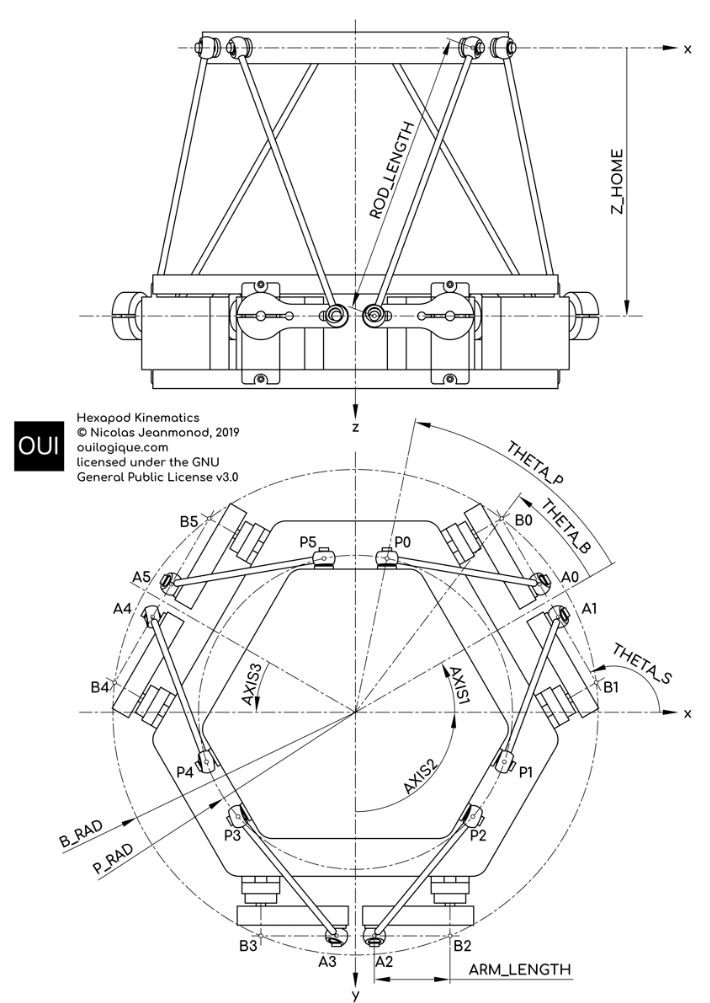
\includegraphics[width=0.9\textwidth]{hexparams}
	\caption{Parameters for hexapod platform in Jeanmonod’s code implementation \cite{nichub}}
	\label{fig:hexparams}
\end{figure}

\vspace{10pt}
\section{Electrical Design} \label{sec:2s3}
The electrical wiring and design of the Fo-SHIP is relatively straightforward --- it consists of an ESP32 microcontroller communicating with two PCA9685 servo drivers and five MPU6050 IMUs. The PCA9685 is a servo controller board that communicates with a microcontroller (or other controller) over I\textsuperscript{2}C, a common electronics protocol. It has 16 channels that use standard hobby servo motor wiring (ground / 5V / PWM); by sending the correct message over I\textsuperscript{2}C, the microcontroller can control up to 16 servo motors, LEDs, or anything that takes in a PWM signal \cite{pca9685datasheet}.

PWM, or pulse width modulation, is a technique for modulating the width of an electrical pulse. For servo motors, a common protocol is to divide pulses into 20ms periods and set the output to “high” for a certain amount of time, depending on the angle desired. Figure 16 shows a common configuration for hobby servo motors. The specifics of how the instructions for a certain pulse width are sent from the microcontroller to the PCA9685 are explained in Section \ref{sec:2s5}.

\begin{figure}[htbp]
	\centering
	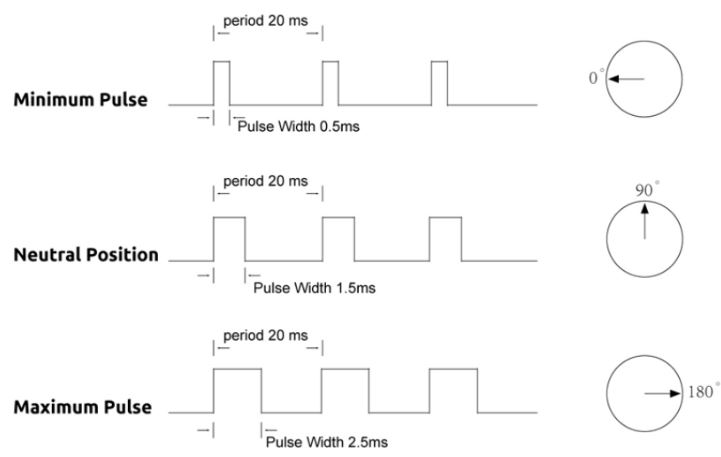
\includegraphics[width=0.9\textwidth]{servotiming}
	\caption{Hobby servo motor PWM timing \cite{servos}}
	\label{fig:servotiming}
\end{figure}

The MPU6050s also communicate over the same I\textsuperscript{2}C line. Each MPU6050 reads linear acceleration and angular velocity about three axes (XYZ). There is one MPU6050 attached to the wooden base of the Fo-SHIP, and one attached to the top of each hexapod platform. When the Fo-SHIP is at rest, the acceleration values can be read and converted to a 3D orientation. Using this data, any “slop” in the system is accounted for --- if the Fo-SHIP’s end effector is set to 15° about the X-axis, the true orientation for each hexapod platform can be measured (and it can be confirmed if the end effector is actually oriented at 15°). The specifics of how data is sent between the MPU6050s and the ESP32, how the accelerometer data is converted to orientation, and how the true orientation can be used to correct the forward kinematics model of the Fo-SHIP are discussed in Section \ref{sec:2s5}. 

For I\textsuperscript{2}C, all that is needed is four wires: ground, power, SDA (data), and SCL (clock). For two (or more) devices that are communicating over I\textsuperscript{2}C, all devices share the same line for each of the four wires, and a pullup resistor is added to the SDA and SCL lines. Figure \ref{fig:i2cwiring} shows a common wiring schematic for I\textsuperscript{2}C communication.

\begin{figure}[htbp]
	\centering
	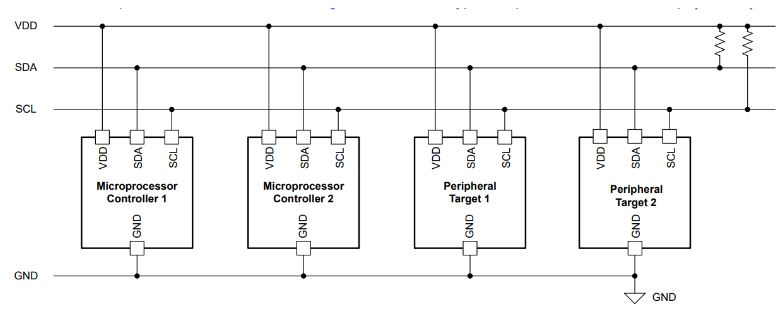
\includegraphics[width=0.9\textwidth]{i2cwiring}
	\caption{Typical I\textsuperscript{2}C wiring \cite{tiI2C}}
	\label{fig:i2cwiring}
\end{figure}

The ESP32, PCA9685s, and MPU6050s are all connected to the same I\textsuperscript{2}C bus. Each MPU6050 has an AD0 pin that must be pulled low (to ground) to choose which IMU to read from. Additionally, the ESP32 is connected via USB to a laptop, providing logic power and facilitating data transfer via UART. There is a button connected to one of the ESP32 general purpose input-output (GPIO) pins for user interaction and to begin data collection. The ESP32 is also connected to an STM32 microcontroller via a serial bus (RX/TX). Lastly, the PCA9685s have an additional power input to provide high-current power to the 24 servos of the Fo-SHIP. A wiring diagram for the Fo-SHIP can be seen in Figure \ref{fig:foshipwiring}.

\begin{figure}[htbp]
	\centering
	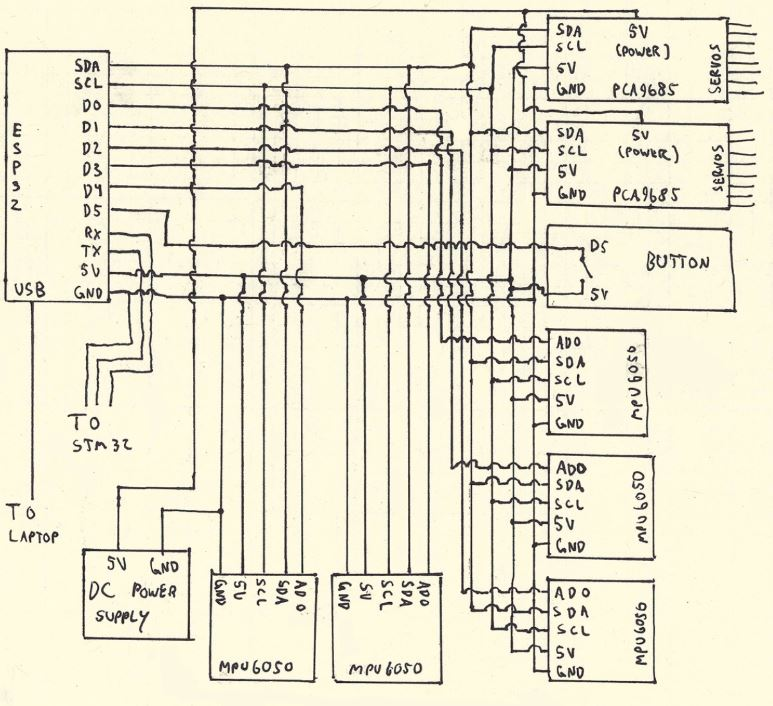
\includegraphics[width=0.9\textwidth]{foshipwiring}
	\caption{Fo-SHIP wiring diagram}
	\label{fig:foshipwiring}
\end{figure}

\section{Manufacturing and Assembly} \label{sec:2s4}
As stated in Section \ref{sec:2s2}, the plates of the Fo-SHIP were printed in the Cal Poly Mustang ‘60 Machine Shop over the course of two weeks. M3 threaded inserts were heat-set into blind and through holes in the plates using a soldering iron. Note that the mounting slots for the PCA9685 and MPU6050 have through holes for heat-set inserts as well.

A wooden base was manufactured from two boards: one on the bottom that has a large circular cutout, and another on top that has through holes for the mounting bolts. The bottom board is necessary to provide an offset between the ground and the mounting bolts and nuts. The wooden base can be seen in Figure \ref{fig:woodenbase}.

\begin{figure}[htbp]
	\centering
	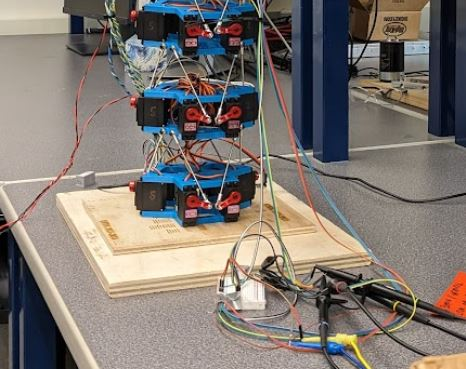
\includegraphics[width=0.7\textwidth]{woodenbase}
	\caption{Wooden base of Fo-SHIP}
	\label{fig:woodenbase}
\end{figure}

The Fo-SHIP was assembled one level at a time, starting with the bottom platform. The servos were mounted between the base and middle plate of the first platform, loosely secured using M3x5 socket head cap screws. The servos were adjusted to be parallel with the edges of the plates, and the screws were tightened in a star pattern to avoid uneven clamping forces and misalignments. The servos were then powered and set to an angle of 90° (horizontal). Aluminum servo horns were placed on the servo outputs; adjacent horns were placed to be pointed towards each other as shown in Figure \ref{fig:firsttwoplat}. The horns were attached using screws to the servo output and were further secured via small, off-center screws that clamp the body of the horn around the servo output.

The threaded rod linkages were assembled by screwing on threaded ball joint connectors at both ends, turning each connector an equal amount to ensure equal thread penetration. The length between the centers of each ball joint bearing was measured, and the ball joints were adjusted until the length was 106mm ± 1mm. For each platform, six linkages were gathered and each was attached to the inside of a servo horn at the furthest threaded hole. An M3x20 screw was placed through the ball joint bearing and screwed into the servo horn. Once tightened, an M3 nut was secured to the end of the M3x20 screw and torqued to prevent the connection from loosening.

A second platform was assembled as described in the previous paragraph up until after the servo horns were secured. Then, both platforms were laid horizontally on a table and the linkages from the first platform were secured to the corresponding threaded inserts on the base of the second platform using M3x8 screws. Care was taken to avoid over-torquing any threaded inserts, since they are secured only by melted plastic. 

The above process was repeated until four platforms had been assembled. At this point, the end effector plate was attached to the top-most platform.

\begin{figure}[htbp]
	\centering
	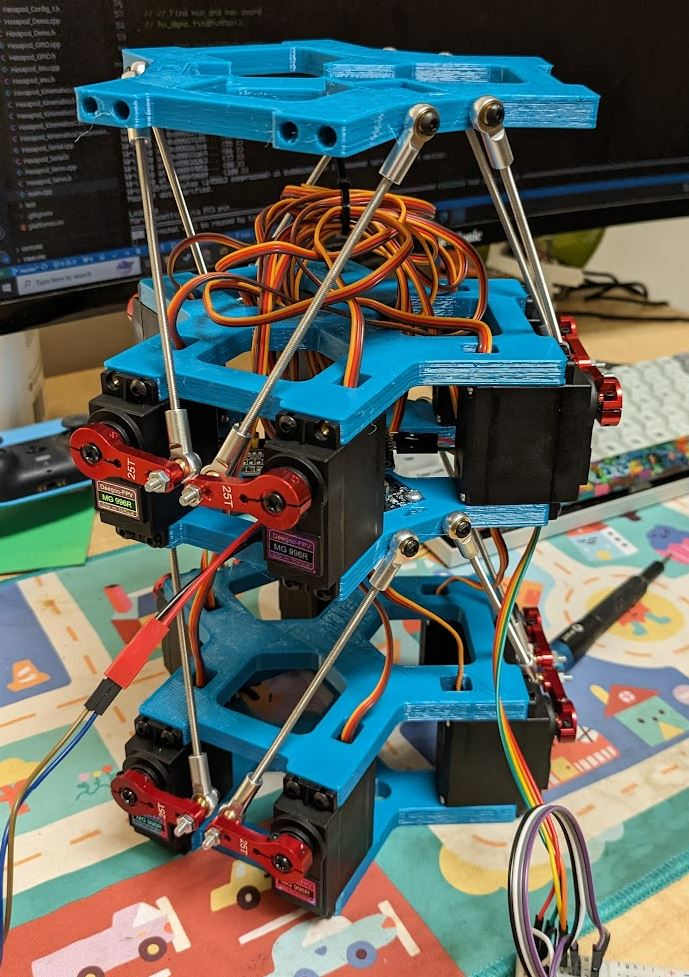
\includegraphics[width=0.9\textwidth]{firsttwoplat}
	\caption{Assembled Fo-SHIP, first two layers}
	\label{fig:firsttwoplat}
\end{figure}

Once all platforms were assembled, an MPU6050 was attached to the base of each platform (besides the first level), to the end effector plate, and to the wooden base. The MPU6050s were secured using M3x5 screws and care was taken to avoid over-torquing the screws and deforming the plastic beneath, which would result in an altered angle reading from the IMUs. Then, the PCA9685 boards were attached to the base of the second and fourth platform and secured with M2x4 screws and M2 nuts. Once secured, the servo wires were attached to the PCA9685 boards in a clockwise pattern. A number was written on each servo’s body to note which pins it connects to on its corresponding PCA9685 board. Wires were added to each MPU6050 and PCA9685 in accordance with the wiring diagram in Section \ref{sec:2s3} and were connected to a breadboard that held the ESP32 microcontroller. 

The breadboard and the button included in the wiring diagram were secured to the wooden base with adhesive. Loose wires were joined using cable ties, and hot glue was used to insulate electrical connections and prevent wires from dislodging from the breadboard. The fully-assembled Fo-SHIP with all platforms and wiring can be seen in Figure \ref{fig:fullplats} below.

\begin{figure}[htbp]
	\centering
	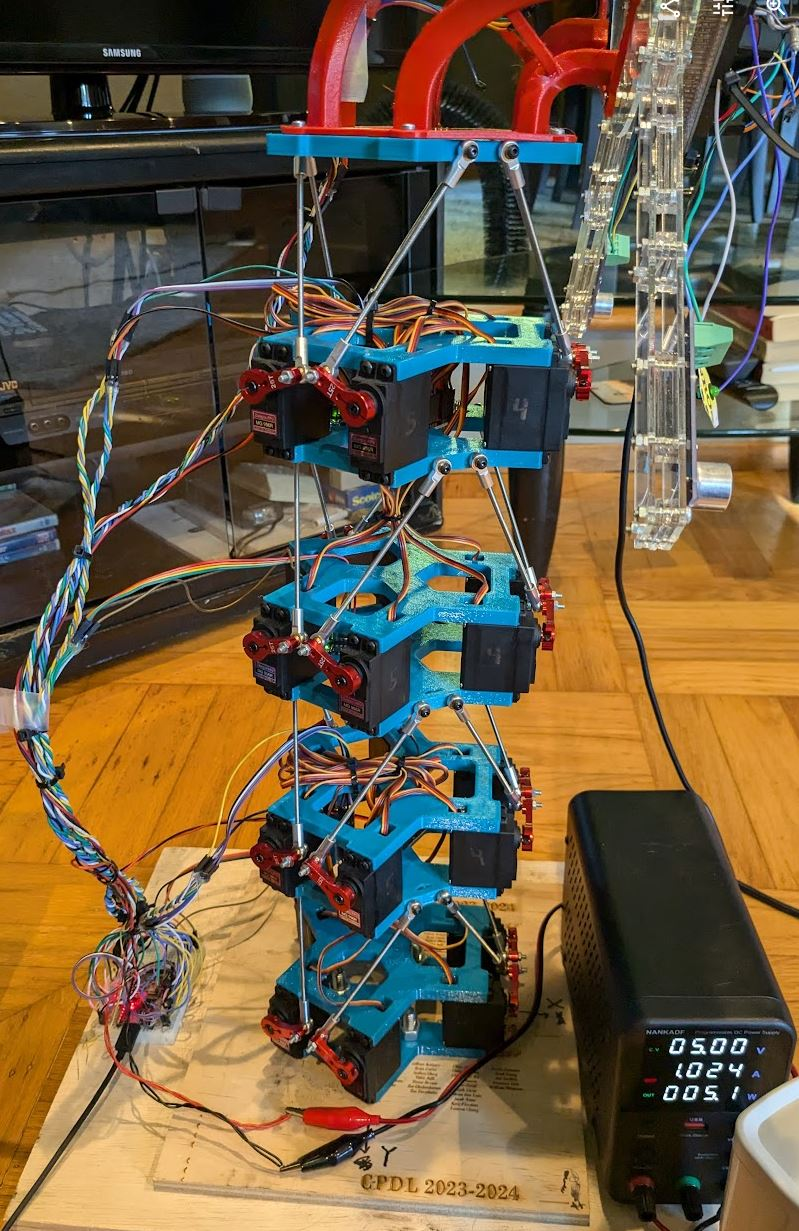
\includegraphics[width=0.8\textwidth]{fullplats}
	\caption{Fully-assembled Fo-SHIP body}
	\label{fig:fullplats}
\end{figure}

\vspace{10pt}
\section{Software Design} \label{sec:2s5}
This section will be broken down into six subsections. The first will show custom structs used for the code and the configuration / parameters of each platform of the Fo-SHIP. The second will discuss the MPU6050 failures and how a workaround was implemented. The third will discuss the main program initialization and main loop, and will include a finite-state machine representation of the code. The fourth will detail the forward kinematics calculations for the multi-platform configuration, focusing on the big-picture of how one platform affects the next. The fifth will derive the inverse kinematics algorithm used to calculate servo angles for a single platform’s setpoint. The last will explain some demonstration functions that show the full range-of-motion of the Fo-SHIP.

As stated previously, the majority of this code is built off of Nicolas Jeanmonod’s implementation on GitHub \cite{nichub}, and the Fo-SHIP would not be functional without his contributions.

\subsection{Custom Structs and Hexapod Configuration} \label{ssec:2s5s1}
The Fo-SHIP uses a few custom structs for its data processing. First, \verb|calibration_t| is a struct used for saving the gains and offsets of each individual servo. 

\begin{lstlisting}[language=C++]
typedef struct
{
	double gain;
	int offset;
} calibration_t;
\end{lstlisting}

Next, \verb|angle_t| is a struct used for saving information about each servo’s angle in a variety of units: radians, degrees, microseconds (for PWM timing) and the PWM value (int from 0 to 4096).

\begin{lstlisting}[language=C++]
typedef struct
{
	double rad;			// Servo angle in radian.
	double deg;			// Servo angle in degrees.
	int us;				// Servo angle in us (PWM).
	uint16_t pwm_us; 	// Servo angle in range 0 to 4096 (PWM).
	double debug;		// Used for debug.
} angle_t;
\end{lstlisting}

Lastly, \verb|platform_t| is the most common struct used in the main program code. It defines the setpoint for a single platform with six coordinates, one for each major axis: (X, Y, Z, A, B, C), where A is roll about the X-axis, B is pitch about the Y-axis, and C is yaw about the Z-axis.

\begin{lstlisting}[language=C++]
typedef struct
{
	double hx_x; // Surge, translation along X axis (mm)
	double hx_y; // Sway, translation along Y axis (mm)
	double hx_z; // Heave, translation along Z axis (mm)
	double hx_a; // Roll, rotation around X axis (rad)
	double hx_b; // Pitch, rotation around Y axis (rad)
	double hx_c; // Yaw, rotation around Z axis (rad)
} platform_t;
\end{lstlisting}

Many configuration parameters are stored in \verb|Hexapod_Config1.h|. These include the parameters in Table \ref{tab:foshipparams}, as well as offset values for each servo, the full range of a servo described with a pulse width timing, minimum and maximum values for each axis of motion, and the orientation of each servo relative to the coordinate system.

\subsection{MPU6050 Failure and Workaround} \label{ssec:2s5s2}
After fully assembling the Fo-SHIP, it was discovered that only one out of the six MPU6050s purchased from Amazon was functional. Due to a limited budget and limited time (and after much testing of the MPU6050s to determine if they were truly faulty or if it was a code issue, which it was not), it was decided to forgo using any of the MPU6050s for orientation correction. However, the amount of slop in the Fo-SHIP’s many platforms required some sort of orientation correction for the forward kinematics calculations to be accurate. 

Thankfully, the iSBL receiver array has a high-quality (and functional) IMU which outputs the orientation of the end effector, which will be discussed more in Chapter \ref{chap:4c}. As a workaround, at the time of processing an acoustic measurement, the current orientation of the end effector is sent over UART from the STM32 to the ESP32. This orientation is assumed to be the true orientation of the end effector (top-most platform’s top plate). Assuming that the amount of slop in the system is uniform for each platform (and assuming that each platform is set to the same setpoint), the true orientation of a single platform relative to the one beneath it can be estimated as shown:

\begin{lstlisting}[language=C++]
modPos = currentPos;
modPos.hx_a = radians(stm_roll/4);
modPos.hx_b = radians(stm_pitch/4);
modPos.hx_c = radians(stm_yaw/4);
getEndEffectorCoords(&modPos, &modPos, &modPos, &modPos, false);
\end{lstlisting}

While this may seem like a large simplification, it reduces the inaccuracy of the Fo-SHIP’s position estimate by over 50\%. 

The original implementation for the MPU6050s is still in the code, and is not currently being used. The workflow for extracting the angle of each platform relative to the one beneath it using the MPU6050s is shown below. This workflow is for a single MPU6050 and is repeated for each platform's IMU:

\begin{itemize}[noitemsep,topsep=0pt]
	\item Take a number of readings from the MPU6050’s accelerometer, communicating over I\textsuperscript{2}C, and take the average to reject noise
	\item Convert the acceleration data into Euler angles (absolute orientation)
	\item Convert the absolute Euler angles into a rotation matrix
	\item Take the transpose of this matrix
	\item Multiply the rotation matrix for this platform by the transpose of the rotation matrix of the platform beneath it to get the relative orientation rotation matrix for this platform
	\item Extract the relative Euler angles from the relative orientation rotation matrix
	\item Save these Euler angles as the relative orientation of each platform
\end{itemize}

\noindent In the \verb|main.cpp| file, see these functions for more details:

\begin{itemize}[noitemsep,topsep=0pt]
	\item \verb|void readMPU(int IMU_NUM, int num_avgs);|
	\item \verb|void getEulerFromMPU(float *IMU_AccelData, float *IMU_Angles);|
	\item \verb|void getRotMatFromEuler(float *IMU_Angles, float *IMU_RotMat);|
	\item \verb|void getEulerFromRotMat(float *IMU_RotMat, float *IMU_Angles);|
	\item \verb|void multiply3x3Matrices(float *matA, float *matB, float|\\ \verb|*result);|
	\item \verb|void transposeMatrix(float *mat, float *result);|
	\item \verb|void multiply3x3MatrixVector(float *mat, float *vec, float|\\ \verb|*result);|
\end{itemize}

\subsection{Main Program} \label{ssec:2s5s3}
The main program in \verb|main.cpp| does a few things: it starts and maintains a serial connection with the STM32 and the laptop for data collection; it reads from the MPU6050s and computes their relative orientation; it controls the motion of each platform of the Fo-SHIP; and it performs the forward kinematics calculations that provide the ground-truth position estimate for the iSBL array, arguably its most important role. A finite-state machine representation of the \verb|main.cpp| code can be seen below in Figure \ref{fig:foshipfsm}.

\begin{figure}[htbp]
	\centering
	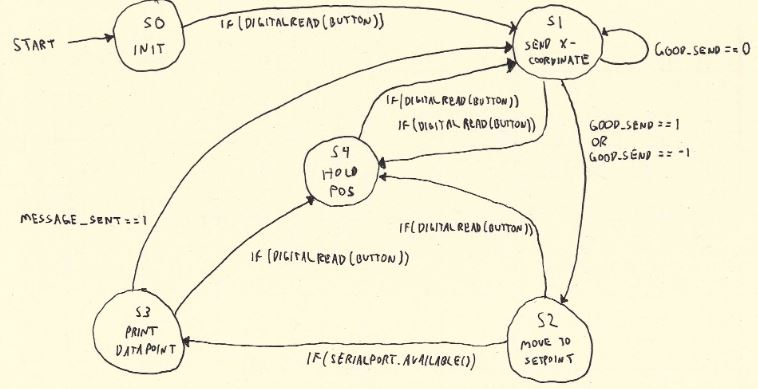
\includegraphics[width=\textwidth]{foshipfsm}
	\caption{Finite-state machine diagram for Fo-SHIP code}
	\label{fig:foshipfsm}
\end{figure}

\noindent In the initialization state, the program does the following:

\begin{itemize}[noitemsep,topsep=0pt]
	\item Initializes the GPIO pins for each MPU6050 and for the input button
	\item Begins the serial connection with the STM32 and the laptop
	\item Initializes the MPU6050s, setting their sensitivity and data rates
	\item Makes the top platform pitch forward and backward to show that the system is working
	\item Performs any demonstration functions if they are selected (see Section \ref{ssec:2s5s6})
\end{itemize}

After this, it waits until the button is pressed before entering the main loop. This gives time for the iSBL array to initialize and get an initial orientation estimate.

Once the button is pressed and the main loop begins, the following sequence repeats until the button is pressed again (in which case, it pauses and restarts the loop). This sequence is meant for data collection --- for a fixed transmitter location, the Fo-SHIP will move through a variety of points and record the position estimate from the STM32 and the acoustic positioning system algorithm, then compare it to the true position as estimated by the Fo-SHIP. The loop executes the following steps:

\begin{itemize}[noitemsep,topsep=0pt]
	\item Calculates the axes that it should iterate through (XYZ or ABC)
	\item For each axis to iterate through, it does the following:
	
	\begin{itemize}[noitemsep,topsep=3ex]
		\item Based on the next setpoint of the Fo-SHIP, sends the x-coordinate of the iSBL array's center to the STM32
		\item Moves to the next setpoint for that axis (for example, moves from Z = 5mm to Z = 4mm)
		\item Waits while the acoustic positioning system algorithm calculates a position estimate for the current setpoint
		\item Prints a datapoint to the laptop's serial connection containing multiple position estimates from the acoustic positioning system algorithms, and the true position of the platform as calculated by the Fo-SHIP
		\item Repeats from the top of this list until all setpoints for a given axis have been tested (for example, testing all points between X = 20mm and X = -20mm)
	\end{itemize}
\end{itemize}

First, the Fo-SHIP calculates which axes it is going to test for this loop. In testing, it was found helpful to sometimes only test the linear (XYZ) axes, and sometimes only test the rotational (ABC) axes. For the final testing, all axes were tested and a Boolean variable was assigned so that all axes were tested equally. 

\begin{lstlisting}[language=C++]
bool translational_axes = false;
...
if (translational_axes) 
{
	axes[0] = "X";
	axes[1] = "Y";
	axes[2] = "Z";
}
else 
{
	axes[0] = "A";
	axes[1] = "B";
	axes[2] = "C";
}
\end{lstlisting}

The maximum and minimum values of each axis, as well as the step size increment, are defined in the main loop.

\begin{lstlisting}[language=C++]
if (axes[axis] == "X") {
	start_val = 5;
	end_val = -5;
	step_increment = linear_step_increment;
	...
} else if (axes[axis] == "A") {
	start_val = radians(15);
	end_val = radians(-15);
	step_increment = angular_step_increment;
	...
\end{lstlisting}

Then, each axis is tested individually. First, the new position of the platform is calculated, and true orientation compensation is applied as described in Section \ref{ssec:2s5s2}. The Fo-SHIP calculates what the next X-coordinate of the iSBL array’s center will be after this new move is executed. While it would be more accurate to move first, get the new orientation, and use that as the platform’s true position, this approach is preferred; it is easier to implement, is more reliable (don’t have to wait for the IMU to stabilize for its new setpoint), works better timing-wise, and is accurate enough for testing purposes. 

\begin{lstlisting}[language=C++]
for (float current_val = start_val*(1-stationary); current_val >= end_val; current_val -= step_increment*(1-stationary)) {
	platform_t newPos = {0, 0, 0, 0, 0, 0};
	
	if (axes[axis] == "X") newPos.hx_x = current_val;
	else if (axes[axis] == "Y") newPos.hx_y = current_val;
	else if (axes[axis] == "Z") newPos.hx_z = current_val;
	else if (axes[axis] == "A") newPos.hx_a = current_val;
	else if (axes[axis] == "B") newPos.hx_b = current_val;
	else if (axes[axis] == "C") newPos.hx_c = current_val;
	...
	platform_t modPos = newPos;
	float rollDiff = modPos.hx_a - currentPos.hx_a;
	float pitchDiff = modPos.hx_b - currentPos.hx_b;
	float yawDiff = modPos.hx_c - currentPos.hx_c;
	modPos.hx_a = radians(stm_roll/4) + rollDiff;
	modPos.hx_b = radians(stm_pitch/4) + pitchDiff;
	modPos.hx_c = radians(stm_yaw/4) + yawDiff;
	...
	getEndEffectorCoords(&modPos, &modPos, &modPos, &modPos, false);
	...
	float next_val = true_x / 1000;
\end{lstlisting}

The reason for sending the X-coordinate is covered more in Chapter \ref{chap:3c}, but it is necessary for proving a simulated “depth” measurement for the acoustic positioning system algorithm. In the full underwater application, a pressure sensor would provide a depth measurement, which is essential for the iSBL algorithm to work properly with short baselines. Since pressure sensors would not work for the above-water testing here, the true X-coordinate of the iSBL array is sent to the STM32 and is used for depth measurement simulation.

Next, a custom function \verb|sendRobustFloat()| is used to ensure that the \verb|true_x| value is sent to the STM32. The function uses checksums and start/end characters to ensure robust data transmission. Initially, there were many unexpected issues with sending data to the STM32 from the ESP32 (but not the other way around), which may suggest a faulty TX-to-RX wire. This function is called up to three times; once a message is sent, if the checksum calculated by the STM32 does not match the one sent by the ESP32, the STM32 instructs the ESP32 to send a message again. If this fails three times, the datapoint is skipped.

\begin{lstlisting}[language=C++]
void sendRobustFloat(float value) {
	char message[50];
	int messageLength = snprintf(message, sizeof(message), "%.4f", value);
	
	int checksum = 0;
	for (int i = 0; i < messageLength; i++) {
		checksum += message[i];
	}
	checksum %= CHECKSUM_MODULUS;
	
	SerialPort.print(START_MARKER);
	SerialPort.print(message);
	SerialPort.print(',');
	SerialPort.print(checksum);
	SerialPort.print(END_MARKER);
	SerialPort.println();
	
	// ensure transmission is complete
	SerialPort.flush();
}
\end{lstlisting}

Multiple times in the code, a blocking \verb|while()| loop is used. A block similar to the one below is used to allow the button press to be registered (to reset the data collection or pause it) when a blocking function is necessary.

\begin{lstlisting}[language=C++]
while (!SerialPort.available()){
	
	// if the button is pressed,
	if (digitalRead(BUTTON)){
		
		// turn the LED on
		digitalWrite(LED, HIGH);
		
		// move back to home
		moveSlowly(&currentPos, &home_coords[0], 20, binaryToDecimal(move_str));
		currentPos = {0, 0, 0, 0, 0, 0};
		
		// break out of all the loops
		shouldBreak = true;
		
		// turn the LED back off
		digitalWrite(LED, LOW);
		Serial.println("BUTTON PRESSED, 1");
		
		// wait until the button is pressed again to resume testing
		while (!digitalRead(BUTTON)){}
		digitalWrite(LED, HIGH);
		delay(1000);
		break;
	}
}
\end{lstlisting}

Once the next X-coordinate is sent, the Fo-SHIP executes the move to the next setpoint. Depending on the type of test being run (gradual or rapid movement), the Fo-SHIP moves at a different speed. Every movement uses the custom \verb|moveSlowly()| function, which linearly interpolates between the current setpoint and the desired (next) setpoint. Notably, the function moves each platform to the same setpoint --- it would need to be modified to control each platform individually.

\begin{lstlisting}[language=C++]
void moveSlowly(platform_t *startCoords, platform_t *endCoords, uint16_t num_steps, uint8_t which_platform) {
	platform_t startPos = *startCoords;
	platform_t endPos = *endCoords;
	int8_t movOK = -1;
	
	for (uint16_t step = 0; step < num_steps; step++) {
		double t = ((double)step) / (double)num_steps;
		
		// linearly interpolate between startPos and endPos
		platform_t interpPos;
		interpPos.hx_x = startPos.hx_x + t * (endPos.hx_x - startPos.hx_x);
		interpPos.hx_y = startPos.hx_y + t * (endPos.hx_y - startPos.hx_y);
		interpPos.hx_z = startPos.hx_z + t * (endPos.hx_z - startPos.hx_z);
		interpPos.hx_a = startPos.hx_a + t * (endPos.hx_a - startPos.hx_a);
		interpPos.hx_b = startPos.hx_b + t * (endPos.hx_b - startPos.hx_b);
		interpPos.hx_c = startPos.hx_c + t * (endPos.hx_c - startPos.hx_c);
		
		// calculate servo angles using the interpolated positions
		movOK = 0;
		if (which_platform & (1 << 3)) movOK += hx_servo.calcServoAngles(interpPos, servo_angles0, 0);
		if (which_platform & (1 << 2)) movOK += hx_servo.calcServoAngles(interpPos, servo_angles1, 1);
		if (which_platform & (1 << 1)) movOK += hx_servo.calcServoAngles(interpPos, servo_angles2, 2);
		if (which_platform & (1 << 0)) movOK += hx_servo.calcServoAngles(interpPos, servo_angles3, 3);
		
		hx_servo.updateServos(movOK);
		
		delay(50);
	}
	
	// move to the final position
	movOK = 0;
	if (which_platform & (1 << 3)) movOK += hx_servo.calcServoAngles(endPos, servo_angles0, 0);
	if (which_platform & (1 << 2)) movOK += hx_servo.calcServoAngles(endPos, servo_angles1, 1);
	if (which_platform & (1 << 1)) movOK += hx_servo.calcServoAngles(endPos, servo_angles2, 2);
	if (which_platform & (1 << 0)) movOK += hx_servo.calcServoAngles(endPos, servo_angles3, 3);
	hx_servo.updateServos(movOK);
}
\end{lstlisting}

Once the Fo-SHIP moves to its new position, it waits while the iSBL array records an acoustic pulse and the STM32 calculates new position estimates. Once the STM32 sends its results over, the ESP32 decodes the serial string, parses the information, and prints the important results to the laptop via UART. Notably, the ESP32 also includes the true position of the iSBL array, which the STM32 does not have access to for its calculations (besides the X-coordinate).

\begin{lstlisting}[language=C++]
String readSerialString() {
	String receivedString = "";
	while (SerialPort.available()) {
		char c = SerialPort.read();
		if (c == '\r' || c == '\n') {
			break;
		}
		receivedString += c;
		delay(2);
	}
	receivedString.trim();
	return receivedString;
}
// once the STM32 sends its data, parse it and put the data into floats
String receivedString = readSerialString();
float x_kf, y_kf, z_kf, x_r_isbl, y_r_isbl, z_r_isbl, x_isbl, y_isbl, z_isbl;
sscanf(receivedString.c_str(), "%f,%f,%f,%f,%f,%f,%f,%f,%f,%f,%f,%f", 
&x_kf, &y_kf, &z_kf, &x_r_isbl, &y_r_isbl, &z_r_isbl, 
&x_isbl, &y_isbl, &z_isbl, &stm_roll, &stm_pitch, &stm_yaw);

// once we have the new orientation of the platform, use it to recalculate the true end effector pos
modPos = currentPos;
modPos.hx_a = radians(stm_roll/4);
modPos.hx_b = radians(stm_pitch/4);
modPos.hx_c = radians(stm_yaw/4);
getEndEffectorCoords(&modPos, &modPos, &modPos, &modPos, false);

// since XYZ and ABC have different units, we need to format the current value differently
float printval;
printval = degrees(current_val*4);
if (translational_axes) printval = current_val*4;

// print a single datapoint / row
Serial.println(String(axes[axis]) + ", " + String(printval)+ ": "
+ String(x_kf) + ", " + String(y_kf) + ", " + String(z_kf) + "; " 
+ String(x_r_isbl) + ", " + String(y_r_isbl) + ", " + String(z_r_isbl) +"; "
+ String(x_isbl) + ", " + String(y_isbl) + ", " + String(z_isbl) + "; "
+ String(true_x) + ", " + String(true_y) + ", " + String(true_z) + "; "
+ String(stm_roll) + ", " + String(stm_pitch) + ", " + String(stm_yaw) +";");
\end{lstlisting}

This process repeats until all values in an axis have been tested. Then, the next axis is tested until all three axes for that loop are iterated through. Then, the variable \verb|translational_axes| flips its value, and the other three axes are tested.

There is additional code for transmitting large chunks of data (like the entire \verb|adc_buf| data, as described in Chapter 3), but it is currently commented out.

\subsection{Multi-Platform Forward Kinematics Calculations} \label{ssec:2s5s4}
Similar to the deep reinforcement learning implementation in Section \ref{ssec:2s1s2}, the large-scale forward kinematics model assumes that each platform can be represented by two vectors: a translational vector defining the distance from the center of the base of a platform to the center of the top of a platform, and a rotational vector defining the vector normal to the top of the platform. Additionally, each platform has a constant offset in its local Z-coordinate to account for the height of the servos. Figure \ref{fig:forwardkine} below shows the forward kinematics model in two dimensions, but the math scales to three dimensions.

\begin{figure}[!htbp]
	\centering
	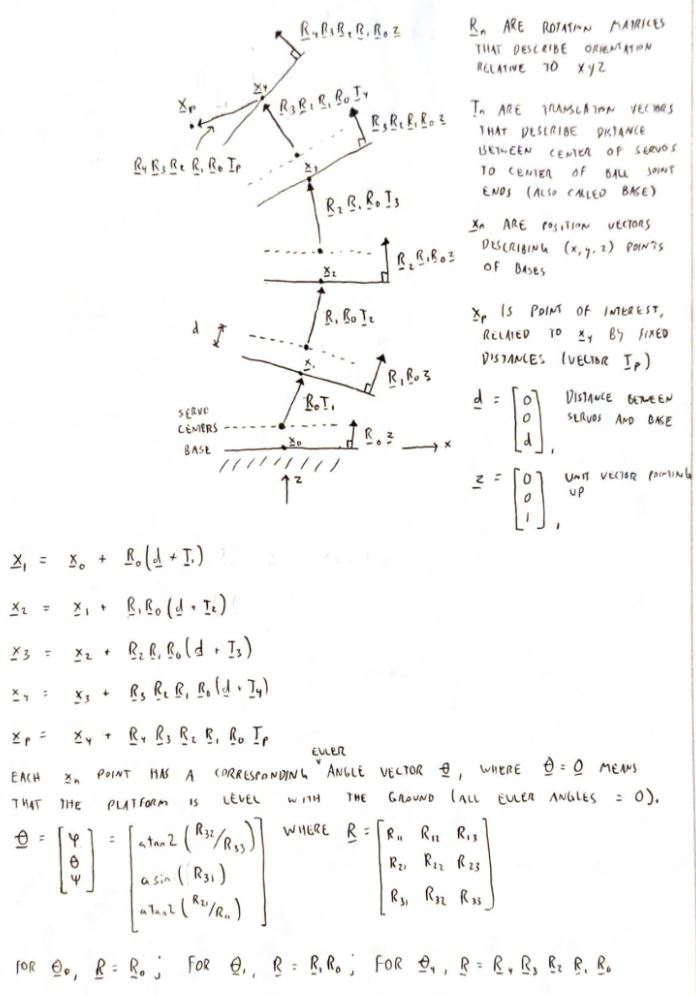
\includegraphics[width=0.9\textwidth]{forwardkine}
	\caption{Forward kinematics diagram}
	\label{fig:forwardkine}
\end{figure}

In the diagram, there are some items to note. First, the Z-axis is pointing in the opposite direction to the final implementation. Next, we work from the base up to the top, applying the previous rotation matrix to each subsequent level. Point xP denotes the center of the iSBL array, which has a constant offset vector which is rigidly attached to the top platform’s end effector. Each rotation matrix (R1, R3, etc.) is defined relative to the platform beneath it, not to the global frame --- the second platform’s base’s rotation in the global frame is described by R2\(\times\)R1\(\times\)R0, but its rotation relative to the platform beneath it is just R2.

This forward kinematics model was implemented in the main code of the Fo-SHIP with the function below. The values \verb|true_x|, \verb|true_y|, and \verb|true_z| are then accessible by the rest of the program when needed.

\begin{lstlisting}[language=C++]
void getEndEffectorCoords(platform_t *coords1, platform_t *coords2, platform_t *coords3, platform_t *coords4, bool USE_IMU){
	float d[3] = {0, 0, -34};
	float TP[3] = {80 + 30, 0, -78.38 - 4};
	float zhome = static_cast<float>(Z_HOME);
	
	float T1[3] = {static_cast<float>(coords1->hx_x), static_cast<float>(coords1->hx_y), static_cast<float>(coords1->hx_z) + zhome};
	float T2[3] = {static_cast<float>(coords2->hx_x), static_cast<float>(coords2->hx_y), static_cast<float>(coords2->hx_z) + zhome};
	float T3[3] = {static_cast<float>(coords3->hx_x), static_cast<float>(coords3->hx_y), static_cast<float>(coords3->hx_z) + zhome};
	float T4[3] = {static_cast<float>(coords4->hx_x), static_cast<float>(coords4->hx_y), static_cast<float>(coords4->hx_z) + zhome};
	
	float eul1[3] = {0, 0, static_cast<float>(coords1->hx_c)};
	float eul2[3] = {0, 0, static_cast<float>(coords2->hx_c)};
	float eul3[3] = {0, 0, static_cast<float>(coords3->hx_c)};
	float eul4[3] = {0, 0, static_cast<float>(coords4->hx_c)};
	
	if (USE_IMU) {
		eul1[0] = IMU1_Angles[0];
		eul1[1] = IMU1_Angles[1];
		eul2[0] = IMU2_Angles[0];
		eul2[1] = IMU2_Angles[1];
		eul3[0] = IMU3_Angles[0];
		eul3[1] = IMU3_Angles[1];
		eul4[0] = IMU4_Angles[0];
		eul4[1] = IMU4_Angles[1];
	} else {
		eul1[0] = static_cast<float>(coords1->hx_a);
		eul1[1] = static_cast<float>(coords1->hx_b);
		eul2[0] = static_cast<float>(coords2->hx_a);
		eul2[1] = static_cast<float>(coords2->hx_b);
		eul3[0] = static_cast<float>(coords3->hx_a);
		eul3[1] = static_cast<float>(coords3->hx_b);
		eul4[0] = static_cast<float>(coords4->hx_a);
		eul4[1] = static_cast<float>(coords4->hx_b);
	}
	
	float R0[9] = {1, 0, 0, 0, 1, 0, 0, 0, 1};
	float R1[9] = {1, 0, 0, 0, 1, 0, 0, 0, 1};
	float R2[9] = {1, 0, 0, 0, 1, 0, 0, 0, 1};
	float R3[9] = {1, 0, 0, 0, 1, 0, 0, 0, 1};
	float R4[9] = {1, 0, 0, 0, 1, 0, 0, 0, 1};
	
	float R1R0[9] = {1, 0, 0, 0, 1, 0, 0, 0, 1};
	float R2R1R0[9] = {1, 0, 0, 0, 1, 0, 0, 0, 1};
	float R3R2R1R0[9] = {1, 0, 0, 0, 1, 0, 0, 0, 1};
	float R4R3R2R1R0[9] = {1, 0, 0, 0, 1, 0, 0, 0, 1};
	
	getRotMatFromEuler(eul1, R1);
	getRotMatFromEuler(eul2, R2);
	getRotMatFromEuler(eul3, R3);
	getRotMatFromEuler(eul4, R4);
	
	multiply3x3Matrices(R1, R0, R1R0);
	multiply3x3Matrices(R2, R1R0, R2R1R0);
	multiply3x3Matrices(R3, R2R1R0, R3R2R1R0);
	multiply3x3Matrices(R4, R3R2R1R0, R4R3R2R1R0);
	
	float x0[3] = {0, 0, -30};
	float dT1[3] = {d[0] + T1[0], d[1] + T1[1], d[2] + T1[2]};
	float x1[3];
	multiply3x3MatrixVector(R0, dT1, x1);
	x1[0] += x0[0];
	x1[1] += x0[1];
	x1[2] += x0[2];
	
	float dT2[3] = {d[0] + T2[0], d[1] + T2[1], d[2] + T2[2]};
	float x2[3];
	multiply3x3MatrixVector(R1R0, dT2, x2);
	x2[0] += x1[0];
	x2[1] += x1[1];
	x2[2] += x1[2];
	
	float dT3[3] = {d[0] + T3[0], d[1] + T3[1], d[2] + T3[2]};
	float x3[3];
	multiply3x3MatrixVector(R2R1R0, dT3, x3);
	x3[0] += x2[0];
	x3[1] += x2[1];
	x3[2] += x2[2];
	
	float dT4[3] = {d[0] + T4[0], d[1] + T4[1], d[2] + T4[2]};
	float x4[3];
	multiply3x3MatrixVector(R3R2R1R0, dT4, x4);
	x4[0] += x3[0];
	x4[1] += x3[1];
	x4[2] += x3[2];
	
	float xP[3];
	multiply3x3MatrixVector(R4R3R2R1R0, TP, xP);
	xP[0] += x4[0];
	xP[1] += x4[1];
	xP[2] += x4[2];
	
	true_x = xP[0];
	true_y = xP[1];
	true_z = xP[2];
}
\end{lstlisting}

Of particular note is the argument \verb|USE_IMU|; if this is set to true, then the Euler angles for each setpoint are replaced by the current angles detected by the MPU6050s. These angles are calculated as described at the end of Section \ref{ssec:2s5s2}.

With the current workaround of using the iSBL array’s IMU to estimate the true orientation of each platform, these estimated angles are inserted into the setpoint coordinates directly, so \verb|USE_IMU| is not currently used.

\subsection{Single-Platform Inverse Kinematics Derivation} \label{ssec:2s5s5}
The inverse kinematics for a single platform describe what angles each servo should be in order to achieve a given \verb|platform_t| setpoint. This implementation uses Algorithm 3 of Jeanmonod’s implementation \cite{nichub} with some modifications, which can be found in \verb|Hexapod_KinematicsCalcServoAnglesAlgo3.h|.

First, a coordinate transform is applied. This thesis assumes an X-forward, Y-left, and Z-down coordinate system, slightly different from the coordinate frame established by Jeanmonod in Figure \ref{fig:hexparams}.

\begin{lstlisting}[language=C++]
double temp = coord.hx_x;
coord.hx_x = -coord.hx_y;
coord.hx_y = -temp;
temp = coord.hx_a;
coord.hx_a = -coord.hx_b;
coord.hx_b = -temp;
coord.hx_c = -coord.hx_c;
coord.hx_z = -coord.hx_z;
\end{lstlisting}

In the algorithm, each servo’s angle is calculated independently from the rest. For the rest of this explanation, a single servo’s calculation is explained. See Figure \ref{fig:hexparams} for important points marked on the platform.

First, the vector \(BP\) is determined. This vector points from the center of the servo horn’s rotation axis to the point where the ball joint must move to. For Stewart platforms, the inverse kinematics tend to be quite easy: to move the platform to a certain position and orientation, apply the transformation to each of the joints on the top of the platform and set the actuator length to the length of \(BP\). For example, to move a platform from X = 0mm to X = 5mm, each point \(P\) is shifted 5mm along the X-axis. The code below shows how \(BP\) is calculated for this implementation.

\begin{lstlisting}[language=C++]
double BP_x = P_COORDS[sid][0] * cosB * cosC + P_COORDS[sid][1] * (sinA * sinB * cosC - cosA * sinC) + coord.hx_x - B_COORDS[sid][0];
double BP_y = P_COORDS[sid][0] * cosB * sinC + P_COORDS[sid][1] * (sinA * sinB * sinC + cosA * cosC) + coord.hx_y - B_COORDS[sid][1];
double BP_z = -P_COORDS[sid][0] * sinB + P_COORDS[sid][1] * sinA * cosB + coord.hx_z - Z_HOME;
\end{lstlisting}

Once BP is determined, it is rotated from the platform coordinate frame into the servo’s local coordinate frame.

\begin{lstlisting}[language=C++]
double
a = COS_THETA_S[sid] * BP_x + SIN_THETA_S[sid] * BP_y,
b = -SIN_THETA_S[sid] * BP_x + COS_THETA_S[sid] * BP_y,
c = BP_z,
...
\end{lstlisting}

In the servo’s local coordinate frame, \(B\) is located at \((0, 0, 0)\), \(A\) (the connection between the rod linkage and the servo horn arm) is located at some point \((x, 0, z)\), and \verb|P| is located at \((a, b, c)\). The rod linkage has length \(R\), and the servo arm has length \(L\). To find the angle that the servo arm should set to, two equations need to be satisfied:

\begin{equation}\label{eq:2eq1}
	(x-a)^2 + b^2 + (z-c)^2 = L^2
\end{equation}

\begin{equation}\label{2eq2}
	x^2 + z^2 = R^2
\end{equation}

These equations describe the relationship between the rod linkage length and the servo arm length. The equations can be combined and expanded to get the following:

\begin{equation}\label{eq:2eq3}
	L^2 + a^2 + b^2 + c^2 - R^2 - 2ax - 2cz = 0
\end{equation}

The servo arm should be set to an angle $\theta$, which forms a right triangle with adjacent side \(x\), opposite side \(z\), hypotenuse \(L\), and nearest angle $\theta$. From this triangle, the relationship can be shown:

\begin{equation}\label{eq:2eq4}
	\tan(\theta) = \frac{z}{x}
\end{equation}

The goal is to form a quadratic equation from Equations \ref{eq:2eq3} and \ref{eq:2eq4}, and this can be achieved by defining:

\begin{equation}\label{eq:2eq5}
	t = \tan( \frac{\theta}{2} ) = \frac{z}{2x}
\end{equation}

Using half-angle identities, it can be shown that:

\begin{equation}\label{eq:2eq6}
	\sin(\theta) = \frac{2t}{1+t^2}
\end{equation}

\begin{equation}\label{eq:2eq7}
	\cos(\theta) = \frac{1-t^2}{1+t^2}
\end{equation}

Using the triangle from before, additional expressions for \(x\) and \(z\) can be formed:

\begin{equation}\label{eq:2eq8}
	x = L\cos(\theta) = L*\frac{1-t^2}{1+t^2}
\end{equation}

\begin{equation}\label{eq:2eq9}
	z = L\sin(\theta) = L*\frac{2t}{1+t^2}
\end{equation}

Substituting into the original equations gives:

\begin{equation}\label{eq:2eq10}
	L^2 + a^2 + b^2 + c^2 - R^2 - 2 \frac{aL(1-t^2) + (cL(2t)}{1+t^2} = 0
\end{equation}

This equation can be fully expanded into the quadratic form below:

\begin{equation}\label{eq:2eq11}
	t^2(L^2 + a^2 + b^2 + c^2 - R^2 + 2aL) + t(-4cL) + (L^2 + a^2 + b^2 + c^2 - R^2 - 2aL) = 0
\end{equation}

\begin{equation}\label{eq:2eq12}
	t^2(A) + t(B) + (C) = 0
\end{equation}

The solution to this equation, assuming the negative square root for stability, is:

\begin{equation}\label{eq:2eq13}
	t = \frac{-B - \sqrt{B^2 - 4AC}}{2A}
\end{equation}

If the term inside the square root, \(B^2 - 4AC\), is negative, then the given setpoint has no valid servo angle to reach it. This term is checked with the lines below, with \verb|i1 = B^2 - 4AC|:

\begin{lstlisting}[language=C++]
double i1 = -ARM_LENGTH4 - ROD_LENGTH4 - a4 - b4 - c4 + 2 * (ARM_LENGTH2 * (ROD_LENGTH2 + a2 - b2 + c2) + ROD_LENGTH2 * (a2 + b2 + c2) - a2 * (b2 + c2) - b2 * c2);
if (i1 < 0)
{
	movOK = -5;
	break;
}
\end{lstlisting}

Assuming that the term is positive and valid, the next step is to take the square root of \verb|i1| and solve the quadratic:

\begin{lstlisting}[language=C++]
double rt_i1 = sqrt(i1);
double i2 = (2 * ARM_LENGTH * c - rt_i1) /
(ARM_LENGTH2 + 2 * ARM_LENGTH * a -
ROD_LENGTH2 + BP2);
\end{lstlisting}

Lastly, the term \verb|i2 = t|, and the original expression for \verb|t| is solved for $\theta$:

\begin{lstlisting}[language=C++]
double i3 = 2 * atan(i2);
\end{lstlisting}

The double \verb|i3| now contains the angle for this singular servo in radians, which is converted to a PWM signal and set in the \verb|Hexapod_Servo| class. This process is repeated for each servo.

\subsection{Demonstration Functions} \label{ssec:2s5s6}
The last functions for the Fo-SHIP are related to some demonstration modes. These functions include:

\begin{itemize}[noitemsep,topsep=0pt]
	\item Reaching the minimum and maximum positions for each axis
	\item Moving in a circle about the pitch and roll axes (largest possible movements for the Fo-SHIP)
	\item Actively tracking the transmitter by moving the pitch and yaw axes to point the iSBL array directly towards it
\end{itemize}

The first is quite simple --- it works almost identically to the main testing code, except it reaches the full range-of-motion for each axis. First, it moves each platform the same; each platform moves to its maximum X-value, then minimum X-value, then maximum Y-value, and so on. After the last axis (C) has been actuated, it then moves the second and third platform in an inverted manner. So, for the X-axis, the first and fourth platforms move to the maximum X-value while the second and third move to the minimum X-value. This motion forces the end effector to stay fully stationary for the translational axes and level for the rotational axes.

The circle demonstration shows the speed and agility of the Fo-SHIP. First, it plots the setpoints to move through for a given radius, starting at the maximum value of the roll axis and rotating between the roll and pitch axes.

\begin{lstlisting}[language=C++]
for (uint8_t angleID = 0; angleID < nb_points; angleID++)
{
	coords[angleID] = {0, 0, 0, (radius * cos(angle)), (radius * sin(angle)), 0};
	angle += angleInc;
}
\end{lstlisting}

The active tracking is more complex and requires some functions from the main loop to communicate with the STM32 and acoustic positioning algorithm. Once a datapoint is collected, the STM32 sends the estimated position of the receiver array as well as the “true” position of the transmitter. For this demonstration, the transmitter is being held and moved, so it does not match the “true” position, but this doesn’t matter --- the vector pointing from the receiver array to the transmitter can be reconstructed from the data sent by the STM32, as shown below. 

\begin{lstlisting}[language=C++]
String receivedString = readSerialString();
float x_kf, y_kf, z_kf, x_r_isbl, y_r_isbl, z_r_isbl, x_isbl, y_isbl, z_isbl, stm_roll, stm_pitch, stm_yaw, x_tx, y_tx, z_tx;
sscanf(receivedString.c_str(),"%f,%f,%f,%f,%f,%f,%f,%f,%f,%f,%f,%f,%f,%f,%f", 
&x_kf, &y_kf, &z_kf, &x_r_isbl, &y_r_isbl, &z_r_isbl, 
&x_isbl, &y_isbl, &z_isbl, &stm_roll, &stm_pitch, &stm_yaw,
&x_tx, y_tx, z_tx);

// calculate the angle to move the Fo-SHIP to point the iSBL array at the transmitter
float pitch, yaw;
float x_latx = x_tx - x_isbl;
float y_latx = y_tx - y_isbl;
float z_latx = z_tx - z_isbl;
pitch = atan2f(z_latx, x_latx);
yaw = atan2f(y_latx, x_latx);
new_pos.hx_b += pitch/4;
new_pos.hx_c += yaw/4;
moveSlowly(&current_pos, &new_pos, 14, binaryToDecimal(1111));
current_pos = new_pos;
\end{lstlisting}

After determining the vector point from the receiver array to the transmitter, the Fo-SHIP determines the pitch and yaw movement required to point directly at the transmitter. The movement is then executed.

\section{System Calibration} \label{sec:2s6}
Careful calibration of the servo offsets is required to produce accurate positioning for the Fo-SHIP. A go/no-go gauge was manufactured to ensure that each servo horn was level with the rest when at a neutral position.

\begin{figure}[htbp]
	\centering
	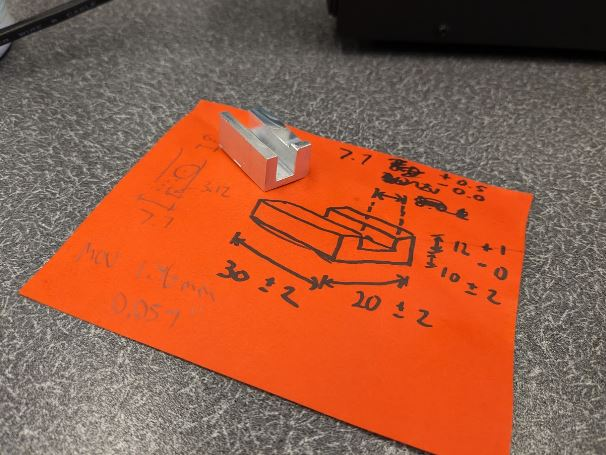
\includegraphics[width=0.8\textwidth]{gaugedrawing}
	\caption{Go/no-go gauge drawing and part}
	\label{fig:gaugedrawing}
\end{figure}

\begin{figure}[htbp]
	\centering
	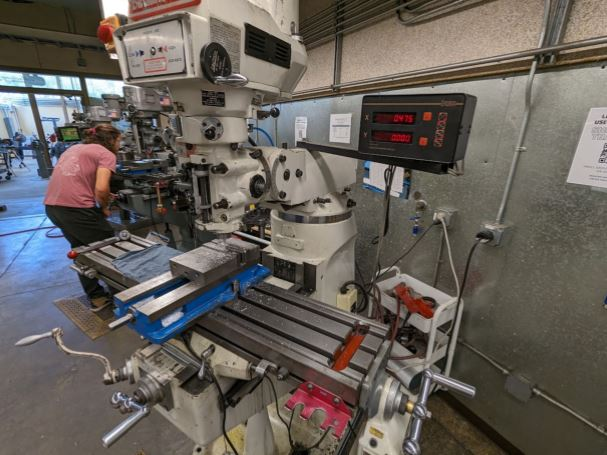
\includegraphics[width=0.8\textwidth]{mill}
	\caption{Manufacturing of go/no-go gauge on mill in Mustang ‘60 Machine Shop}
	\label{fig:mill}
\end{figure}

\noindent Each pair of servos was leveled according to the following workflow:

\begin{itemize}[noitemsep,topsep=0pt]
	\item Set all platforms to a setpoint (0, 0, 10, 0, 0, 0) where all servos should be level, power the Fo-SHIP, and move the platforms to the setpoint
	\item Test each pair of servos with the gauge by attempting to fit the width of both servo horn arms between the channel of the gauge
	\item If little-to-no force is required to fit the servo horn arms between the gauge’s channel, then that pair of servos is level
	\item If a moderate amount of force is required to fit the arms or if they are unable to fit in the gauge, then the servo offsets in \verb|PW_OFFSET[]| in \verb|Hexapod_Config1.h| need to be adjusted
	\item Adjust the servo offsets by a small amount in the direction of the misalignment; if both servo arms have a downward slope from the base to the tip of the servo horn, then add an offset that will make the servos turn upright
	\item Repeat this process, applying the new offset values and testing each pair of servos, until all servo horns are level
\end{itemize}

Each servo horn is between 7.5mm and 7.8mm in width and between 24.5mm and 25.5mm in length between connection holes. The go-no-go gauge has a width of 7.85mm and a length of 31.4mm. The spacing between servos is between 57mm and 59mm. In a worst-case scenario, both servo horns are 7.5mm wide and 24.5mm long, and the spacing between servos is 59mm. The relationship between these constants and the maximum angular misalignment between the servos is derived below.

\begin{figure}[htbp]
	\centering
	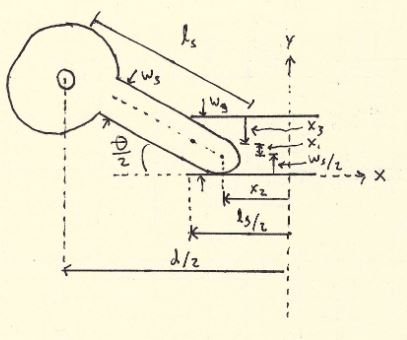
\includegraphics[width=0.9\textwidth]{misalign}
	\caption{Servo misalignment diagram (exaggerated scale)}
	\label{fig:misalign}
\end{figure}

The goal is to find an equation that relates the angle $\theta$ to the constants of the physical setup. By comparing the vertical components of the servo horn arm with the width of the gauge, we can find the following equations:

\begin{equation}\label{eq:2eq14}
	x_2 = \frac{d}{2} - l_s cos(\frac{\theta}{2})
\end{equation}

\begin{equation}\label{eq:2ew15}
	x_1 = (\frac{l_g}{2} - x_2) \times \frac{sin(\frac{\theta}{2})}{cos(\frac{\theta}{2})}
\end{equation}

\begin{equation}\label{eq:2eq16}
	x_3 = \frac{w_s}{2cos(\frac{\theta}{2})}
\end{equation}

\begin{equation}\label{eq:2eq17}
	w_g = \frac{w_s}{2} + x_1 + x_3
\end{equation}

This system of equations was solved using the constants from above using Python to get a maximum angular error of 3.7° between servos when using the go/no-go gauge. This angular misalignment is a worst-case scenario and not all servos are misaligned to this degree, but it’s important to take into consideration when considering sources of error.

\begin{lstlisting}[language=C++]
import numpy as np
from scipy.optimize import fsolve

# Givens
ws = 7.5
ls = 24.5
wg = 7.85
lg = 31.4
d = 59

# Calculate
def equations(vars):
	theta = vars
	x2 = d/2 - ls * np.cos(theta/2)
	x1 = (lg/2 - x2) * np.sin(theta/2) / np.cos(theta/2)
	x3 = ws / (2 * np.cos(theta/2))
	eq1 = ws/2 + x1 + x3 - wg
	return eq1

theta_ans = fsolve(equations, (0))  # Initial guess
print(np.degrees(theta_ans))
\end{lstlisting}

\section{System Testing and Validation} \label{sec:2s7}
Once the servos were calibrated and all of the code was functioning, it was imperative to verify the accuracy of the Fo-SHIP’s position estimate. A variety of positions were tested and measured multiple times, and the averages of these measurements were recorded. Table \ref{tab:foshipvalid} summarizes the positions tested, the estimated XYZ position of the iSBL array’s center, and the measured XYZ position of the iSBL array’s center. The measured values have an uncertainty of ±1.6mm due to the measurement devices used. All units are in millimeters, and the absolute error is computed as the L2 distance from the estimated point to the measured point. The estimated XYZ position is calculated using the forward kinematics model described in Section \ref{ssec:2s5s4} and uses the IMU on the iSBL array for orientation estimation.

\begin{table}[htbp]
	\centering
	\caption{Fo-SHIP position validation}
	\label{tab:foshipvalid}
	\renewcommand{\arraystretch}{1.2}
	\begin{tabular}{|c|c|c|c|c|c|c|c|}
		\hline
		Position & Est. X & Est. Y & Est. Z & Meas. X & Meas. Y & Meas. Z & Abs. Err. \\
		\hline
		Zero & 124 & 1 & -642 & 127 & 0 & -643 & 3.32 \\
		\hline
		Max X & 152 & 1 & -638 & 152 & 2 & -639 & 1.41 \\
		\hline
		Max Y & 126 & 21 & -642 & 127 & 19 & -643 & 2.45 \\
		\hline
		Min Z & 122 & -2 & -708 & 126 & -1 & -711 & 5.10 \\
		\hline
		Max Roll & 90 & 305 & -520 & 101 & 295 & -535 & 21.12 \\
		\hline
		Min Pitch & 333 & 4 & -425 & 340 & 2 & -430 & 8.83 \\
		\hline
		Med Roll & 111 & 178 & -604 & 105 & 172 & -610 & 10.39 \\
		\hline
		Med Pitch & 263 & 2 & -542 & 257 & 1 & -543 & 6.16 \\
		\hline
	\end{tabular}
\end{table}

The average positional error of the Fo-SHIP when using the IMU orientation compensation is 7.35mm. The maximum error measured was 21.12mm (for the maximum possible displacement), and the positional error tends to grow as the pitch and roll increase.

\noindent This error comes from a variety of sources:

\begin{itemize}[noitemsep,topsep=0pt]
	\item Angular misalignment for the servo horns, as described in the previous section
	\item Slop in the system from servos not holding their precise angle due to loading
	\item Potentially loose connections from the heat-set inserts moving during testing
	\item Slight bending on some of the threaded rod linkages from repeated testing
	\item Inaccurate measurement of parameters for a single platform as defined in the code
	\item Measurement inaccuracy from above testing
\end{itemize}

While this error is larger than desired, it is acceptable given the low-cost nature of the actuator. Better actuators and metal base plates would significantly improve the positioning accuracy of the Fo-SHIP. For any future implementations, it is recommended to use linear actuators in place of rotational servos and to use machined metal plates with smaller tolerances than the 3D printed components used here.





%-------------------------CHAPTER 3-------------------------





\chapter{Acoustic Positioning System} \label{chap:3c}
The acoustic positioning system is the core of the iSBL-SF algorithm. In this system, an acoustic pulse is sent by a transmitter and recorded by receivers on the iSBL array. The time shift between the signals from each receiver is calculated, and these shifts are used to estimate the transmitter’s position relative to the iSBL array using an acoustic propagation model. Chapter \ref{chap:4c} describes how the orientation estimate of the platform is determined (and how dead reckoning is introduced), and Chapter \ref{chap:5c} details how Kalman filters are used to get the best position estimate by combining multiple data sources. This chapter describes only the acoustic positioning system, the central component of this thesis.

The first section in this chapter is dedicated to previous implementations of acoustic positioning systems, and how the iSBL approach differs from them. Next, the mechanical design of the receiver array is discussed. The electrical design of the acoustic positioning system, including the wiring diagram of the full iSBL array, is then detailed. The ultrasonic receivers receive their own section, where the design and manufacturing of the active band-pass filter PCB is explained. Then, the assembly of the full iSBL array is described, followed by the hardware and software design of the transmitter system. The final three sections are devoted to the software of the acoustic positioning system: how an acoustic pulse is detected and recorded, how the time shift between signals is calculated, and finally, how a position estimate is formed.

\section{Previous Works} \label{sec:3s1}
Acoustic positioning systems are not a new invention, and many different designs have been tested and implemented over the years. The rise of autonomous underwater vehicles has accelerated research into this field. In this section, the history of acoustic positioning systems is recounted, and the primary difference among these systems (the baseline length) is described. Lastly, similar implementations to this thesis are detailed.

\subsection{History of Acoustic Positioning Systems} \label{ssec:3s1s1}
The first known underwater acoustic positioning system was deployed in 1963, when a short baseline acoustic positioning system was used to guide the bathyscape \emph{Trieste 1} to the wreck of the US nuclear submarine USS \emph{Thresher}. The system barely worked, only guiding the \textit{Trieste} to the wreck once after ten unsuccessful attempts. The technology advanced as commercial applications became evident; oil and gas exploration in the 1970s was a primary driver for advancement. In 1998, a long baseline acoustic positioning system was used by a salvage company to navigate a debris field of a sunken WW2 Japanese submarine at 5240m deep. Current advancements in the field are primarily driven by the oil and gas industry, academic research, and defense industry applications \cite{apomab}.

\begin{figure}[htbp]
	\centering
	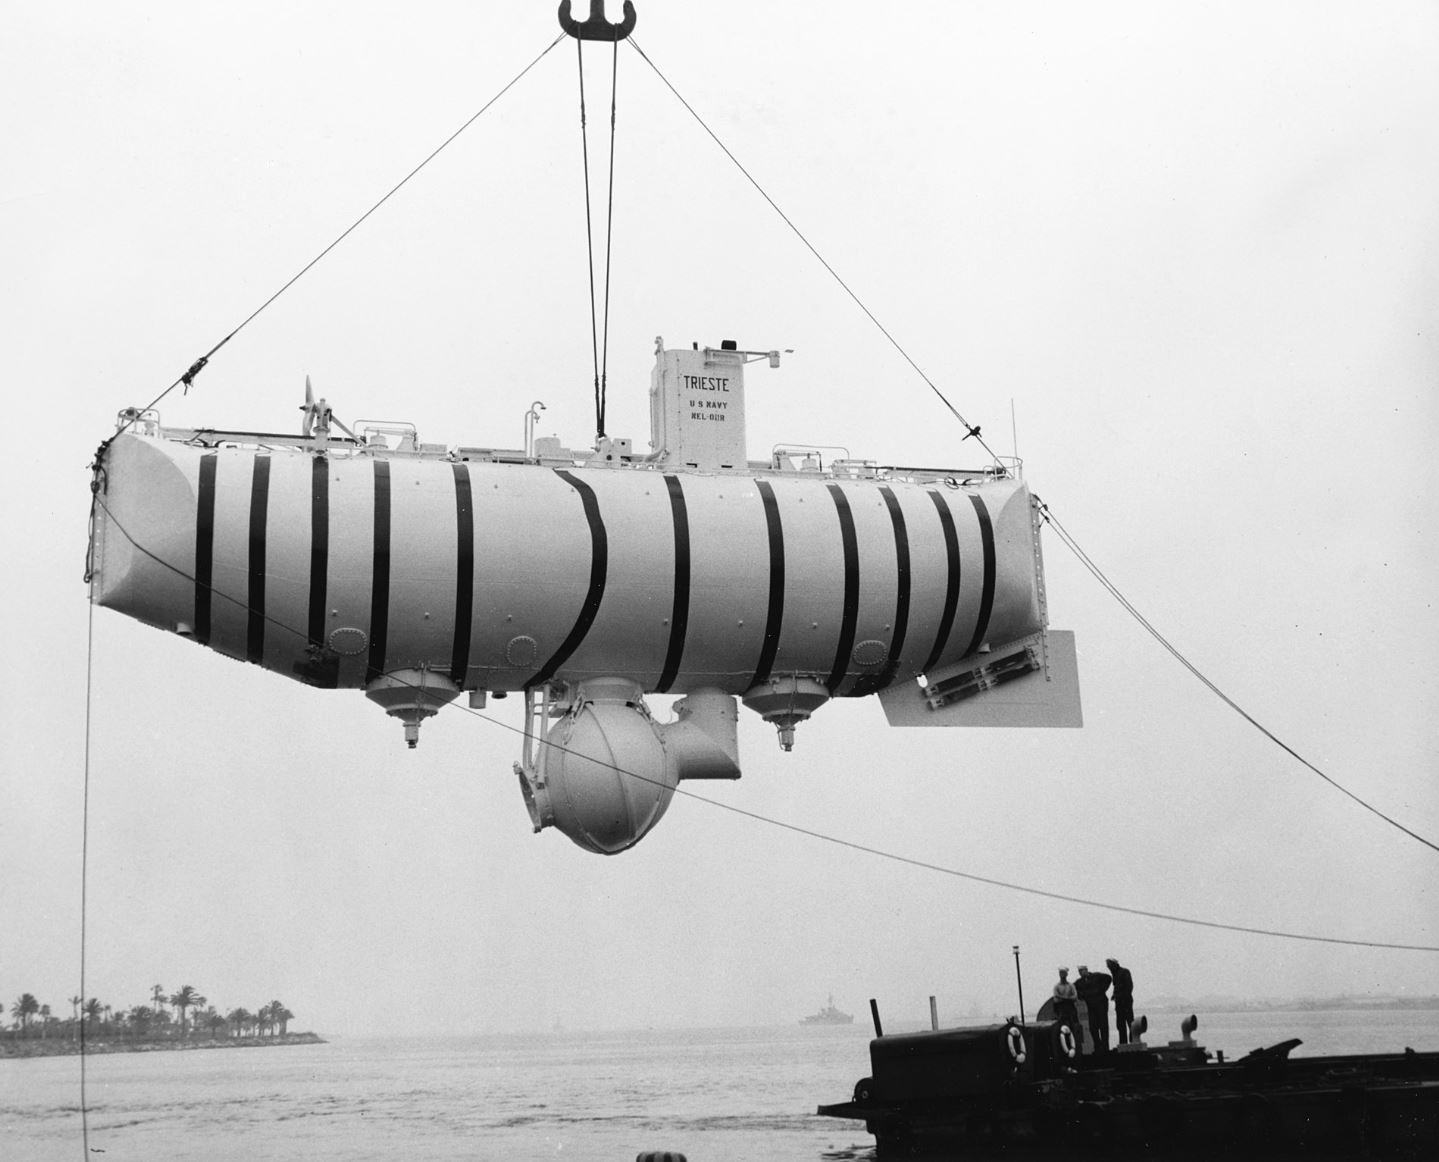
\includegraphics[width=0.5\textwidth]{trieste}
	\caption{Bathyscape \textit{Trieste 1}, which used the first short baseline acoustic positioning system to locate a nuclear submarine wreck \cite{apomab}}
	\label{fig:trieste}
\end{figure}

\subsection{Long, Short, Ultrashort, and Inverted Baselines} \label{ssec:3s1s2}
All acoustic positioning systems use the same core principle to function: sound waves propagate through a medium in a known and predictable way, and by sending acoustic waves from one or more transmitters to one or more receivers, the relative location between the transmitters and receivers can be determined. The primary way of differentiating underwater acoustic positioning systems is by their baseline, the spacing between receivers (or transmitters, depending on the system).

Long baseline (LBL) systems generally use multiple receivers spaced further than 100m apart in known, fixed locations; a transmitter is attached to the moving object whose position estimate is desired. LBL systems tend to have the best position accuracy when properly calibrated, but require many more resources and much more time to set up \cite{practicaloverview}. These systems are preferable when working in a single location for long periods of time and when sub-meter accuracy is desired \cite{apomab}. An additional benefit to LBL systems is that they tend to not require additional measurement equipment such as inertial measurement units or depth sensors, though additional equipment can improve accuracy. See Figure \ref{fig:lbldiagram} for an example of an LBL system.

\begin{figure}[htbp]
	\centering
	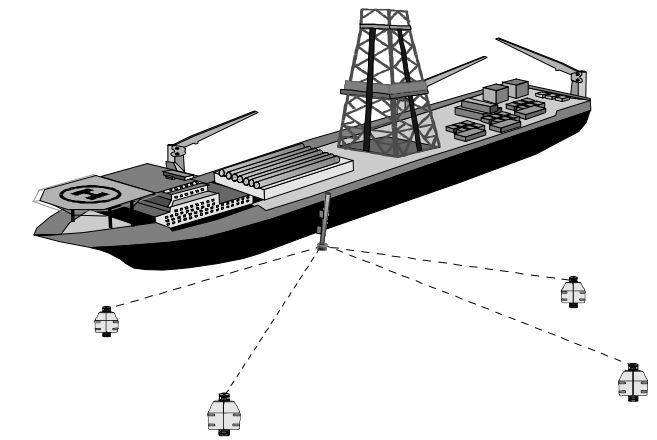
\includegraphics[width=0.5\textwidth]{lbldiagram}
	\caption{Long baseline acoustic positioning system diagram \cite{practicaloverview}}
	\label{fig:lbldiagram}
\end{figure}

Ultrashort baseline (USBL) systems generally use a single receiver module with multiple receiver elements spaced less than 10cm apart. These systems usually apply phase-differencing methods to compute the heading between the transmitter and receiver, with the receiver elements spaced less than one wavelength apart \cite{apomab}. These systems also tend to have low overall complexity and are contained in a single module; however, positional accuracy is less than LBL systems, and additional sensors (orientation sensors, vertical reference units) are required to obtain a position estimate \cite{practicaloverview}. See Figure \ref{fig:usbldiagram} for an example of a USBL system.

\begin{figure}[htbp]
	\centering
	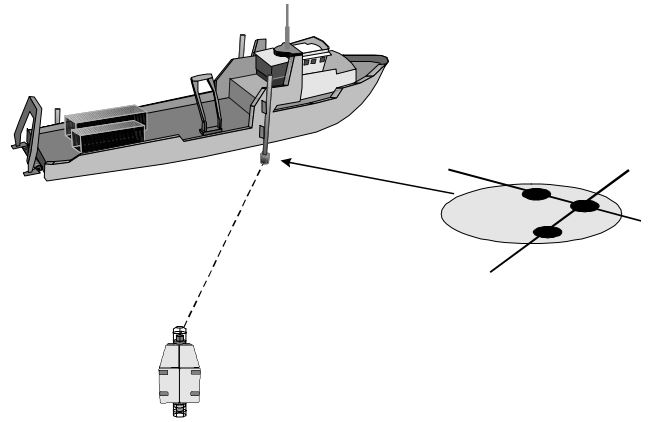
\includegraphics[width=0.5\textwidth]{usbldiagram}
	\caption{Ultrashort baseline acoustic positioning system diagram \cite{practicaloverview}}
	\label{fig:usbldiagram}
\end{figure}

Short baseline (SBL) systems are more broad and tend to encompass acoustic positioning systems whose baseline is greater than one wavelength (typically 1m - 100m) and whose receivers (or transmitters) are not fixed to the seafloor \cite{surveyurpn}. For example, the system of an ROV in the water equipped with a single transmitter and a boat on the surface of the water with receivers on each corner of the hull would be considered an SBL system. SBL systems tend to be a good middle-ground between LBL and USBL: they don’t require a fixed receiver array with massive baselines, but can produce position estimates that approach LBL-level accuracy. These systems do require additional sensors as USBL systems do (orientation and depth), but the receiver array is generally attached to a vessel that already has these systems integrated. See Figure \ref{fig:sbldiagram} for an example of an SBL system.

\begin{figure}[htbp]
	\centering
	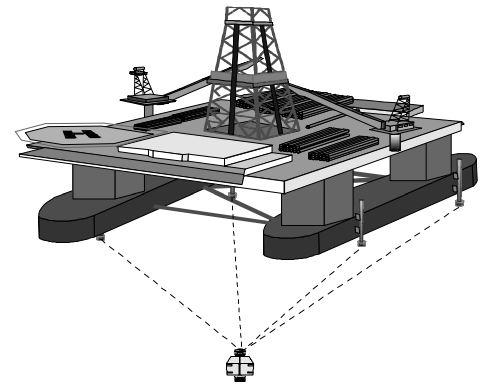
\includegraphics[width=0.5\textwidth]{sbldiagram}
	\caption{Short baseline acoustic positioning system diagram \cite{practicaloverview}}
	\label{fig:sbldiagram}
\end{figure}

Inverted acoustic positioning systems flip the location of the transmitter and receiver arrays. An inverted ultrashort baseline (iUSBL) places the transmitter on the surface of the water (generally on a research vessel or buoy with a known location) and the receiver module on an underwater vehicle --- see Figure \ref{fig:iusblukf} for an example. Due to the small size of USBL system (with the receiver being similar in size to the transmitter), iUSBL systems are quite common, especially in autonomous underwater vehicles \cite{noveliusbl} \cite{passiveiusbl}.

\begin{figure}[htbp]
	\centering
	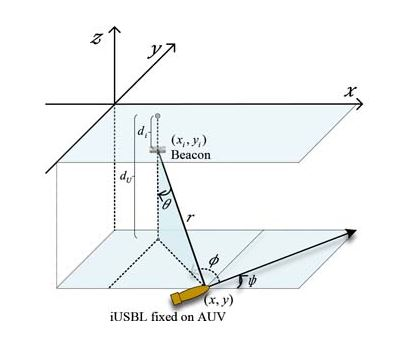
\includegraphics[width=0.6\textwidth]{iusblukf}
	\caption{Inverted ultrashort baseline system example \cite{iusblukf}}
	\label{fig:iusblukf}
\end{figure}

Inverted LBL and SBL systems are much more rare; only one paper espouses an iLBL system, whose diagram is shown in Figure \ref{fig:ilbl} below. Throughout the research for this thesis, no known papers have been written about iSBL systems --- most systems that would use a receiver array on an underwater vehicle tend to space the receivers less than a baseline apart, or otherwise call themselves iUSBL systems.

\begin{figure}[htbp]
	\centering
	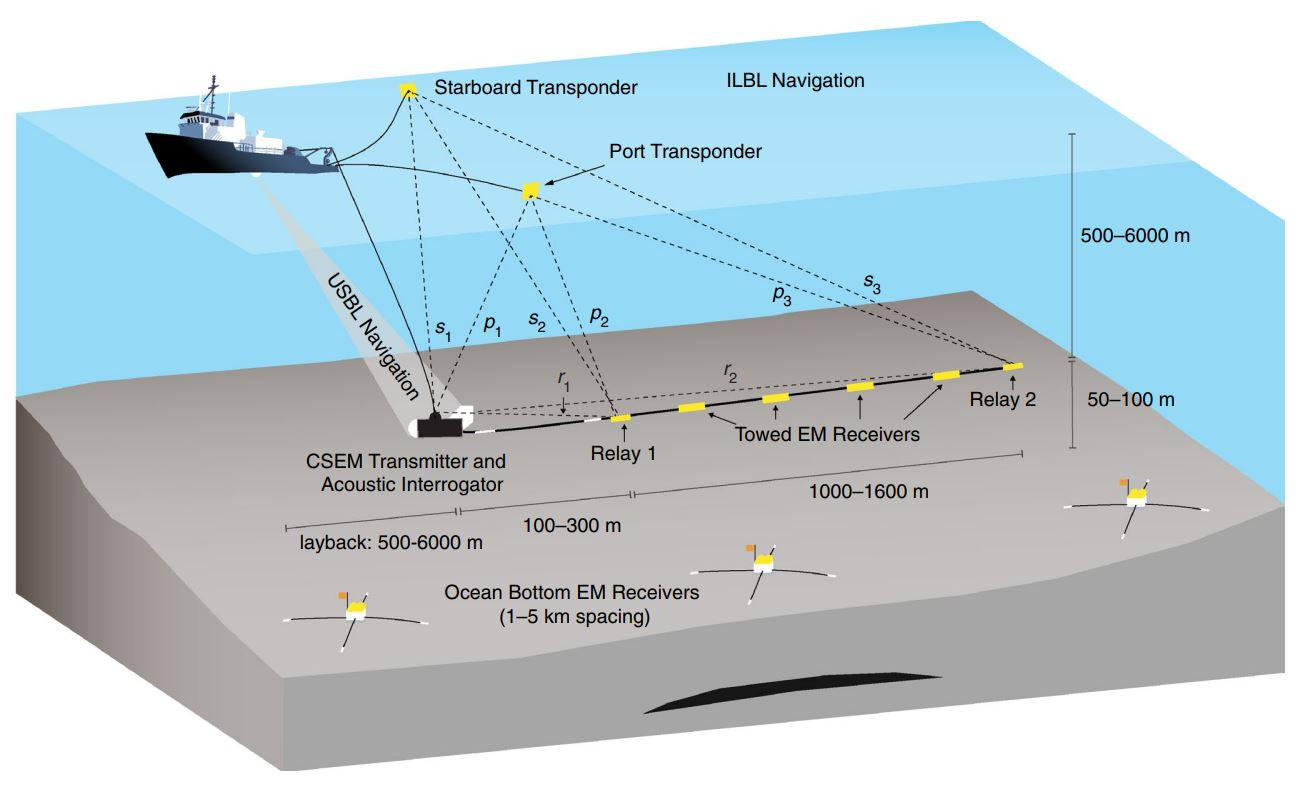
\includegraphics[width=0.65\textwidth]{ilbl}
	\caption{Inverted long baseline system example \cite{ilbl}}
	\label{fig:ilbl}
\end{figure}

In this thesis, an iSBL acoustic positioning system is proposed. While iUSBL systems primarily use phase-differencing and a baseline of less than one wavelength, this proposed iSBL system will use time-differencing and a baseline of greater than one wavelength. The system also uses a single transmitter on the surface of the water (attached to a floating buoy or other autonomous vehicle) and an array of multiple receivers on the underwater vehicle. For a full underwater implementation of this iSBL system, it is recommended to place the receivers as far apart as possible on the body of the underwater vehicle as possible to increase the accuracy of the position estimate.

\subsection{Similar Implementations} \label{ssec:3s1s3}
While the classification of this system as an iSBL system is novel, the design of the system draws upon previous research. Since iUSBL and iSBL are quite similar, some iUSBL systems were studied and used as inspiration for this thesis. Luo and Ko of Hoseo University in South Korea designed an iUSBL system with a floating beacon on the surface of the water, and implemented more complex systems (such as simultaneous mapping and localization algorithms) into their design \cite{iusblukf}. Researchers from Zhejiang University in China implemented an iUSBL system on an autonomous underwater vehicle that uses FPGAs and beamforming to improve the position estimate \cite{passiveiusbl}.

The four most relevant implementations are as follows. Alcocer, Oliveira, and Pascoal from the Institute for Systems and Robotics of Portugal described an acoustic positioning system using GPS Intelligent Buoys (GIBs), which act like a floating LBL system with acoustic and GPS receivers on each buoy \cite{gibs}. Smith and Kronen of the Florida Atlantic University’s Department of Ocean Engineering detailed a low-cost SBL positioning system using a foldable acoustic array \cite{lowcostsbl}. More researchers from Zhejiang University in China created and tested a single-transmitter, variable-baseline acoustic positioning system, the most similar implementation to the one developed in this thesis \cite{singletrans}. Lastly, Morgado, Oliveira, and Silvestre from the Technical University of Lisbon, Portugal tested a USBL system with tightly-coupled inertial measurement devices, which combines the USBL position estimates with an inertial navigation system using an extended Kalman filter \cite{tightekf}.

Finally, a GitHub repository by the Underwater Communication and Navigation Laboratory provided many fantastic examples of acoustic positioning implementations. The UCNLNav repository was instrumental in this implementation, giving a great example of implementing Hooke-Jeeves search for time-difference-of-arrival systems \cite{ucnlnav}. This repository will be revisited later in Section \ref{ssec:3s9s2}.

\section{Receiver Array Mechanical Design} \label{sec:3s2}
The receiver array for this implementation is made of four ultrasonic transducers spaced in an \(\times\)-pattern, with each transducer having a baseline of 25cm from the center. See Figure \ref{fig:isblnaked} for an image of the array without any wiring attached. The array is mounted at a 90° angle relative to the Fo-SHIP’s end effector, pointing towards the X-axis of the Fo-SHIP.

\begin{figure}[htbp]
	\centering
	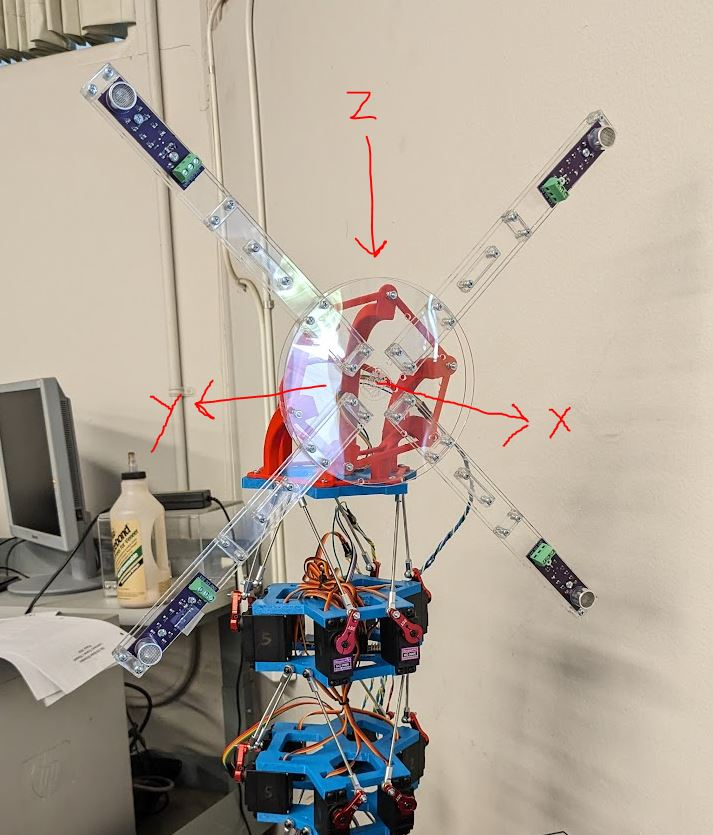
\includegraphics[width=0.5\textwidth]{isblnaked}
	\caption{iSBL array without wiring or microcontroller, with local coordinate system overlaid; X-forward, Y-right, Z-down relative to the face of the array}
	\label{fig:isblnaked}
\end{figure}

The array is constructed from laser-cut 2.4mm-thick acrylic sheet. The components were designed using Solidworks and were cut on the Mustang ‘60 Machine Shop PLS laser cutters. Four long beams are attached to a central circular hub; the microcontroller, soldered breadboard, and IMU have mounting holes on the central hub, while the receivers have mounting holes on the ends of the long beams. The holes are spaced such that the center of the ultrasonic receiver elements are 25cm from the center of the array. A partial CAD model of the array can be seen in Figure \ref{fig:partarray}.

\begin{figure}[htbp]
	\centering
	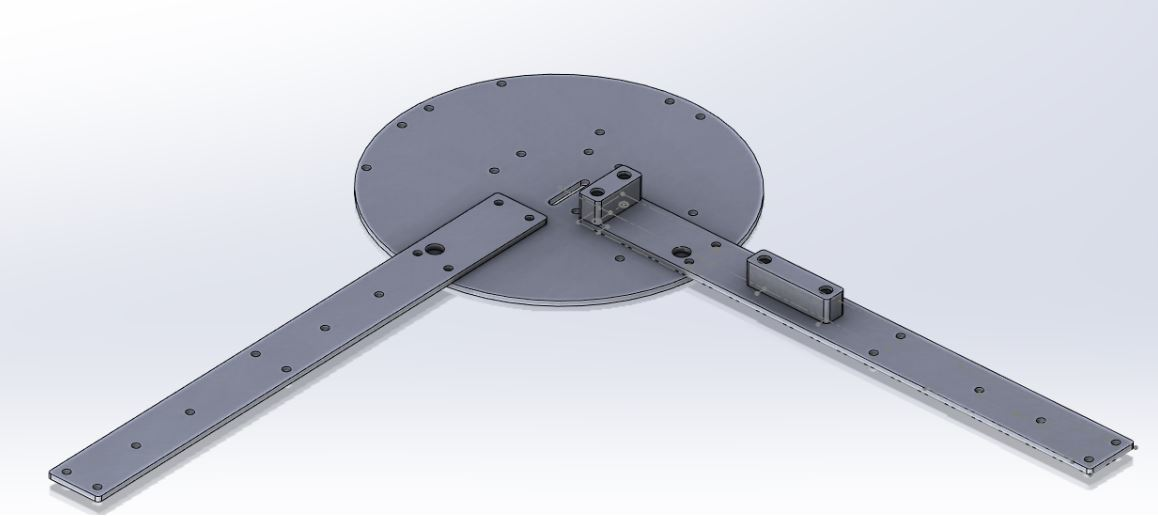
\includegraphics[width=0.7\textwidth]{partarray}
	\caption{Partial CAD model of iSBL array, made using Solidworks}
	\label{fig:partarray}
\end{figure}

Note that the array was constructed from multiple layers of planar acrylic components to reduce the weight of the iSBL array, which affects the overall loading on the Fo-SHIP end effector. The array uses spacer elements to allow for flexibility of the long members, which can help account for any warping of the long, thin elements. Additionally, acrylic sheeting was a low-cost, low-weight, and easy-to-manufacture component when compared to other materials like wood or aluminum. A side view of the array can be seen in Figure \ref{fig:sidearray}.

\begin{figure}[htbp]
	\centering
	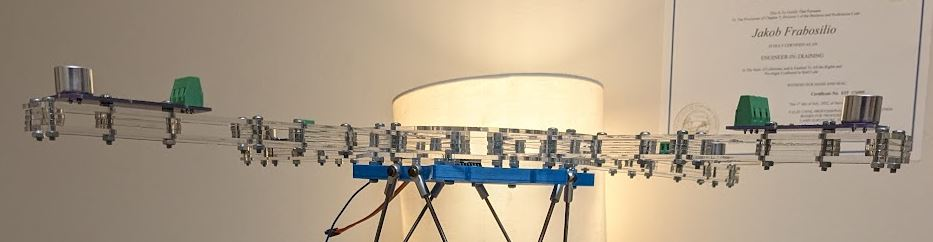
\includegraphics[width=\textwidth]{sidearray}
	\caption{Side view of iSBL array}
	\label{fig:sidearray}
\end{figure}

Lastly, a 90° adapter was printed on a Prusa Mk.3 FDM 3D printer in the Mustang ‘60 Machine Shop. This component is crucial for testing the iSBL-SF algorithm in a horizontal test environment. If the adapter was not added, then the Fo-SHIP would need to be mounted horizontally on a wall (poor loading condition due to gravity), or the transmitter element would need to be suspended in the air above the Fo-SHIP. The adapter was designed in Solidworks and incorporates many lightweighting and stiffening elements. A render of the adapter in 3D printing slicing software can be seen in Figure \ref{fig:sliceradapter}.

\begin{figure}[htbp]
	\centering
	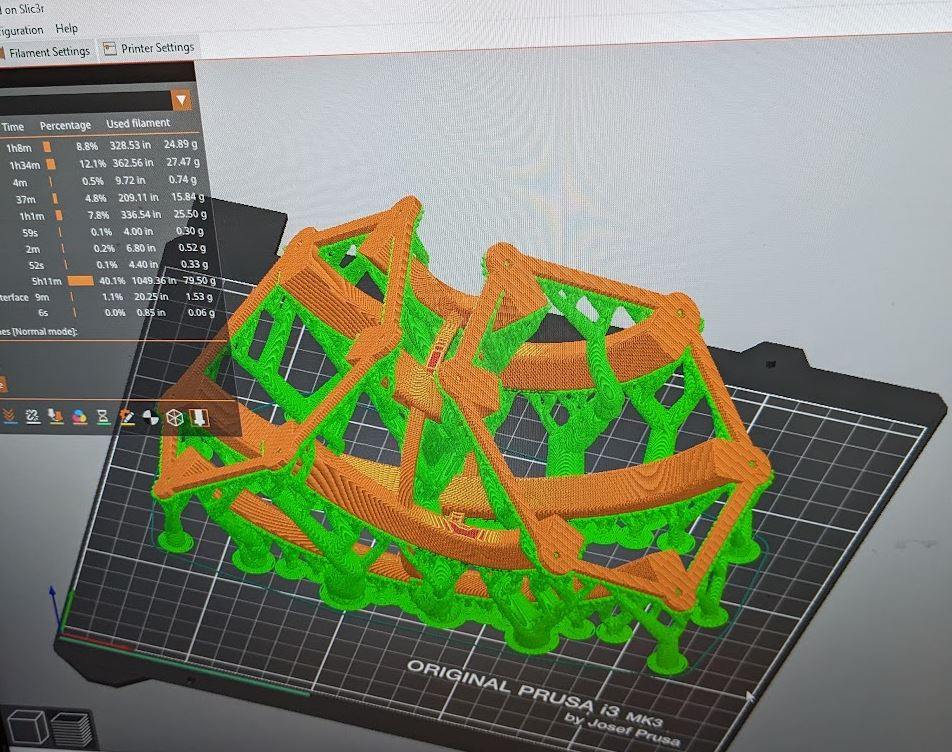
\includegraphics[width=0.6\textwidth]{sliceradapter}
	\caption{iSBL adapter in 3D slicing software (PrusaSlicer)}
	\label{fig:sliceradapter}
\end{figure}

\section{Receiver Array Electrical Design} \label{3s3}
The acoustic positioning system and iSBL array include three main components: the STM32 microcontroller, the receiver elements, and the IMU. The receiver element design is discussed in Section \ref{sec:3s4}, and the IMU selection is discussed in Chapter \ref{chap:4c}. For the rest of this chapter, it will be referred to as “the IMU,” but its full designation is a combined LSM6DSOX 3-axis accelerometer and gyroscope and LIS3MDL 3-axis magnetometer.

The microcontroller used for this project is the STM32H723ZG from STMicroelectronics. This microcontroller was chosen with specific requirements: an analog-to-digital converter (ADC) capable of recording more than 1 million samples per second at 12-bit resolution, random access memory storage greater than 200kB, digital signal processing libraries, and a high-speed CPU clock. The H723ZG fulfills all these requirements \cite{stmdatasheet}, comes on a development board for easy prototyping and implementation, and is very low-cost at around \$30 for one development board \cite{stm144}. The development board is much larger than required for this system with over 114 GPIO pins and 30 ADC channels, so for future implementations, switching to a custom printed circuit board (PCB) would be recommended. An image of the STM32H723ZG development board can be seen in Figure \ref{fig:stm144}.

\begin{figure}[htbp]
	\centering
	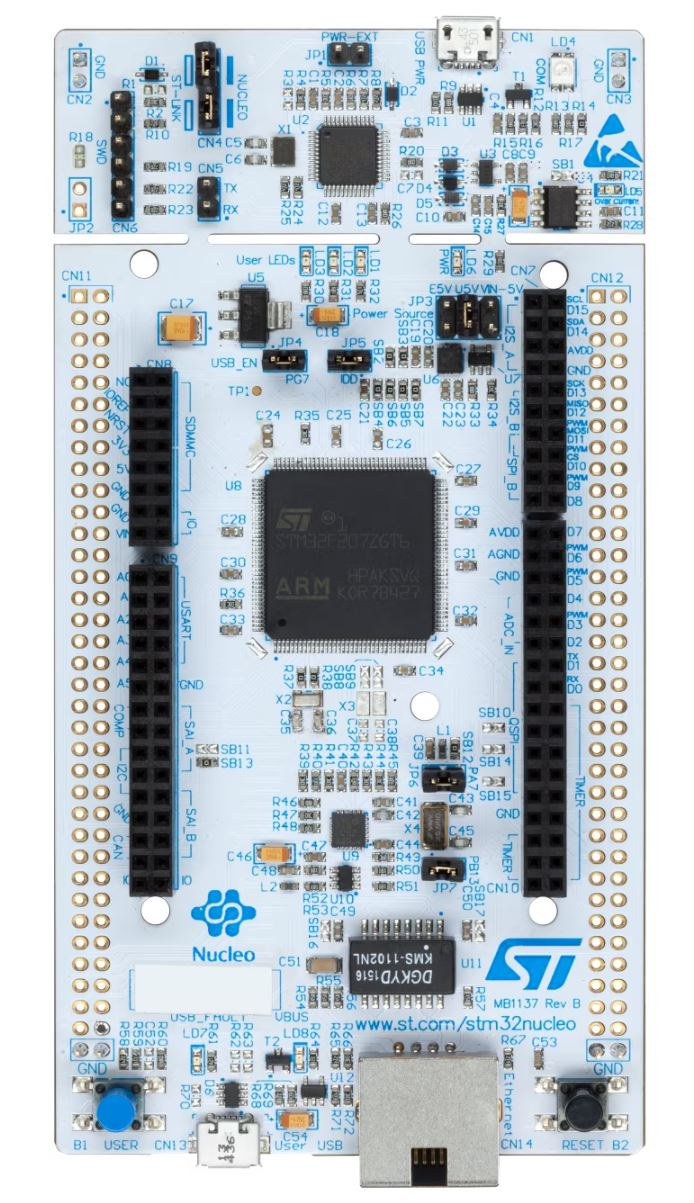
\includegraphics[width=0.25\textwidth]{stm144}
	\caption{STM32H723ZG development board \cite{stm144}}
	\label{fig:stm144}
\end{figure}

For this implementation, four ADC inputs, two GPIO pins, one USB connection, one I\textsuperscript{2}C connection, and one serial connection are used. A wiring diagram in Figure \ref{fig:stmwiring} shows the full schematic of the system. The STM32 communicates with the IMU over I\textsuperscript{2}C, communicates with a laptop via USB, and communicates with the ESP32 controlling the Fo-SHIP via a serial connection. The wiring and communications protocol for I\textsuperscript{2}C and serial are described in Section \ref{sec:2s3}. Each receiver element is connected to an ADC input, as well as a power and ground connection. Four LEDs are used for debugging and testing; three are internal LEDs on the STM32 development board, while one is connected to an external GPIO pin. A second GPIO pin is used as an interrupt for the IMU; when the IMU has new data ready, the STM32 can detect it via this GPIO pin.

\begin{figure}[!htbp]
	\centering
	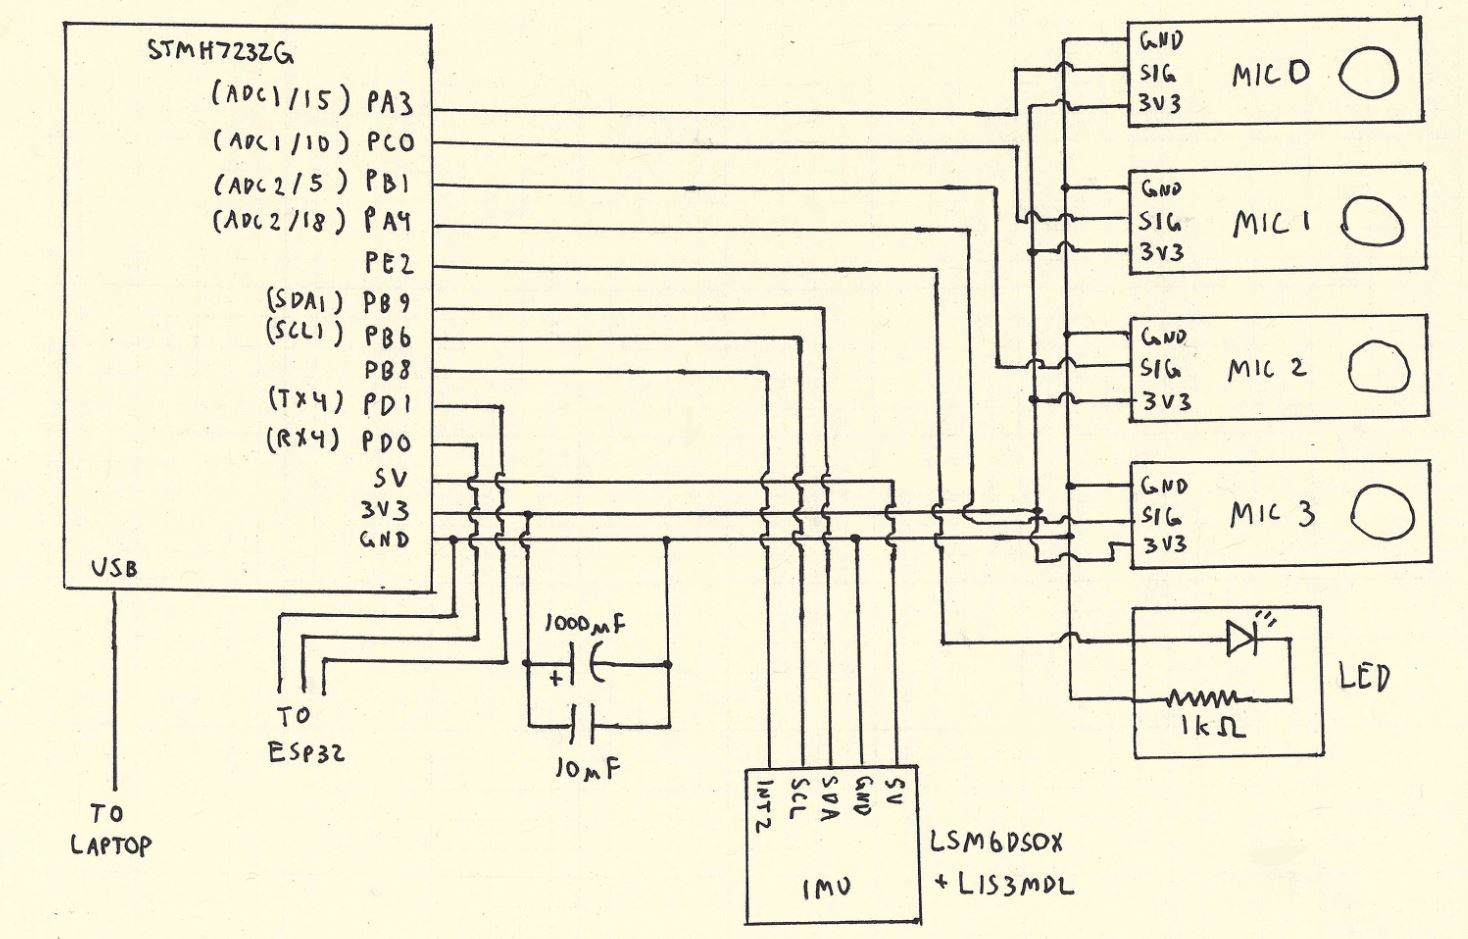
\includegraphics[width=\textwidth]{stmwiring}
	\caption{iSBL system wiring diagram}
	\label{fig:stmwiring}
\end{figure}

Lastly, two capacitors, one large 1000uF electrolytic capacitor and one small 10uF ceramic capacitor, were added to filter out electrical noise from the STM32’s 3v3 line. 

\section{Active Band-Pass Filter Design} \label{sec:3s4}
This implementation is designed to work with 40kHz audio signals. This frequency was chosen for a few reasons:
\begin{itemize}[noitemsep,topsep=0pt,]
	\item The above-water frequency should be similar to the planned underwater system’s frequency to allow for simple future implementation
	\item The audible range should be avoided to minimize disturbance to marine animals (see Section \ref{sec:6s3} for more details on the underwater system extrapolation)
	\item Lower frequencies require lower ADC sampling rates to record a single wave
	\item Lower audio frequencies are attenuated much less rapidly in seawater compared to higher frequencies (see Figure \ref{fig:attenuation})
	\item 40kHz is a very common frequency for air-based ultrasonic transducers, and fairly common in water-based ultrasonic transducers
\end{itemize}

\begin{figure}[htbp]
	\centering
	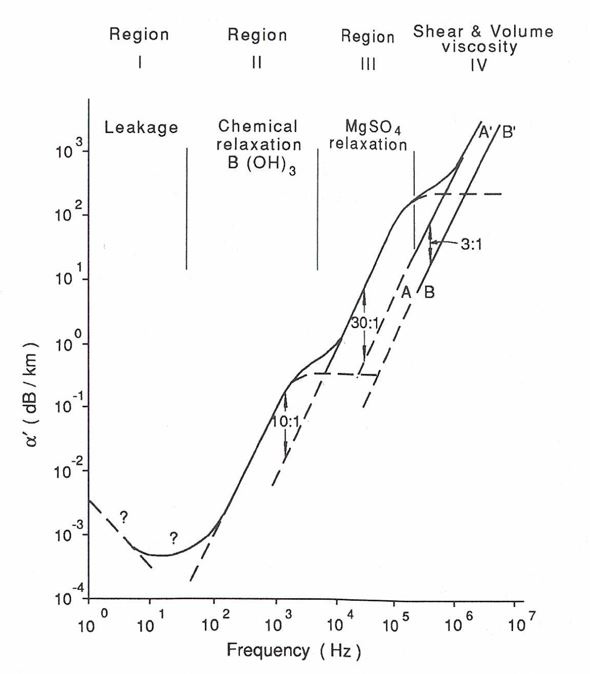
\includegraphics[width=0.65\textwidth]{attenuation}
	\caption{Sound attenuation in seawater with dominant attenuation process regions \cite{computational}}
	\label{fig:attenuation}
\end{figure}

Using ultrasonic transducers without any filtering or amplification would severely limit the range and accuracy of the acoustic positioning system. To overcome both of these issues, an electrical circuit is necessary to:
\begin{itemize}[noitemsep,topsep=0pt,]
	\item Amplify the output voltage of the receiver elements to a sufficient level for the microcontroller’s ADCs
	\item Reject frequencies that are outside of the desired passband
	\item Be inexpensive and scalable to all microphones
	\item Reduce the amount of digital pre-processing required
\end{itemize}

An active band-pass filter is a good solution to the problem and it fulfills the above requirements. Inverting active band-pass filters in particular are designed to have narrow pass-bands. An inverting active band-pass filter based on a circuit from ElectronicsTutorials \cite{abpfws} (see Figure \ref{fig:abpfws}) was used with the following modifications:
\begin{itemize}[noitemsep,topsep=0pt,]
	\item A decoupling capacitor and voltage divider (C3, R3, R4) that adds a 1.65V DC bias to the microphone signal
	\item A voltage divider (R5, R6) that sets the non-inverting input of the op-amp to 1.65V
\end{itemize}

\begin{figure}[htbp]
	\centering
	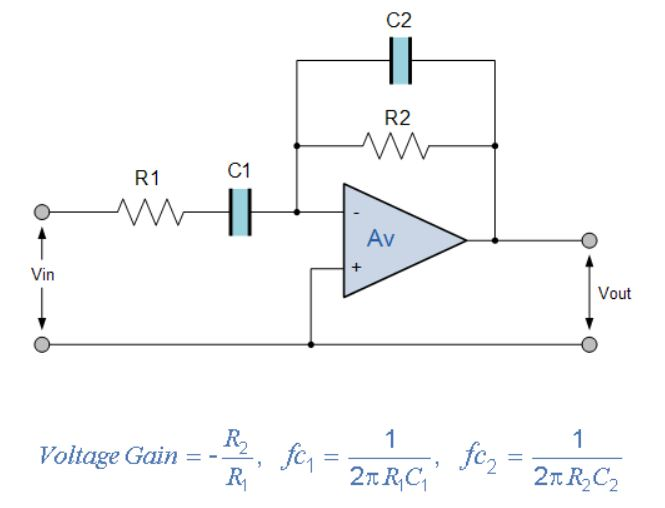
\includegraphics[width=0.8\textwidth]{abpfws}
	\caption{Inverting active band-pass filter \cite{abpfws}}
	\label{fig:abpfws}
\end{figure}

These modifications are necessary for the system to function --- see the modified circuit diagram in Figure \ref{fig:abpfcircuit}. When testing an ultrasonic receiver and transmitter at a distance of 3 meters apart, the receiver registered a peak-to-peak voltage of approximately 10mV when the transmitter was powered by a 12Vpp, 40kHz sine wave. This voltage oscillates around 0V. The ADC on the STM32 is capable of reading voltages between 0V and 3.3V; to maximize the range of the receiver output, a 1.65V DC bias needs to be added to the receiver signal. Since the op-amp is being powered by an asymmetric 0V to 3.3V supply, the inputs must be biased to the center of the supply voltage range to minimize clipping at the rail voltages. This setup ensures that the whole range of the op-amp is used.

The resistor and capacitor values need to be carefully selected to provide proper filtering and amplification; the equations in Figure \ref{fig:abpfws} are the governing equations for this filter. First, a voltage gain of approximately 100 was desired to amplify the 10mVpp signal to 1Vpp; this resulted in a resistor ratio of 100:1. Next, cutoff frequencies close to 38kHz and 42kHz were desired to reduce the amplification of frequencies outside of this passband. After many iterations of resistor and capacitor values (using common values from the E6 and E12 series to avoid using special components and to reduce cost \cite{e6e12}), the values in Figure \ref{fig:abpfcircuit} were chosen. These values result in a gain of -100 and cutoff frequencies of 38.1kHz and 41.3kHz. 

\begin{figure}[!htbp]
	\centering
	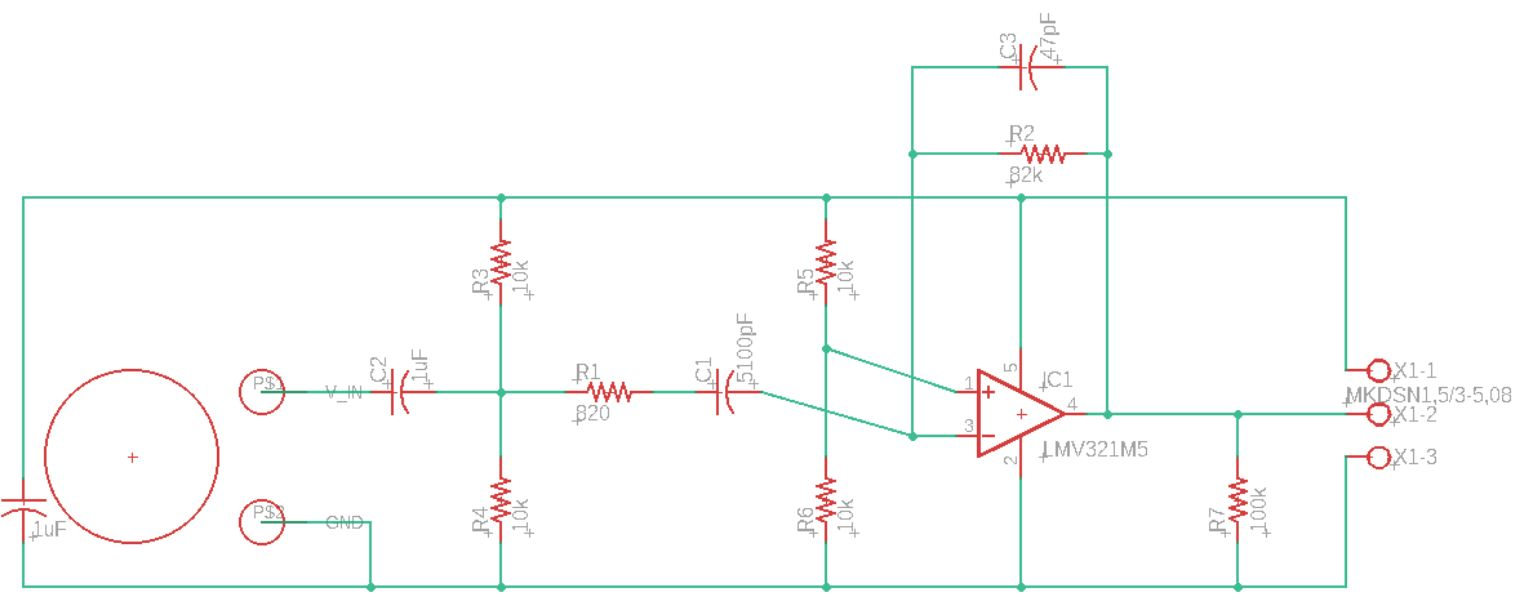
\includegraphics[width=\textwidth]{abpfcircuit}
	\caption{Custom active band-pass filter circuit diagram}
	\label{fig:abpfcircuit}
\end{figure}

The circuit was simulated in LTSpice\textsuperscript{\textregistered}\xspace, an electrical design and simulation software, to validate the design. A sine sweep test with an AC source placed at the ultrasonic transducer element was run; the results can be seen in Figure \ref{fig:ltspice}. The simulation shows a peak amplitude response of 34.5dB at 39kHz, an approximate gain of 53. The filter does not have as sharp of a peak as desired, but the sensitivity curve of the ultrasonic receivers used has a similar curve; these two curves add together to produce a frequency response with a large peak at the resonant frequency of the receiver. See Figure \ref{fig:usrsens} for the sensitivity curve of the receiver.

\begin{figure}[htbp]
	\centering
	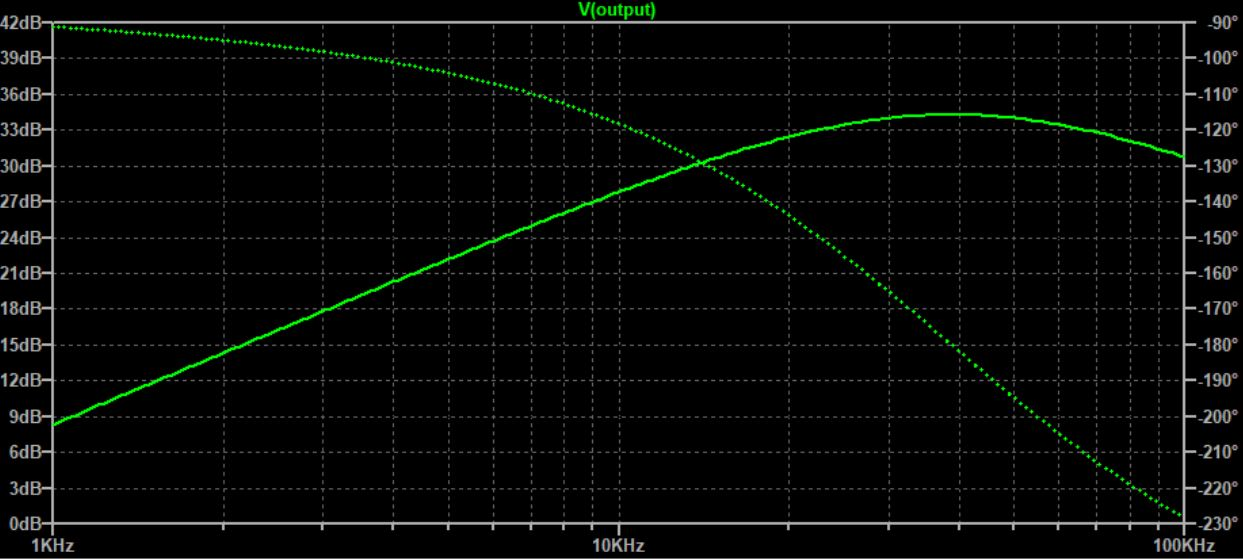
\includegraphics[width=\textwidth]{ltspice}
	\caption{Sine-sweep test of active band-pass filter circuit, run in LTSpice. Solid line is amplitude ratio, dashed line is phase shift}
	\label{fig:ltspice}
\end{figure}

\begin{figure}[htbp]
	\centering
	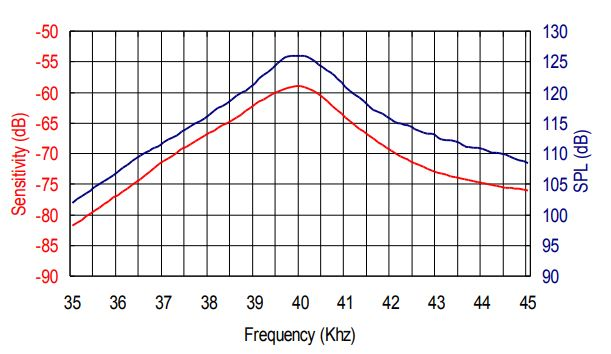
\includegraphics[width=0.6\textwidth]{usrsens}
	\caption{Sensitivity of 400SR160 ultrasonic receiver \cite{400sr160}}
	\label{fig:usrsens}
\end{figure}

After selecting electrical components, the PCB files were designed in Eagle\textsuperscript{\textregistered}\xspace (see Figure \ref{fig:abpfeagleREAL}) and the PCB was then fabricated by OSH Park (a PCB manufacturer based in Oregon). See Figure \ref{fig:abpfeagle} for the rendering of the PCB from OSH Park. The electrical components for the circuit were purchased from Mouser Electronics.

\begin{figure}[htbp]
	\centering
	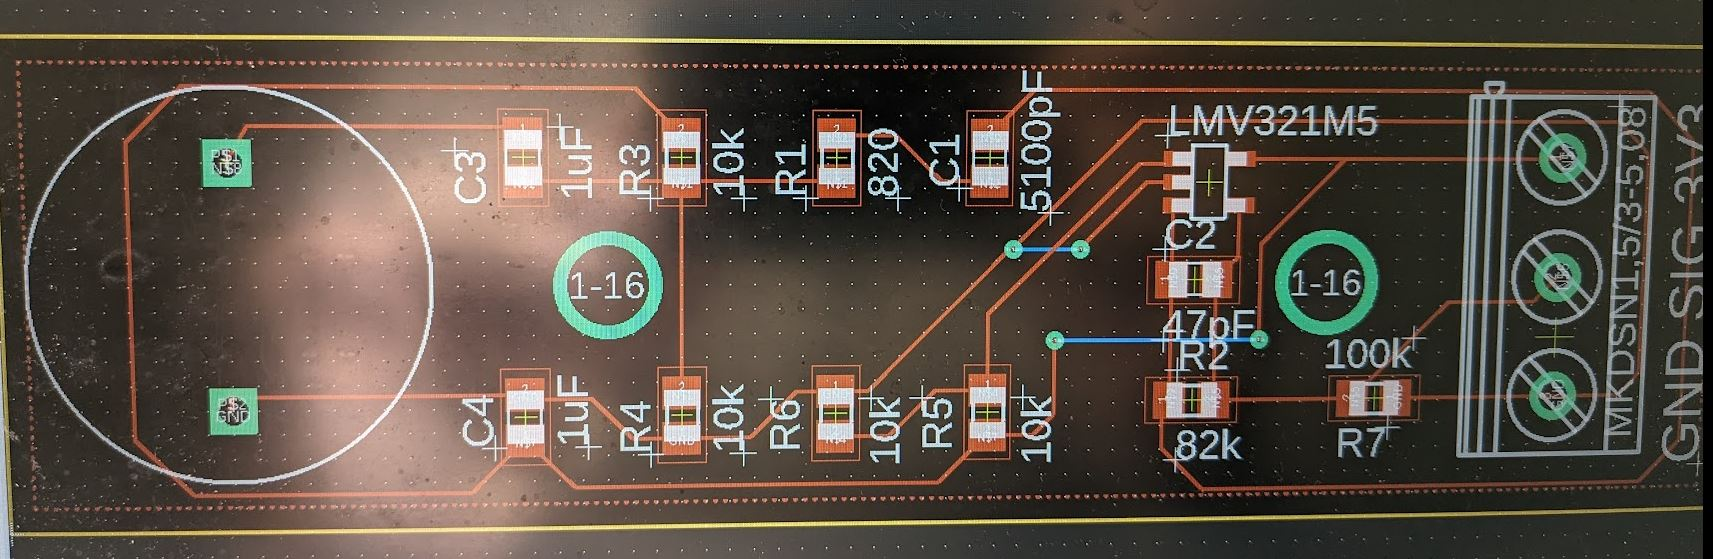
\includegraphics[width=0.7\textwidth]{abpfeagleREAL}
	\caption{Custom active band-pass filter in Eagle}
	\label{fig:abpfeagleREAL}
\end{figure}

\begin{figure}[htbp]
	\centering
	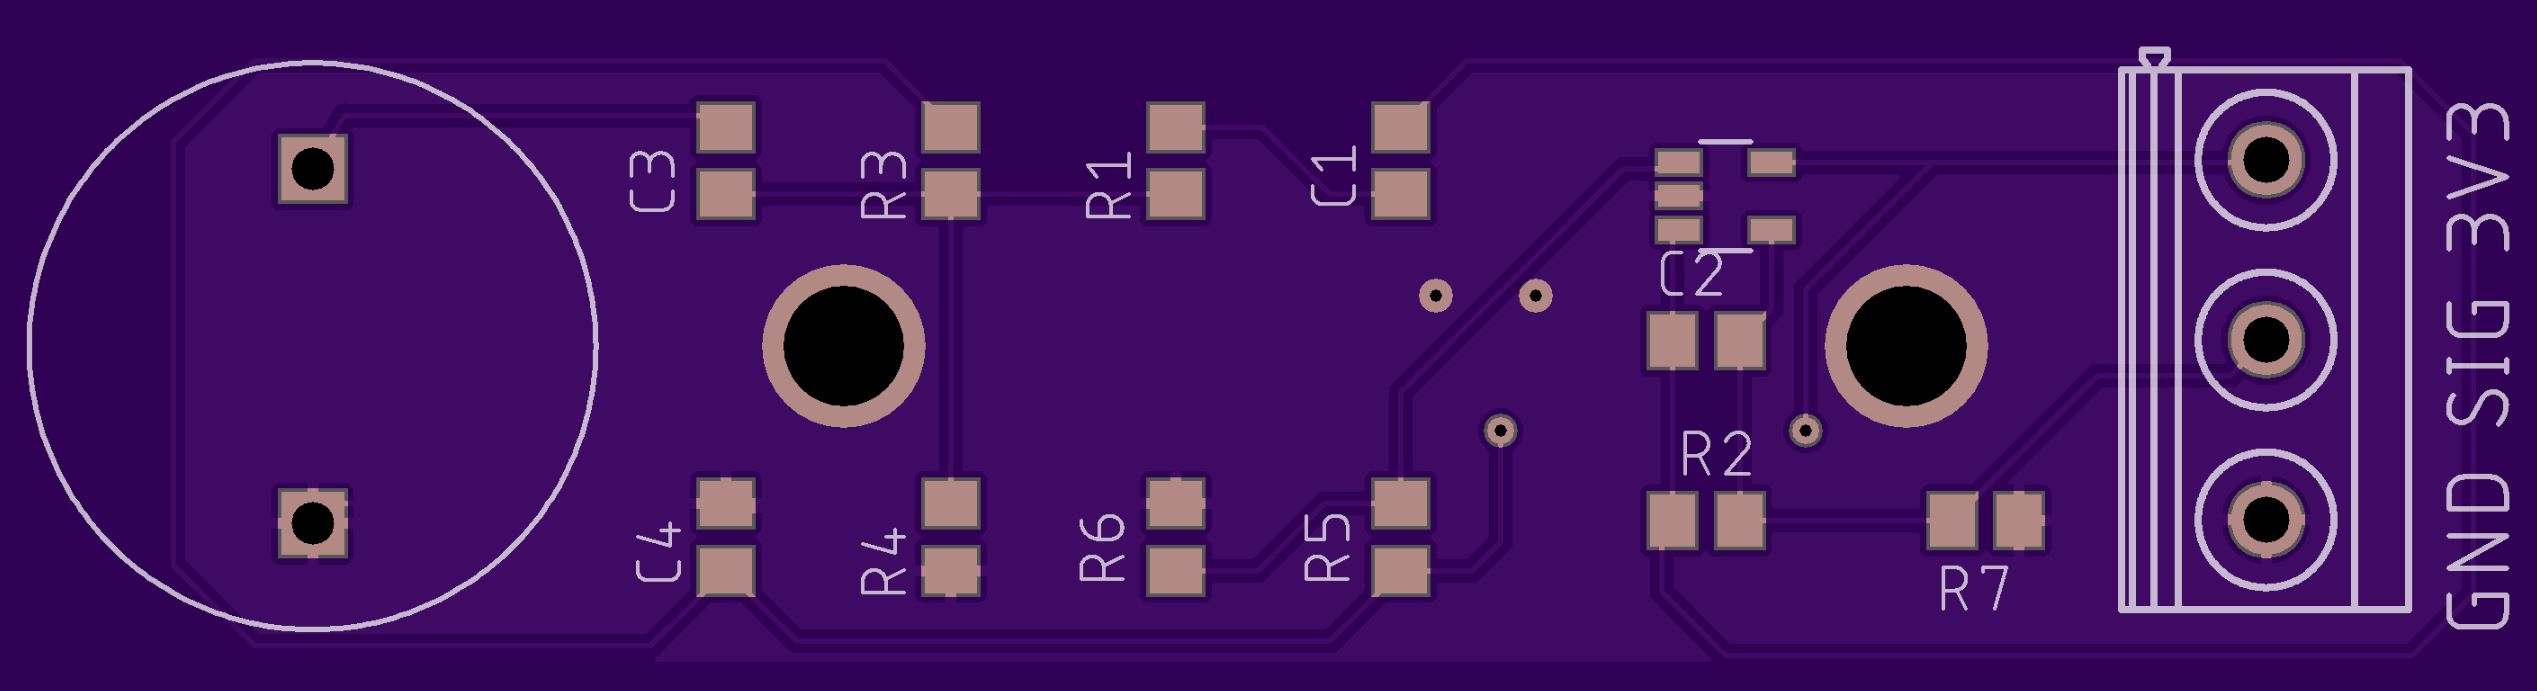
\includegraphics[width=0.7\textwidth]{abpfeagle}
	\caption{Custom active band-pass filter render from OSH Park order}
	\label{fig:abpfeagle}
\end{figure}

\section{Receiver Array and PCB Assembly} \label{sec:3s5}
The assembly process for the iSBL array involved soldering the PCBs and breadboard, assembling the acrylic frame, securing the electrical components to the acrylic frame, and attaching the array to the Fo-SHIP’s end effector.

First, the PCBs were assembled. After being delivered from Mouser, the electrical components were soldered to the PCBs; see Figure \ref{fig:abpfboard} for the PCBs before they were populated with components. All PCBs were hand-soldered using a soldering iron, heat gun, and solder wire. Figure \ref{fig:abpfmanu} shows one PCB in the process of being soldered, and Figure \ref{fig:abpffinished} shows a completed PCB. 

\begin{figure}[htbp]
	\centering
	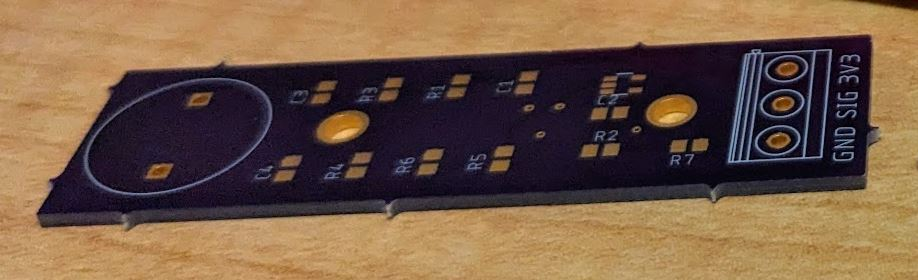
\includegraphics[width=0.7\textwidth]{abpfboard}
	\caption{Fabricated active band-pass filter PCB, unpopulated}
	\label{fig:abpfboard}
\end{figure}

\begin{figure}[htbp]
	\centering
	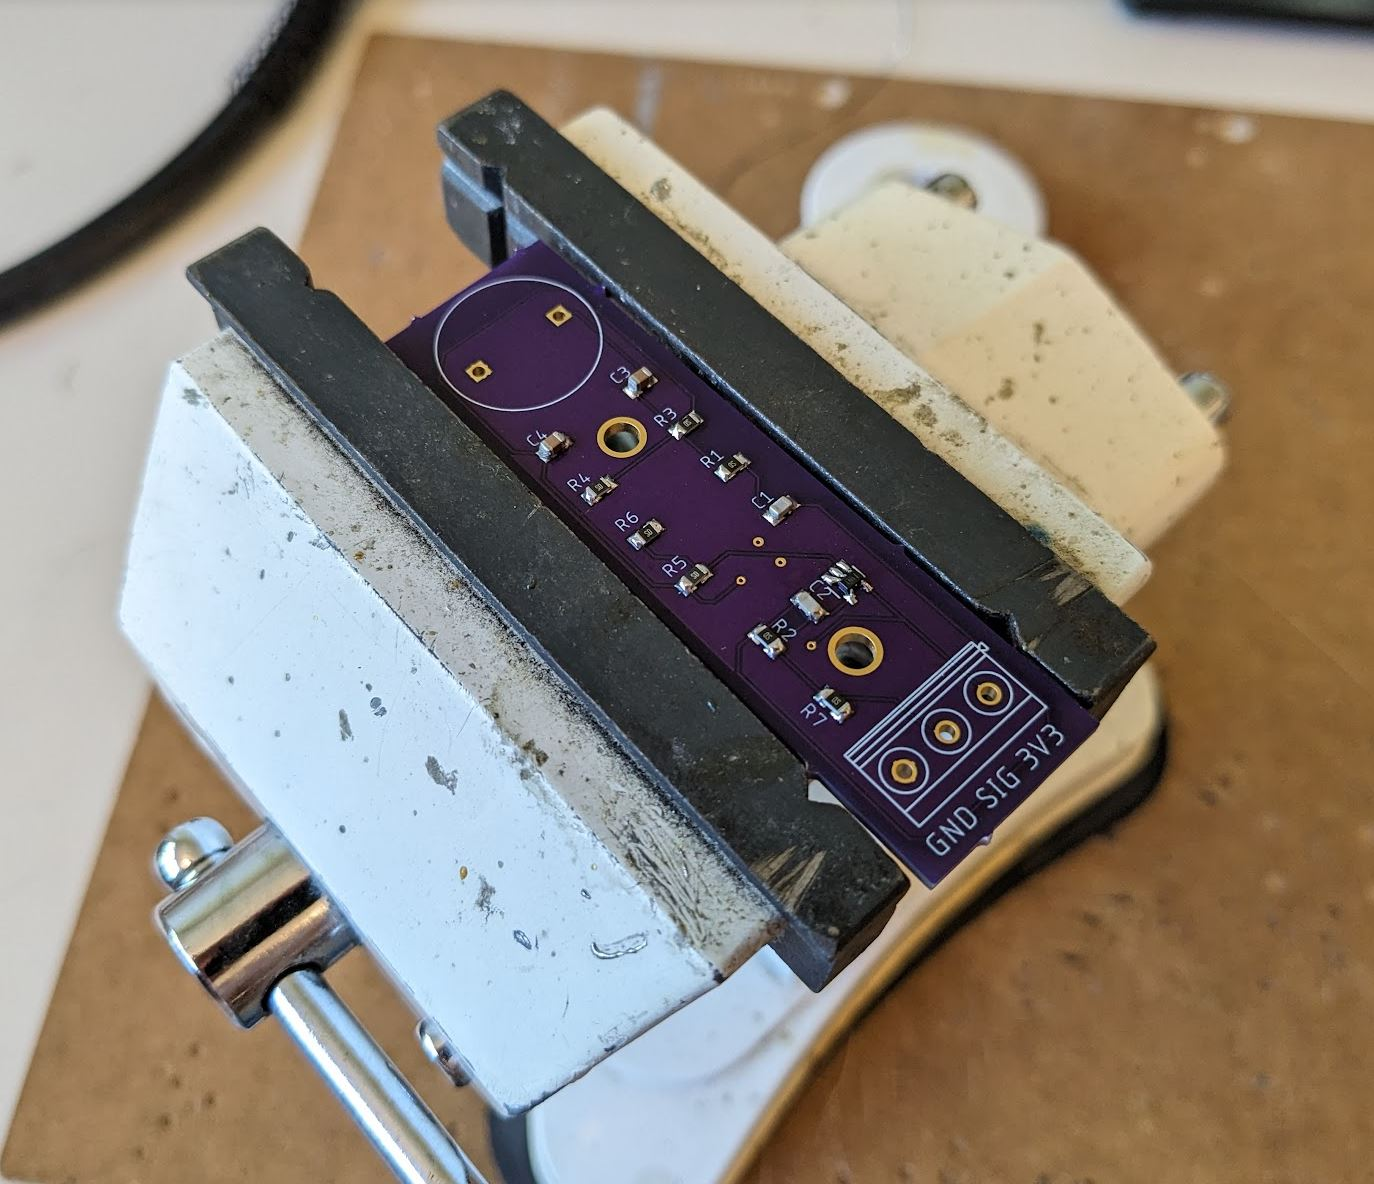
\includegraphics[width=0.58\textwidth]{abpfmanu}
	\caption{Soldering in-progess for PCB}
	\label{fig:abpfmanu}
\end{figure}

\begin{figure}[htbp]
	\centering
	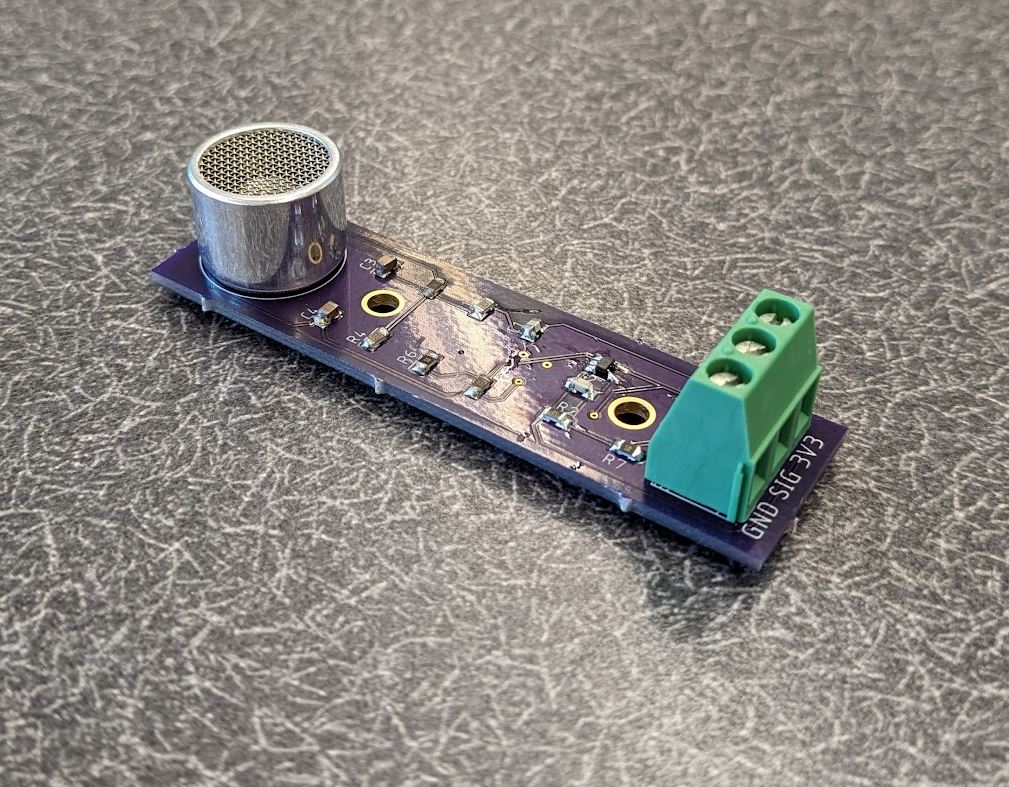
\includegraphics[width=0.58\textwidth]{abpffinished}
	\caption{Fully-assembled active band-pass filter PCB}
	\label{fig:abpffinished}
\end{figure}

After this, the noise-reducing capacitors were soldered to a solderable breadboard. Header pins for each PCB signal line, as well as corresponding wires, were also soldered to the breadboard. Figure \ref{fig:breadboardstm} shows the breadboard. Note that three wires go from the breadboard to each PCB: ground, signal, and 3.3V power.

\begin{figure}[htbp]
	\centering
	\includegraphics[width=0.55\textwidth]{breadboardstm}
	\caption{Soldered breadboard with capacitors, header pins, and wires to ultrasonic receiver PCBs}
	\label{fig:breadboardstm}
\end{figure}

Next, the acrylic frame was assembled using the laser-cut acrylic components, M3x16 screws, and M3 nuts. Spacer plates were sandwiched between the long receiver arm plates and the central hub plates. The receiver PCBs and the soldered breadboard were secured to the acrylic using the M3 screws and nuts. Mounting holes for the IMU and the STM32 development board were not accessible during assembly due to poor planning --- the STM32 is secured to the acrylic hub using cable ties, and the IMU is secured to the acrylic hub plate using adhesive. Two cable tie segments were cut from a single tie and placed on either side of the base of the IMU, and adhesive was placed in the space between the segments. This ensures that the IMU is parallel to the acrylic plate. All wiring connecting the STM32, breadboard, IMU, and receiver PCBs was added; loose wires were secured using cable ties. Lastly, the spacing between the ultrasonic receiver elements and the center was validated to be 25.0cm ± 0.1cm, and the spacing between individual receiver elements was validated to be 35.5cm ± 0.5cm.

The final step of assembly was attaching the iSBL array to the Fo-SHIP end effector. The 3D-printed adapter was secured to the end effector using M3 screws; the iSBL array was secured to the adapter using additional M3 screws and nuts. All connections were tightened in a star pattern to avoid misalignments and to reduce the slop in the system. See Figure \ref{fig:isblfront} for the fully-assembled iSBL array.

\begin{figure}[htbp]
	\centering
	\includegraphics[width=\textwidth]{isblfront}
	\caption{Fully-assembled iSBL array}
	\label{fig:isblfront}
\end{figure}

\section{Transmitter Design} \label{sec:3s6}
The purpose of the transmitter system is to send a particular acoustic pulse towards the receiver array using an ultrasonic transducer. This section details the hardware design of the transmitter, followed by the software design.

\subsection{Transmitter Hardware Design} \label{ssec:3s6s1}
The hardware design of the transmitter was one of the most iterated designs in this entire thesis. The basic design involves a microcontroller for generating a particular pulse, a motor driver (or other driver IC) to control the voltage across an ultrasonic transducer, and an ultrasonic transducer (single or multiple) to transmit the sound towards the receiver array. 

The microcontroller used is an STM32F411CEU6, on a development board commonly referred to as a “BlackPill” \cite{blackpill}. This microcontroller development board has a small form factor, is fairly low cost, and has high performance. Since the only physical connections to the microcontroller were two GPIO pins controlling the motor driver and a ground connection, the form factor was acceptable. Additionally, the microcontroller’s only function would be to generate a waveform (no multitasking), so extremely high performance like the STM32H723ZG provides would not be necessary.

The motor driver went through many iterations before finalizing a design. To work with the 40kHz transducers, it needed to have a switching frequency at or above 80kHz, and needed to provide up to 24Vpp at the voltage output. Initially, spare motor driver ICs were tested and deemed unfit for the purpose: a TPIC0107B motor driver had a switching frequency of 2kHz, far below the 80kHz required; an LM386 audio amplifier had a maximum output voltage of 12Vpp, which was half the maximum of the ultrasonic transducer’s range and did not produce a loud enough signal; an LM18298 motor driver had an adequate maximum output voltage, but only had a switching frequency of 25kHz; and an H-bridge constructed out of only P-type MOSFETs worked but wasted half its output power. Eventually, a spare motor driver made using optical-coupled MOSFETs by Charlie Refvem, one of the members of this thesis committee, was tested and performed fantastically. Many thanks to Charlie for loaning out the motor driver!

Lastly, the ultrasonic transducer chosen for this system is a 400ST160, manufactured by Pro-Wave Electronics Corporation \cite{400sr160}. This transducer has a center frequency of 40kHz and an acceptable beam angle of 55° at half-power. Two transducer configurations were tested: a single transducer, and a 3x3 array of transducers with 2.03cm spacing. The 3x3 array used a single input (all positive legs soldered together, and all negative legs soldered together); a phased array was considered, but was ultimately deemed out-of-scope. The array was simulated in Matlab\textsuperscript{\textregistered}\xspace (see Figure \ref{fig:matlab}) and shows a much shallower beam angle of approximately 7.5° for half-power. Experimentally, the 3x3 array delivered the same amount of acoustic energy at 28ft as a single transmitter did at 10ft; using the inverse square law for sound propagation, the 3x3 array has approximately 7.84x the power of a single transmitter, slightly less than the ideal 9x.

\begin{figure}[htbp]
	\centering
	\includegraphics[width=1\textwidth]{matlab}
	\caption{Matlab simulation of 3x3 array}
	\label{fig:matlab}
\end{figure}

Figure \ref{fig:txnine} shows an image of the fully assembled system, with the 3x3 array connected to the output of the motor driver. Ultimately, the much shallower beam angle of the 3x3 was producing poor results with the receiver array; the transmitter would need to be a minimum of 12.5ft away to hit each receiver element with a half-power pulse. Additionally, the array caused some phasing issues with the multiple transmitter elements, which ultimately produced a slightly different signal at each receiver. Since the acoustic model assumes a single transmitter and an identical (but time-shifted) signal at each receiver, the 3x3 array would not be ideal, and the single transmitter was used for the remainder of the testing for this thesis.

\begin{figure}[htbp]
	\centering
	\includegraphics[width=0.65\textwidth]{txnine}
	\caption{Transmitter system with 3x3 array (eventually swapped with single transmitter)}
	\label{fig:txnine}
\end{figure}

\subsection{Transmitter Software Design} \label{ssec:3s6s2}
The STM32F411CEU6 was programmed using an ST-LINK/V2 from a spare Nucleo board. The code was developed in STM32CubeIDE\textsuperscript{\textregistered}\xspace, a software tool designed for programming STM32 microcontrollers. The code has two main functions: to generate a string of instructions for the motor driver, and to execute those instructions by toggling GPIO pins connected to the motor driver. 

Originally, a planned component of this thesis was to transmit GPS data over ultrasonic audio waves; an 8-bit character would be sent over ultrasonic, encoded using on-off keying, and then decoded using a neural network \cite{ultrann}. However, this was unable to be implemented into the thesis in time for submission. This functionality would allow the transmission of GPS coordinates from the transmitter buoy to the underwater vehicle, and is planned for future implementation.

The first step in the code is generating the instructions for the motor driver. This occurs once per second. An 8-bit character is chosen, converted to its binary representation, and stored in a list. The first six bits of the list are a header; they are meant to trigger the receivers to start recording.

\begin{lstlisting}[language=C++]
message_int ++;			// pick the next number
message_int %= 256;		// between 0 and 255 (8-bit length),
message_char = (char)message_int;		// and save it as a char

// save in the last 8 bits of message_string
for(int i = 8; i > 0; i--){				
	message_string[14-i] = (message_int >> (i-1)) & 1;
}

message_string[0] = 1; 	// initialize the message with a header
message_string[1] = 1;
message_string[2] = 1;
message_string[3] = 1;
message_string[4] = 0;
message_string[5] = 0;
\end{lstlisting}

The \verb|message_string| is a list of 1s and 0s which will be transmitted using ultrasonic pulses --- in a set time frame, one pulse denotes a 1 bit, and no pulse denotes a 0 bit. However, single pulses cannot be used for this case! Since the operating frequency is the same as the resonant frequency of the receivers, sending a single 40kHz wave would produce significant ringing in the transmitters. This ringing would affect data transmission rates if attempting to transmit bits over audio; additionally, sharper impulses provide the best results for time-differencing (as performed in Section \ref{sec:3s8}), so reducing the ringing is a primary concern.

A paper by researchers in the United Kingdom details a method for reducing this ringing by implementing active damping \cite{activedamping}. Figure \ref{fig:activedamping} shows two active damping waveforms and their results compared to a single transmitter pulse. Note that the second waveform produces an 80.7\% decrease in the length of the received pulse.

\begin{figure}[htbp]
	\centering
	\includegraphics[width=1\textwidth]{activedamping}
	\caption{Active damping of ultrasonic receivers using engineered waves \cite{activedamping}}
	\label{fig:activedamping}
\end{figure}


In the paper, the researchers are working with 40.01kHz audio waves. The second waveform shows a delay of 11.75us between sets of waves; these are approximately (but not perfectly) delays of half a wavelength. To simplify implementation, this thesis uses a modified waveform from the researchers’ second waveform: five 40kHz waves, one half-phase delay, six 40kHz waves, one half-phase delay, and three 40kHz waves. 

This modified waveform was implemented in the microcontroller code. The optical sensor motor driver takes in two inputs, A and B. A truth table for the motor driver can be seen in Table \ref{tab:truth} below. The positive lead of the transducer is connected to Out1 and the negative lead is connected to Out2. By holding the same voltage across both leads, the motion of the transducer is halted; by oscillating between the second and third row of the truth table at 80kHz, a 40kHz square-wave can be generated to drive the transducer.

\begin{table}[htbp]
	\centering
	\caption{Truth table for motor driver}
	\label{tab:truth}
	\begin{tabular}{|c|c|c|c|}
		\hline
		Logic level, InA & Logic level, InB & Voltage, Out1 & Voltage, Out2 \\
		\hline
		0 & 0 & 0V & 0V \\
		\hline
		0 & 1 & +12V & 0V \\
		\hline
		1 & 0 & 0V & +12V \\
		\hline
		1 & 1 & +12V & +12V \\
		\hline
	\end{tabular}
\end{table}

In the code, two lists are defined: \verb|on_a_string| provides a list of logic levels for InA, and \verb|on_b_string| provides a list of logic levels for InB. If the GPIO pins connected to these inputs are set to the instructions in these lists at a rate of 80kHz, a square version of the modified waveform is produced. See Figure \ref{fig:modwave} for the waveform produced by the GPIO pins when the code is run. A sinusoidal waveform was attempted and would technically produce better results, but the square waveform can work with a much slower update rate and produced acceptable results at the receiver. Note that trailing ones are set to allow an appropriate delay between subsequent pulses.

\begin{lstlisting}[language=C++]
/**< list of GPIO ODR instructions to send a 1 bit over audio, positive input to motor driver */
uint8_t on_a_string[] = {
	1, 0,
	1, 0,
	1, 0,
	1, 0,
	1, 0,
	1,	
	1, 0,
	1, 0,
	1, 0,
	1, 0,
	1, 0,
	1, 0,
	1,
	1, 0,
	1, 0,
	1, 0,
	1, 1, 1, 1, 1, 1, 1, 1, 1, 1};

/**< list of GPIO ODR instructions to send a 1 bit over audio, negative input to motor driver */
uint8_t on_b_string[] = {
	0, 1,
	0, 1,
	0, 1,
	0, 1,
	0, 1,
	1,
	0, 1,
	0, 1,
	0, 1,
	0, 1,
	0, 1,
	0, 1,
	1,
	0, 1,
	0, 1,
	0, 1,
	1, 1, 1, 1, 1, 1, 1, 1, 1, 1};
\end{lstlisting}

\begin{figure}[htbp]
	\centering
	\includegraphics[width=0.75\textwidth]{modwave}
	\caption{Output of GPIO pins producing square waveform, input to motor driver}
	\label{fig:modwave}
\end{figure}

Now, the \verb|message_string| generated previously is combined with the above strings to produce a list of instructions. This list of instructions, \verb|driver_string|, details what the GPIO port associated with the motor driver pins should set its output data register (ODR) to every 11.25us. For every 1 bit in \verb|message_string|, it fills the \verb|driver_string| with the instructions in \verb|on_a_string| and \verb|on_b_string|. For every 0 bit in \verb|message_string|, it fills the \verb|driver_string| with an equivalent number of zeros. The code assumes that InA is connected to pin B6 and InB is connected to pin B7 on the STM32F411CEU6.

\begin{lstlisting}[language=C++]
int index = 0;
for (int i = 0; i < sizeof(message_string); i++) {
	if (message_string[i] == 1) {
		for (int j = 0; j < sizeof(on_a_string); j++) {
			driver_string[index] = (on_a_string[j] << 6) | (on_b_string[j] << 7);
			index++;
		}
	} else {
		for (int j = 0; j < sizeof(on_a_string); j++) {
			driver_string[index] = 0;
			index++;
		}
	}
}
\end{lstlisting}

After the message is generated, a timer is started that updates at 80kHz. Every update, the GPIO ODR is set to the next value of \verb|driver_string|. Since each message bit takes 40 cycles of an 80kHz timer to send, the effective data rate of the transmission is approximately 2kHz. This means that in an ideal environment, data can be sent from the transmitter to the receiver at 2kb/s. Figure \ref{fig:oscope11110001} shows the 8-bit number 241, represented in binary as 11110001, as received by the iSBL receiver array.

\begin{lstlisting}[language=C++]
if (htim->Instance == TIM4){
	GPIOB->ODR = driver_string[instruction_counter]; 
	instruction_counter++;
	if (instruction_counter >= DRIVER_STRING_LEN){
		instruction_counter = 0;
		HAL_TIM_Base_Stop(&htim4);
	}
}
\end{lstlisting}

\begin{figure}[htbp]
	\centering
	\includegraphics[width=0.75\textwidth]{oscope11110001}
	\caption{8-bit number 241 (11110001) transmitted over ultrasonic}
	\label{fig:oscope11110001}
\end{figure}

This process repeats once per second. Though the transmitter sends a message with multiple individual 40kHz pulses and 14 data bits, the transmission sent every second will be referred to as “a single acoustic pulse” for the remainder of this paper.

\section{Recording an Audio Pulse} \label{sec:3s7}
This section is the first of three detailing the acoustic position estimate code running on the STM32H723ZG, referred to as ``the STM32" in this paper. This first section details the overall finite-state machine diagram for the system, how the ADC is configured for MultiMode, the two different recording states (triggering and full recording), and how a “good” pulse is determined.

\subsection{Finite-State Machine} \label{ssec:3s7s1}
Figure \ref{fig:isblfsm} shows the finite-state machine representation of this system. There are five main states: initialization, triggering, full recording, recording validation, and data processing.

\begin{figure}[htbp]
	\centering
	\includegraphics[width=\textwidth]{isblfsm}
	\caption{Finite-state machine diagram for acoustic positioning system}
	\label{fig:isblfsm}
\end{figure}

In the initialization state, three timers are started: TIM13 is used to count the time between Madgwick filter updates (see Section \ref{sec:4s4}), TIM14 is used to count the time between acoustic position updates (see Section \ref{sec:5s2}), and TIM3 is used to trigger ADC conversions (see Section \ref{ssec:3s7s2}). In this state, the first ADC conversion is started and the system moves into the triggering state.

In the triggering state, a small number of samples are recorded from each microphone (64, in this implementation). These samples are tested to see if they exceed a threshold defined by \verb|TRIG_THRES|. If more than one microphone exceeds the threshold, then the system moves to the full recording state. Otherwise, the system re-enters the triggering state. This state is crucial for detecting the header bits of an acoustic pulse and triggering the full recording process; without this step, a total of 2048 samples per microphone would need to be checked constantly. See Section \ref{ssec:3s7s3} for details on the triggering state.

In the full recording state, 2048 samples are recorded from each microphone (roughly 2.4ms of recording time, which is a good portion of a full 7ms acoustic pulse). The system does not update the IMU during this state to prevent any signal interference or cross-talk. After the recording buffer is full, the system transitions to the recording validation state.

In the recording validation state, the mean and standard deviation of each microphone’s signal is calculated. If all the standard deviations exceed \verb|TRIG_THRES| and the IMU has initialized, then the system moves to the data processing state. If either of these conditions are not met, the system re-enters the triggering state. See Section \ref{ssec:3s7s4} for details on the full recording and recording validation states.

In the data processing state, a position estimate is formed. First, the time shift between the microphone signals is calculated using FFT cross-correlation (see Section \ref{sec:3s8}). Next, the position of each microphone in the acoustic array is rotated by the current orientation of the platform (see Section \ref{ssec:3s9s1}) Then, the position of the transmitter relative to the receiver array is estimated using Hooke-Jeeves search using an acoustic propagation model (see Section \ref{ssec:3s9s2}). This relative position estimate is combined with the known position of the transmitter to give a position estimate of the receiver array (see Section \ref{ssec:3s9s3}). Finally, the acoustic position estimate and the dead reckoning position estimate are combined using Kalman filters (see Chapter \ref{chap:5c}).

In the background, linear acceleration, angular velocity, and magnetic field strength data are being recorded from the IMU at 208Hz. This data is then converted into an orientation estimate using a Madgwick filter, and into a change-in-position estimate using dead reckoning. See Chapter \ref{chap:4c} for details.

\subsection{ADC Configuration} \label{ssec:3s7s2}
The sampling rate of the ADC determines the resolution of the time shift calculation. The time shift between two signals sampled at 80kHz can only be determined to within 12.5us; assuming audio signals in water with a speed of sound of 1500 m/s \cite{computational}, this means that the distance from each microphone to the transmitter can only be discerned to within 9.4mm. This shift is enough to introduce significant error into the position estimation algorithm, so increasing the sampling rate of the ADC is a primary concern.

The ADC has multiple resolutions to choose from (8-bit, 12-bit, 16-bit, etc.). After testing, 12-bit resolution was found to provide enough resolution for the filtered audio signals with a resolution of approximately 0.81mV per bit. A single 12-bit ADC conversion takes approximately 12.5 cycles to convert on the STM32 \cite{stmdatasheet}, and higher resolutions take even longer.

Due to the input impedance of the active band-pass filter PCBs, additional ADC cycles were needed to stabilize the voltage output of the filter PCBs. Different sampling times were tested, and 8.5 cycles per conversion was found to provide a stable signal without requiring excess sampling time. Running at the maximum ADC clock speed of 50MHz and combining the standard conversion time of 12.5 cycles with the additional sampling time of 8.5 cycles, it takes approximately 0.42us to complete a single ADC conversion for one microphone.

Initially, only one ADC on the microcontroller was used for all four microphones. When the timer TIM3 updated, it would trigger a series of four subsequent conversions, one from each microphone. See Figure \ref{fig:adctimingsingle} for a timing diagram of these conversions. Since all four conversions happened subsequently, the maximum theoretical sampling rate for the ADC was approximately 595kHz. In practice, 500kHz was the maximum possible sampling rate --- anything above this rate produced incomplete conversions for the final channel.

\begin{figure}[htbp]
	\centering
	\includegraphics[width=\textwidth]{adctimingsingle}
	\caption{Timing diagram for four subsequent ADC conversions \cite{stmdatasheet}}
	\label{fig:adctimingsingle}
\end{figure}

However, using a configuration called MultiMode (also called ``dual ADC" mode) allows the sampling rate to be doubled. In this configuration, one ADC (ADC1) is designated as the primary ADC, and a different ADC (ADC2) is designated as the secondary ADC. When the primary ADC is triggered, it then automatically triggers the second ADC to start recording 1.5 cycles later \cite{stmdatasheet}. Both the primary and secondary ADC use two channels; ADC1 reads from microphones 0 and 2, and ADC2 reads from microphones 1 and 3. See Figure \ref{fig:adctimingmulti} for a timing diagram of this MultiMode configuration. Note that the figure shows two ADCs running in MultiMode with four channels each; the thesis implementation uses two ADCs with only two channels each.

\begin{figure}[htbp]
	\centering
	\includegraphics[width=0.75\textwidth]{adctimingmulti}
	\caption{Timing diagram for MultiMode ADC conversions \cite{stmdatasheet}}
	\label{fig:adctimingmulti}
\end{figure}

Since MultiMode uses two ADCs running simultaneously (with a 1.5 cycle delay), the maximum theoretical sampling rate for the primary ADC is approximately 1.15MHz. In practice, 851.4kHz was the maximum possible sampling rate --- anything above this rate produced incomplete conversions on the final two channels.

After conversion, the ADC readings must be saved in a data buffer. Manually writing them to the buffer would significantly impact the maximum allowed sampling rate, so direct memory access (DMA) is used. A DMA stream is configured to write the ADC conversions to a memory buffer; however, using MultiMode requires special handling of these conversions. In normal modes, the 12-bit ADC conversions are stored as \verb|uint16_t| values. MultiMode saves simultaneous readings as \verb|uint32_t| values, with the first conversion (ADC1) stored in the first 16 bits of the \verb|uint32_t| value and the second (ADC2) stored in the last 16 bits of the \verb|uint32_t| value. Two macros were created to extract the individual ADC readings from these values. The code snippet below shows these two macros, as well as the initialization sequence for the ADCs in the initialization state.

\begin{lstlisting}[language=C++]
#define adc1conv(data) ((data) & 0xFFFF)
#define adc2conv(data) ((data >> 16) & 0xFFFF)
...
// start DMA from ADCs, writing TRIG_BUF_LEN samples to trig_buf (triggering state)
HAL_ADC_Start(&hadc2);
HAL_ADCEx_MultiModeStart_DMA(&hadc1, (uint32_t*)trig_buf, TRIG_BUF_LEN * NUM_MIC / 2);
// start timer that controls ADCs
HAL_TIM_Base_Start_IT(&htim3);
\end{lstlisting}

\subsection{Triggering State} \label{ssec:3s7s3}
The triggering state is used to decide if an acoustic pulse is incoming. In this state, the ADC records 64 samples from each microphone at 851.4kHz and saves their values to the buffer \verb|trig_buf|. Once the ADC conversion is finished and all readings are saved to the buffer, the recordings from each individual microphone are extracted from the buffer and the mean of each signal is calculated.

\begin{lstlisting}[language=C++]
float mic0_mean = 0, mic1_mean = 0, mic2_mean = 0, mic3_mean = 0;
for (int i = 0; i < TRIG_BUF_LEN * NUM_MIC/2; i += NUM_MIC/2) {
	mic0_mean += (float)adc1conv(trig_buf[i]);
	mic1_mean += (float)adc2conv(trig_buf[i]);
	mic2_mean += (float)adc1conv(trig_buf[i+1]);
	mic3_mean += (float)adc2conv(trig_buf[i+1]);
}
mic0_mean /= (float)TRIG_BUF_LEN;
mic1_mean /= (float)TRIG_BUF_LEN;
mic2_mean /= (float)TRIG_BUF_LEN;
mic3_mean /= (float)TRIG_BUF_LEN;
\end{lstlisting}

Next, the program checks if any of the microphones have recorded signals with sufficient variance. If any five subsequent values in a microphone’s signal exceed \verb|TRIG_THRES|, then that microphone has registered a significant signal. The code loops through every set of five values in each microphone’s signal and determines if any of the sets contain values all greater than \verb|TRIG_THRES|. If they do, then the flag \verb|exceedsThresholdmicN| is set to 1 for that microphone. This provides a robust method for determining when to record a full signal. For a 40kHz wave sampled at 851.4kHz, there are approximately 21 samples per full waveform; checking for five samples in a row detects the peaks of these waveforms when recording only a small number of samples.

\begin{lstlisting}[language=C++]
#define NUM_THRES_ROW 5
...
int exceedsThresholdmic0 = 0;
int exceedsThresholdmic1 = 0;
int exceedsThresholdmic2 = 0;
int exceedsThresholdmic3 = 0;
int loopLen = TRIG_BUF_LEN - NUM_THRES_ROW;
for (int i = 0; i < loopLen; i += 1) {
	int thres_count_mic0 = 0;
	int thres_count_mic1 = 0;
	int thres_count_mic2 = 0;
	int thres_count_mic3 = 0;
	
	// check if the next NUM_THRES_ROWS values exceed TRIG_THRES
	for (int t = 0; t < NUM_THRES_ROW; t++) {
		thres_count_mic0 += fabsf((float)adc1conv(trig_buf[i*NUM_MIC/2 + t*NUM_MIC/2 + 0]) - mic0_mean) > TRIG_THRES;
		thres_count_mic1 += fabsf((float)adc2conv(trig_buf[i*NUM_MIC/2 + t*NUM_MIC/2 + 0]) - mic1_mean) > TRIG_THRES;
		thres_count_mic2 += fabsf((float)adc1conv(trig_buf[i*NUM_MIC/2 + t*NUM_MIC/2 + 1]) - mic2_mean) > TRIG_THRES;
		thres_count_mic3 += fabsf((float)adc2conv(trig_buf[i*NUM_MIC/2 + t*NUM_MIC/2 + 1]) - mic3_mean) > TRIG_THRES;
	}
	
	if (thres_count_mic0 == NUM_THRES_ROW) exceedsThresholdmic0 = 1;
	if (thres_count_mic1 == NUM_THRES_ROW) exceedsThresholdmic1 = 1;
	if (thres_count_mic2 == NUM_THRES_ROW) exceedsThresholdmic2 = 1;
	if (thres_count_mic3 == NUM_THRES_ROW) exceedsThresholdmic3 = 1;
	
	// If all mics have been exceeded, we can break the loop
	if (exceedsThresholdmic0 && exceedsThresholdmic1 && exceedsThresholdmic2 && exceedsThresholdmic3) {
		break;
	}
}
\end{lstlisting}

After this, the total number of microphone signals that have met the threshold criteria is summed. If more than one microphone meets the threshold criteria, then the system transitions to the full recording state. Otherwise, the triggering state restarts and the above process repeats. In this state, each microphone has an associated LED for debugging; if the LED for a microphone lights up, then that microphone’s signal exceeded the threshold. This was crucial for ensuring the transmitter was pointing directly at the acoustic array during the data collection in Chapter \ref{chap:6c}.

\begin{lstlisting}[language=C++]
int exceedsThreshold = exceedsThresholdmic0 + exceedsThresholdmic1 + exceedsThresholdmic2 + exceedsThresholdmic3;

// if at least two microphones exceeded the threshold, move to the full recording state
if (exceedsThreshold > 1) {
	state = 2;                // transition to full recording state
	recording = 1;            // prevent interrupting ADC recording
	HAL_ADC_Start(&hadc2);    // start the secondary ADC
	HAL_ADCEx_MultiModeStart_DMA(&hadc1, (uint32_t*)adc_buf, ADC_BUF_LEN * NUM_MIC / 2); // start the primary ADC in DMA mode
	
	// otherwise, restart the triggering process
} else {
	HAL_ADC_Start(&hadc2);    // start the secondary ADC
	HAL_ADCEx_MultiModeStart_DMA(&hadc1, (uint32_t*)trig_buf, TRIG_BUF_LEN * NUM_MIC / 2); // start the primary ADC in DMA mode
}
\end{lstlisting}

\subsection{Full Recording and Recording Validation State} \label{ssec:3s7s4}
Not much happens during the full recording state besides ADC conversions. In this state, the STM32 halts reading from the IMU and updating the Madgwick filter. Even though the ADC conversions happen in the background and are written to a memory buffer using DMA, it is imperative that the ADC sampling occurs at the maximum sampling rate; so, any potential sources of noise or resource use are halted.

Once the ADC conversion is finished and 2048 samples are recorded from each microphone, the system transitions to the recording validation state. This state is similar to the triggering state: its objective is to determine if the recording has enough variance to accurately perform a time shift calculation. Unlike the triggering state, a different method is used for determining the quality of the signal. The vast length of the full recording signals means that the standard deviation can be used as a good metric for the signal variance; it is assumed, due to the filtering of non-40kHz signals and amplification of 40kHz signals, that a signal with a sufficiently large standard deviation contains the acoustic pulse from the transmitter.

First, the mean and standard deviation of each signal is calculated. If the standard deviation of all four signals exceeds \verb|TRIG_THRES| and the IMU has been initialized, then the recording is considered sufficient for further data processing and the system transitions to the data processing state. If any of the signals fails to exceed the threshold, then the system returns to the triggering state; if this is the case, then the ADC buffers are reset. 

\begin{lstlisting}[language=C++]
// set recording flag to 0 because the ADC has stopped recording
recording = 0;

// stop the ADC trigger timer
HAL_TIM_Base_Stop_IT(&htim3);

// variables for calculating average and standard deviation for each microphone
mic0_avg = 0, mic1_avg = 0, mic2_avg = 0, mic3_avg = 0;
mic0_var = 0, mic1_var = 0, mic2_var = 0, mic3_var = 0;
mic0_stdev = 0, mic1_stdev = 0, mic2_stdev = 0, mic3_stdev = 0;

// calculate average of each mic signal
for (int i = 0; i < ADC_BUF_LEN * NUM_MIC / 2; i += NUM_MIC / 2) {
	mic0_avg += (float)adc1conv(adc_buf[i]);
	mic1_avg += (float)adc1conv(adc_buf[i+1]);
	mic2_avg += (float)adc2conv(adc_buf[i]);
	mic3_avg += (float)adc2conv(adc_buf[i+1]);
}
mic0_avg /= (float)ADC_BUF_LEN;
mic1_avg /= (float)ADC_BUF_LEN;
mic2_avg /= (float)ADC_BUF_LEN;
mic3_avg /= (float)ADC_BUF_LEN;

// calculate variance of each mic
for (int i = 0; i < ADC_BUF_LEN * NUM_MIC / 2; i += NUM_MIC / 2) {
	mic0_var += powf((float)adc1conv(adc_buf[i]) - mic0_avg, 2);
	mic1_var += powf((float)adc1conv(adc_buf[i+1]) - mic1_avg, 2);
	mic2_var += powf((float)adc2conv(adc_buf[i]) - mic2_avg, 2);
	mic3_var += powf((float)adc2conv(adc_buf[i+1]) - mic3_avg, 2);
}
mic0_var /= (float)(ADC_BUF_LEN - 1);
mic1_var /= (float)(ADC_BUF_LEN - 1);
mic2_var /= (float)(ADC_BUF_LEN - 1);
mic3_var /= (float)(ADC_BUF_LEN - 1);

// calculate standard deviation of each mic
mic0_stdev = sqrtf(mic0_var);
mic1_stdev = sqrtf(mic1_var);
mic2_stdev = sqrtf(mic2_var);
mic3_stdev = sqrtf(mic3_var);

// check if each microphone exceeds the threshold for "good" data
int stdev_above_thres = 0;
stdev_above_thres += mic0_stdev > (TRIG_THRES);
stdev_above_thres += mic1_stdev > (TRIG_THRES);
stdev_above_thres += mic2_stdev > (TRIG_THRES);
stdev_above_thres += mic3_stdev > (TRIG_THRES);

// if the signal is good and the initial IMU angle has been set (remove yaw), then
// move to the data processing state
if ((stdev_above_thres >= NUM_MIC) && imu_init_set){
	state = 4;
}
else{
	// reset all ADC buffers
	memset(adc_buf, 0, sizeof(adc_buf));
	memset(trig_buf, 0, sizeof(trig_buf));
	...
	// return to the trigger state
	state = 1;
	
	// restart the DMA from ADCs and the timer that controls the ADCs
	HAL_ADC_Start(&hadc2);
	HAL_ADCEx_MultiModeStart_DMA(&hadc1, (uint32_t*)trig_buf, TRIG_BUF_LEN * NUM_MIC / 2);
	HAL_TIM_Base_Start_IT(&htim3);
}
\end{lstlisting}

Figure \ref{fig:oscope4} shows an acoustic pulse recorded from four microphones on a Keysight oscilloscope. Figure \ref{fig:adc4} shows an acoustic pulse (with a slightly different receiver orientation) recorded using the STM32 and ADCs. In that figure, the ADC readings have been normalized, as described in Section \ref{ssec:3s8s2}. The ADC readings tend to be slightly noisier than the oscilloscope readings, but are sufficient for calculating time shifts.

\begin{figure}[htbp]
	\centering
	\includegraphics[width=0.75\textwidth]{oscope4}
	\caption{Microphone recordings on Keysight oscilloscope}
	\label{fig:oscope4}
\end{figure}

\begin{figure}[htbp]
	\centering
	\includegraphics[width=0.75\textwidth]{adc4}
	\caption{Microphone recordings on STM32 ADCs, slightly different receiver orientation}
	\label{fig:adc4}
\end{figure}

\section{Calculating Time Shift} \label{sec:3s8}
Once a pulse has been recorded from all four microphones, the time shift between microphone recordings is calculated. Cross-correlations are a standard method for computing the time shift between two similar signals, but this method can be quite computationally-taxing  for large signals; for this reason, the fast Fourier transform (FFT) cross-correlation method is used. This takes the computation time from \(O(n^2)\) time to \(O(n \times log(n))\) time \cite{dspguide}. This section describes the theory of the FFT cross-correlation, then shows its implementation on the microcontroller.

\subsection{FFT Cross-Correlation Theory} \label{ssec:3s8s1}
Before the FFT cross-correlation can be understood, the basics of the convolution operation must be discussed. Cross-correlation and convolution are effectively the same operation, but with one of the signals flipped horizontally.

The convolution is a mathematical operation that takes two signals and produces a third signal \cite{dspguide}. The mathematical notation for a convolution of discrete signals is:

\begin{equation} \label{eq:3eq1}
	x[n] * h[n] = y[n]
\end{equation}

Figure \ref{fig:convxn} shows an example convolution, while Figure \ref{fig:convexp} shows the components that make up the output of the convolution. A convolution operation can be thought of as flipping the second signal horizontally and then sliding it over the first signal, summing the shared area underneath both signals. Figure \ref{fig:convandcross} gives a wonderful visualization of the process, and the \href{https://en.wikipedia.org/wiki/Cross-correlation#/media/File:Cross_correlation_animation.gif}{\ul{GIF on the Wikipedia page for cross-correlation}} is a fantastic animation showing how the cross-correlation of two signals is computed. 

\begin{figure}[htbp!]
	\centering
	\includegraphics[width=.85\textwidth]{convxn}
	\caption{Convolution operation for two discrete signals \cite{dspguide}}
	\label{fig:convxn}
\end{figure}

\begin{figure}[htbp!]
	\centering
	\includegraphics[width=.95\textwidth]{convexp}
	\caption{Convolution operation for two discrete signals, step-by-step process \cite{dspguide}}
	\label{fig:convexp}
\end{figure}

\begin{figure}[htbp]
	\centering
	\includegraphics[width=0.65\textwidth]{convandcross}
	\caption{Convolution and cross-correlation operation for continuous signals \cite{wikicross}}
	\label{fig:convandcross}
\end{figure}

The convolution operation can be used to find the time shift between two similar signals. By first flipping the second signal horizontally (to negate the flip from the convolution operation), the two signals can be convolved to effectively slide them over each other. This process of flipping the second signal prior to the convolution is called cross-correlation. In the output of the cross-correlation, the largest positive value corresponds to the shift between the signals \cite{dspguide}. This should make sense graphically; when the two signals fully overlap, the peaks of both align and the area under the curve shared between the signals is at a maximum. Figure \ref{fig:crosscorrex} shows this for two triangular pulses, with the shift between the two being correctly estimated as -0.5 (signal 2 lags signal 1 by 0.5 time units).

\begin{figure}[htbp]
	\centering
	\includegraphics[width=.90\textwidth]{crosscorrex}
	\caption{Cross-correlation of two triangular pulses}
	\label{fig:crosscorrex}
\end{figure}

When computing the convolution, it is important to add “padding zeros” to the end of both signals. Without this step, the convolution operation is unable to fully “slide” the two signals over each other; it would instead wrap around to the beginning of the signal to complete the operation, which would give an incorrect result. For two signals of equal length \(n\), a total of \(n\) padded zeros should be added to each signal \cite{dspguide}.

The standard convolution operation is very computationally-expensive for long signals, with a convolution of two signals of equal length \(n\) taking \(O(n^2)\) time. However, convolution in the time domain corresponds to multiplication in the frequency domain, which is a much more efficient operation \cite{dspguide}. This changes the computation time for those same signals to \(O(n \times log(n))\) time. For signals of length 4096 (as this implementation uses, more details in next subsection), moving the operation to the frequency domain decreases the number of arithmetic operations required by approximately 99.9\%!

The name of this operation is the FFT convolution, or high-speed convolution. Figure \ref{fig:fftconvtheory} shows a graphical explanation for the operation. Both signals are converted from the time domain to the frequency domain using the FFT operation, multiplied in the frequency domain, and then the product is converted back to the time domain using the inverse FFT operation. For more details on the FFT and inverse FFT, see Chapter 12 of \textit{The Scientist and Engineer’s Guide to Digital Signal Processing} \cite{dspguide}. 

\begin{figure}[htbp]
	\centering
	\includegraphics[width=0.9\textwidth]{fftconvtheory}
	\caption{FFT convolution visual guide \cite{dspguide}}
	\label{fig:fftconvtheory}
\end{figure}

Complex multiplication is required for the frequency domain; signals in that domain have both a real and imaginary component. Complex multiplication is carried out as shown below \cite{dspguide}:

\begin{equation} \label{eq:3eq2}
	(a + bj) (c + dj) = (ac - bd) + j(bc + ad)
\end{equation}

Finally, to perform FFT cross-correlation instead of FFT convolution, two approaches can be taken. First, the second signal can be flipped horizontally. Second, the complex conjugate of the second signal’s FFT transform can be taken. These operations are equivalent; one is in the time domain, and one is in the frequency domain. For this implementation, the complex conjugate operation is chosen, and its definition can be seen below \cite{dspguide}:

\begin{equation} \label{eq:3eq3}
	conj(a + bj) = (a - bj)
\end{equation}

\subsection{FFT Cross-Correlation Implementation} \label{ssec:3s8s2}
The STM32 implementation makes heavy use of the \verb|arm_math.h| digital signal processing library \cite{arm}. This library implements all of the operations described in the previous section and many more. It is written for ARM Cortex M0, M3, M4, and M7 cores; the STM32H723ZG uses a Cortex M7 core. This subsection will walk through the code implementation of the FFT cross-correlation, used in \verb|calculate_time_shift()|.

Once the system transitions to the data processing state, the first step is to normalize the signals from each of the four microphones. Then, the function \verb|calculate_time_shift()| is run on each unique pair of microphone signals; all signals are compared to microphone 0 for simplicity. In future implementations, designing the program to compare the signals to the “best” signal (highest standard deviation, least background noise) would be ideal.

\begin{lstlisting}[language=C++]
// buffers for holding normalized microphone buffers
float32_t mic0_buf[ADC_BUF_LEN];
float32_t mic1_buf[ADC_BUF_LEN];
float32_t mic2_buf[ADC_BUF_LEN];
float32_t mic3_buf[ADC_BUF_LEN];

// de-interleave the ADC values and normalize the data
int index = 0;
for (int i = 0; i < ADC_BUF_LEN * NUM_MIC / 2; i += NUM_MIC / 2) {
	mic0_buf[index] = (((float)adc1conv(adc_buf[i]) - mic0_avg) / mic0_stdev);
	mic1_buf[index] = (((float)adc1conv(adc_buf[i+1]) - mic1_avg) / mic1_stdev);
	mic2_buf[index] = (((float)adc2conv(adc_buf[i]) - mic2_avg) / mic2_stdev);
	mic3_buf[index] = (((float)adc2conv(adc_buf[i+1]) - mic3_avg) / mic3_stdev);
	index += 1;
}

// calculate time-shifts between mic0 and all other microphones
measured_time_shifts[0] = calculate_time_shift(mic0_buf,mic1_buf);
measured_time_shifts[1] = calculate_time_shift(mic0_buf,mic2_buf);
measured_time_shifts[2] = calculate_time_shift(mic0_buf,mic3_buf);
\end{lstlisting}

Separately, a handler for the FFT operations used in \verb|arm_math.h| is initialized in the initialization state of the program. This handler defines the length of buffers used in these operations and must be a power of two. More details for the initialization can be found in the \verb|arm_math.h| documentation \cite{arm}.

\begin{lstlisting}[language=C++]
arm_rfft_fast_init_f32(&fftHandler, FFT_BUF_LEN);
\end{lstlisting}

The time shift function takes in pointers to two data buffers as inputs. These buffers contain the normalized data from two microphone signals. First, the microphone signals are moved into temporary buffers; padded zeros equal to the length of each signal are added. Then, the real FFT of each signal is computed (since both signals only contain real values, not complex). For memory efficiency, some buffers are reused.

\begin{lstlisting}[language=C++]
#define ADC_BUF_LEN 2048
#define FFT_BUF_LEN ADC_BUF_LEN*2
...
float32_t calculate_time_shift(float32_t *micA_buf, float32_t *micB_buf) {
	// load buffers
	float32_t fftBufIn[FFT_BUF_LEN];    /**< input to FFT */
	float32_t fftBuf1Out[FFT_BUF_LEN];  /**< output of first FFT */
	float32_t fftBuf2Out[FFT_BUF_LEN];  /**< output of second FFT */
	float32_t ifftBufIn[FFT_BUF_LEN];   /**< input to inverse FFT */
	float32_t ifftRealOut[FFT_BUF_LEN]; /**< output of inv FFT */
	
	// reset buffers to 0
	memset(fftBufIn, 0, sizeof(fftBufIn));
	memset(fftBuf1Out, 0, sizeof(fftBuf1Out));
	memset(fftBuf2Out, 0, sizeof(fftBuf2Out));
	memset(ifftBufIn, 0, sizeof(ifftBufIn));
	memset(ifftRealOut, 0, sizeof(ifftRealOut));
	
	// load micA values into fftBufIn (remaining values zeros for zero-padding)
	memcpy(fftBufIn, micA_buf, ADC_BUF_LEN * sizeof(float32_t));
	
	// perform real fft on zero-padded micA values
	arm_rfft_fast_f32(&fftHandler, fftBufIn, fftBuf1Out, 0);
	
	// reset fftBufIn
	memset(fftBufIn, 0, sizeof(fftBufIn));
	
	// load micB values into fftBufIn (remaining values zeros for zero-padding)
	memcpy(fftBufIn, micB_buf, ADC_BUF_LEN * sizeof(float32_t));
	
	// perform real fft on zero-padded micB values, put result into temp buf
	arm_rfft_fast_f32(&fftHandler, fftBufIn, ifftBufIn, 0);
\end{lstlisting}

Next, the complex conjugate of the second signal’s FFT is taken. The FFT of the first signal and the complex conjugate of the second signal’s FFT are then multiplied using complex multiplication. Finally, the inverse real FFT of the product is taken (to return only real values, not complex) and stored in a buffer.

\begin{lstlisting}[language=C++]
	// calculate complex conjugate of micB real fft output (required for cross-correlation)
	arm_cmplx_conj_f32(ifftBufIn, fftBuf2Out, FFT_BUF_LEN);
	
	// reset temporary buf
	memset(ifftBufIn, 0, sizeof(ifftBufIn));
	
	// complex multiplication of the two fft output bufs
	arm_cmplx_mult_cmplx_f32(fftBuf1Out, fftBuf2Out, ifftBufIn, FFT_BUF_LEN);
	
	// perform inverse real fft on multiplication result
	arm_rfft_fast_f32(&fftHandler, ifftBufIn, ifftRealOut, 1);
\end{lstlisting}

The results in the inverse FFT output buffer are the output of the FFT cross-correlation operation. To find the most likely time shift between the signals, the index of the largest positive value is found.

\begin{lstlisting}[language=C++]
	// find argmax(ifft_output) to find time shift between signals
	int maxIndex = 0;
	float32_t maxVal = 0.0f;
	for (int i = 0; i < FFT_BUF_LEN; i++) {
		float32_t curVal = (ifftRealOut[i]);
		if (curVal > maxVal) {
			maxVal = curVal;
			maxIndex = i;
		}
	}
\end{lstlisting}

The X-axis of the cross-correlation results are not straightforward to understand. Figure \ref{fig:matlabcc} shows how the \verb|arm_math.h| implementation outputs its cross-correlation result of two signals. Compare this to Figure \ref{fig:crosscorrex}, which shows the shift on the X-axis instead of the output index.

\begin{figure}[htbp]
	\centering
	\includegraphics[width=0.9\textwidth]{matlabcc}
	\caption{Cross-correlation of two triangular pulses, STM32 implementation}
	\label{fig:matlabcc}
\end{figure}

To convert the maximum index of the output to a time shift, all values need to be shifted by half the number of output samples. Then, the index can be converted to a time shift in seconds using the sampling rate of the ADCs. The code below accomplishes this:

\begin{lstlisting}[language=C++]
	// shift is maxIndex if maxIndex < 0.5*fft_len, otherwise is maxIndex - fft_len
	float32_t adj_index = (maxI ndex < FFT_BUF_LEN/2) ? (float)(maxIndex) : (float)(-FFT_BUF_LEN + maxIndex);
	
	// convert shift index to seconds (275MHz / 323 ADC clock)
	float32_t shift = adj_index / (275000000 / 323);
\end{lstlisting}

Finally, the temporary buffers are reset, and the function returns \verb|shift|. All three shifts are stored in a list called \verb|measured_time_shifts[]|.

\section{Acoustic Position Estimation} \label{sec:3s9}
After the time shifts between microphones have been calculated, the position of the receiver array’s center relative to the transmitter can be estimated. This section focuses on the position estimation workflow: rotating the microphones’ 3D positions by the current orientation of the array, running Hooke-Jeeves Search to get a relative position estimate, and incorporating the transmitter position to get the position estimate of the receiver array.

\subsection{Rotating the Microphone Array} \label{ssec:3s9s1}
The first step for position estimation is rotating the microphone array by its current orientation relative to the test frame. Section \ref{sec:4s4} covers the specifics of how that orientation is obtained; for this section, it is assumed that the IMU and Madgwick filter have initialized and the quaternion representation of the array’s orientation is available in floats \verb|q0, q1, q2,| and \verb|q3|. Section \ref{sec:4s4} also explains what a quaternion is; for brevity, it is an alternate way of expressing the rotation of one coordinate frame relative to another, whose elements fulfill the relationship in Equations \ref{eq:3eq4} and \ref{eq:3eq5}.

\begin{equation} \label{eq:3eq4}
	q = q_0 + iq_1 + jq_2 + kq_3
\end{equation}

\begin{equation} \label{eq:3eq5}
	i^2 = j^2 = k^2 = ijk = -1
\end{equation}

First, the initial yaw component of the orientation is removed from the current orientation estimate. This is covered in more detail in Section \ref{sec:6s1}, but for testing and data collection purposes, the position estimates are collected in a different coordinate frame than the global frame. The “global frame” refers to the NED (positive X points North, positive Y points East, positive Z points down) frame relative to the Earth’s magnetic and gravitational fields. For data collection, it was much easier to use the local frame of the Fo-SHIP: positive X points forward, positive Y points to the right, and positive Z points down. These are relative to the zero setpoint of the Fo-SHIP, which is on flat and level ground as measured by accelerometers. 

To convert the readings to the local frame of the Fo-SHIP (henceforth known as the “test frame”), the yaw component of the initial orientation estimate must be removed. This is achieved in three steps: creating a yaw-only quaternion, rotating the current orientation quaternion by the yaw-only quaternion, and normalizing the result.

\begin{lstlisting}[language=C++]
// extract the current orientation of the platform
// note: q0-3 are calculated in the Madgwick filter
Quaternion quat_raw = {q0, q1, q2, q3};

// create a quaternion to undo initial yaw rotation
Quaternion yaw_compensation = create_yaw_quaternion(init_yaw);

// apply the yaw compensation to the current quaternion
Quaternion quat = multiply_quaternions(yaw_compensation,quat_raw);

// normalize the result to ensure it's a valid rotation
normalize_quaternion(&quat);
\end{lstlisting}

The majority of the functions in this subsection are sourced from D. Rose’s article “Rotation Quaternions, and How to Use Them” \cite{quaternionuse}. The first function takes in an initial yaw in radians and forms a yaw-only quaternion. It is a partial version of a currently-unused function \verb|EulerAnglesToQuaternion()|, which is available in the code if needed.

\begin{lstlisting}[language=C++]
Quaternion create_yaw_quaternion(float yaw) {
	Quaternion q;
	q.w = cos(yaw / 2.0f);
	q.x = 0.0f;
	q.y = 0.0f;
	q.z = sin(yaw / 2.0f);
	return q;
}
\end{lstlisting}

Next, the two quaternions are multiplied. Multiplying quaternion A by quaternion B is the same as rotating a coordinate system by quaternion A first, followed by rotating it by quaternion B. For this implementation, it removes the initial yaw element. Quaternion multiplication is associative but non-commutative, so care must be taken in the order of the inputs. The multiplication function is derived in Rose’s article \cite{quaternionuse}.

\begin{lstlisting}[language=C++]
Quaternion multiply_quaternions(Quaternion q1, Quaternion q2) {
	Quaternion result;
	result.w = q1.w*q2.w - q1.x*q2.x - q1.y*q2.y - q1.z*q2.z;
	result.x = q1.w*q2.x + q1.x*q2.w + q1.y*q2.z - q1.z*q2.y;
	result.y = q1.w*q2.y - q1.x*q2.z + q1.y*q2.w + q1.z*q2.x;
	result.z = q1.w*q2.z + q1.x*q2.y - q1.y*q2.x + q1.z*q2.w;
	return result;
}
\end{lstlisting}

Lastly, the product is normalized. The multiplication of two quaternions should produce a quaternion that obeys Equations \ref{eq:3eq4} and \ref{eq:3eq5}, but floating point operations can cause small errors to accumulate. Normalization ensures that the quaternion is valid.

\begin{lstlisting}[language=C++]
void normalize_quaternion(Quaternion* q) {
	float magnitude = sqrt(q->w*q->w + q->x*q->x + q->y*q->y + q->z*q->z);
	q->w /= magnitude;
	q->x /= magnitude;
	q->y /= magnitude;
	q->z /= magnitude;
}
\end{lstlisting}

Now that the quaternion represents the orientation of the array relative to the test frame, the 3D coordinates of each microphone need to be rotated. The need for this operation is demonstrated graphically in Figure \ref{fig:anglecorr}. Without rotating the microphone array’s coordinates, the position estimate provided in the following subsections would only give the position of the transmitter normal to the face of the array! Ultimately, the position of the transmitter in the test frame is desired, so the orientation must be accounted for.

\begin{figure}[htbp]
	\centering
	\includegraphics[width=\textwidth]{anglecorr}
	\caption{Orientation correction demonstration, 2D case}
	\label{fig:anglecorr}
\end{figure}

The 3D coordinate of each microphone’s center is stored in a custom struct, \verb|MicArray_t|. It makes use of another custom struct, \verb|Point3D|.

\begin{lstlisting}[language=C++]
typedef struct {
	float x, y, z;
} Point3D;

typedef struct {
	uint32_t num_mics;
	Point3D base_points[];  // Flexible array member
} MicArray_t;
\end{lstlisting}

In the initialization stage, the un-rotated \verb|MicArray_t| struct is formed. The system uses a coordinate system parallel to the test frame, and assumes that the center of the array is the origin (as opposed to the test frame, which uses the center of the Fo-SHIP's bottom platform as the origin).

\begin{lstlisting}[language=C++]
float32_t baseline = 0.250f
...
// initialize the mic array base points
MicArray_t* original_mic_array = createMicArray(NUM_MIC);
calculate_base_points(original_mic_array, baseline);
...
MicArray_t* createMicArray(uint32_t num_mics) {
	MicArray_t* mic_array = (MicArray_t*)malloc(sizeof(MicArray_t) + num_mics * sizeof(Point3D));
	if (mic_array != NULL) {
		mic_array->num_mics = num_mics;
	}
	return mic_array;
}
void calculate_base_points(MicArray_t* mic_array, float baseline) {
	// convert the baseline to a YZ spacing factor
	const float factor = baseline / 1.414f;
	
	// set coordinates for each microphone
	mic_array->base_points[0] = (Point3D){0.0f, -factor, -factor};
	mic_array->base_points[1] = (Point3D){0.0f, -factor,  factor};
	mic_array->base_points[2] = (Point3D){0.0f,  factor,  factor};
	mic_array->base_points[3] = (Point3D){0.0f,  factor, -factor};
	
	// if there are more than 4 microphones, set their coordinates to (0,0,0)
	// note: this implementation only uses 4, so this is just for error catching
	for (uint32_t i = 4; i < mic_array->num_mics; i++) {
		mic_array->base_points[i] = (Point3D){0.0f, 0.0f, 0.0f};
	}
}
\end{lstlisting}

Once in the data processing state, the original \verb|MicArray_t| is rotated by the yaw-compensated quaternion. Essentially, the function iterates through each 3D point in the \verb|MicArray_t|, and rotates it by the supplied quaternion.

\begin{lstlisting}[language=C++]
MicArray_t* rotated_mic_array = rotateMicArray(original_mic_array, quat);
...
MicArray_t* rotateMicArray(MicArray_t* original_mic_array, Quaternion quat) {
	if (original_mic_array == NULL) {
		return NULL;
	}
	MicArray_t* rotated_mic_array = createMicArray(original_mic_array->num_mics);
	if (rotated_mic_array == NULL) {
		return NULL;
	}
	for (uint32_t i = 0; i < original_mic_array->num_mics; i++) {
		rotated_mic_array->base_points[i] = rotatePoint(original_mic_array->base_points[i], quat);
	}
	
	return rotated_mic_array;
}
\end{lstlisting}

Rotating a point by a quaternion is quite similar to multiplying two quaternions together. The point, with coordinates \((X, Y, Z)\), is placed into its own quaternion \(v = 0 + iX + jY + kZ\). The point can be rotated by quaternion \(q\) by performing the multiplications in Equation \ref{eq:3eq6}, where \(q^{-1}\) is the inverse of the quaternion \cite{quaternionuse}.

\begin{equation} \label{eq:3eq6}
	v' = qvq^{-1}
\end{equation}

\begin{lstlisting}[language=C++]
Point3D rotatePoint(Point3D point, Quaternion q) {
	Point3D rotated;
	float x = point.x, y = point.y, z = point.z;
	
	// First multiplication: q * v
	float tw = -q.x*x - q.y*y - q.z*z;
	float tx =  q.w*x + q.y*z - q.z*y;
	float ty =  q.w*y - q.x*z + q.z*x;
	float tz =  q.w*z + q.x*y - q.y*x;
	
	// Second multiplication: (q * v) * q^-1
	// Note: for a unit quaternion, q^-1 = conjugate of q = (q.w, -q.x, -q.y, -q.z)
	rotated.x = tw*(-q.x) + tx*q.w + ty*(-q.z) - tz*(-q.y);
	rotated.y = tw*(-q.y) - tx*(-q.z) + ty*q.w + tz*(-q.x);
	rotated.z = tw*(-q.z) + tx*(-q.y) - ty*(-q.x) + tz*q.w;
	
	return rotated;
}
\end{lstlisting}

After these steps, the microphones will have been successfully rotated by the current orientation of the platform relative to the test frame, and the Hooke-Jeeves search algorithm can be run.

\subsection{Hooke-Jeeves Search} \label{ssec:3s9s2}
The majority of this section is based on the work from the Underwater Communication and Navigation Laboratory. Their GitHub repository, UCNLNav, contains a Matlab implementation of a variable-baseline time-difference-of-arrival acoustic position estimator \cite{ucnlnav}, which is precisely what this thesis is implementing. Significant modifications were made to their code, but their work forms the backbone of the acoustic position estimation system.

The Hooke-Jeeves search (HJS) algorithm is the keystone of the acoustic position estimation system. Also known as “pattern search,” it is an algorithm for finding the minimum of a function in an arbitrary number of dimensions \cite{hjsstan}. It was designed by Robert Hooke and T. A. Jeeves when they were working at Westinghouse Research Laboratories \cite{hjsog}. The most similar algorithm is gradient descent, an algorithm that finds the minimum of a function using information about the derivatives / gradient of the function. HJS is beneficial in that it does not require information about the gradient; this will be useful for future implementations where complex ocean acoustics models are incorporated into the sound propagation model and the gradient cannot be easily derived.

The HJS algorithm for \textbf{n} dimensions can be seen below in Algorithm \ref{alg:hooke-jeeves-3d}. A \href{https://en.wikipedia.org/wiki/Pattern\_search\_(optimization)\#/media/File:Direct\_search\_BROYDEN.gif}{\ul{GIF on the Wikipedia page for pattern search}} provides a fantastic visualization of how HJS works. 

The algorithm starts with an initial position estimate, an initial spacing, and a scaling factor. The algorithm requires some function that takes in a position in \textbf{n} dimensions and returns a scalar value. Along each dimension, points within ± one spacing unit of the initial position estimate are tested using the residual function. Whichever direction returns the smallest residual (or largest, if trying to maximize a function) is the new direction of motion. The algorithm will keep moving in that direction using a step size of one spacing unit until the residual function begins to increase. At that point, the spacing size is divided by the scaling factor (usually 2), and a new direction is chosen. This process repeats until a set number of iterations have taken place, the step size has reached some minimum threshold, or the residual has reached some minimum threshold \cite{hjsstan}. HJS and other pattern search methods are proven to converge \cite{hjsconv}, but may get stuck in local minima.

\begin{algorithm}
	\ssp
	\caption{Hooke-Jeeves Search Algorithm in \textbf{n} Dimensions} \label{alg:hooke-jeeves-3d}
	\begin{algorithmic}[1]
		\Require InitialPosition, MaxIterations, MinResidual, MinSpacing, ScaleFactor, InitialSpacing
		\Ensure OptimizedPosition
		
		\State $position \gets InitialPosition_{\mathbf{n} \times 1}$
		\State $newPosition \gets InitialPosition_{\mathbf{n} \times 1}$
		\State $residual \gets \infty$
		\State $spacing \gets InitialSpacing \times ScaleFactor$
		\State $iteration \gets 0$
		\State $newDirectionNeeded \gets false$
		\State $direction \gets \mathbf{0}_{\mathbf{n} \times 1}$
		
		\While{$iteration < MaxIterations$ \textbf{and} $residual > MinResidual$ \textbf{and} $spacing > MinSpacing$}
		\If{$newDirectionNeeded$}
		\State $spacing \gets spacing / ScaleFactor$
		\For{each dimension $\mathbf{d}$ in $\mathbf{n}$}
		\State $direction \gets \mathbf{0}_{\mathbf{n} \times 1}$
		\State $direction(\mathbf{d}) \gets 1$
		\State $testPosition \gets position + direction \times spacing$
		\State $residualList(2\mathbf{d}) \gets$ CalculateResidual($testPosition$)
		\State $testPosition \gets position - direction \times spacing$
		\State $residualList(2\mathbf{d}+1) \gets$ CalculateResidual($testPosition$)
		\EndFor
		\If{min$(residualList) < residual$}
		\State $direction \gets \arg\!\min_{direction}(residualList)$
		\State $residual \gets$ min$(residualList)$
		\State $position \gets position + direction \times spacing$
		\State $newDirectionNeeded \gets false$
		\Else
		\State $newDirectionNeeded \gets true$
		\EndIf
		\Else
		\State $prevResidual \gets residual$
		\State $newPosition \gets position + direction \times spacing$
		\State $residual \gets$ CalculateResidual($newPosition$)
		\If{$residual < prevResidual$}
		\State $position \gets newPosition$
		\Else
		\State $residual \gets prevResidual$
		\State $newDirectionNeeded \gets true$
		\EndIf
		\EndIf
		\State $iteration \gets iteration + 1$
		\EndWhile
		
		\Return $position$
	\end{algorithmic}
\end{algorithm}

For this implementation, a choice must be considered: should a 2D or 3D HJS algorithm be used? While the position estimate and receiver positions exist in three dimensions, short baselines tend to cause issues when running 3D HJS. The UCNLNav Matlab implementation was tested with the baselines of the physical iSBL array and simulated results for a transmitter approximately 7 meters away. The original code runs 3D HJS but was modified to run HJS in 2D, with results locked to a single plane parallel to the XY plane. A small amount of noise was added to measurements in order to mimic real-world environments. 

Multiple planes, spaced 0.1m apart, were tested with the 2D HJS algorithm. Figure \ref{fig:3dhjsmat} shows the results of this testing. The star represents the true transmitter location, while the triangles represent the three best 2D HJS results, and the dots represent the HJS results for each plane. If the algorithm were able to determine the 3D position using the acoustic data alone, it would be expected that the three triangles would overlap at the star. However, the graph shows that this is not the case. In fact, 3D HJS was run in addition to the 2D test, and its position estimate is shown with the square.

The final residual of all planes between Z = -2m and Z = -10m were very close to one another, each within approximately 5\% of the lowest value.  It can be seen that all minimum points lie on the vector between the center of the receiver array and the true transmitter location. The 3D HJS algorithm has a difficult time determining where along the vector the true location is, but the square does indeed lie upon the vector. It should be noted that the Matlab simulation in Figure \ref{fig:3dhjsmat} is flipped vertically from this thesis’s implementation.

\begin{figure}[htbp]
	\centering
	\includegraphics[width=0.7\textwidth]{3dhjsmat}
	\caption{Matlab HJS results, search run on each 2D plane}
	\label{fig:3dhjsmat}
\end{figure}

Thankfully, this system is designed for underwater use, and one particular sensor can make up for the short baseline’s shortcomings: a pressure (depth) sensor. These sensors measure the depth of an underwater vehicle by converting water pressure readings into depth measurements. Relatively inexpensive and commercially-available sensors such as Blue Robotics’ Bar30 pressure sensor are capable of accurate depth measurement within 2m at up to 300m deep \cite{blueps}. For the underwater implementation, the depth measurement can determine the Z-coordinate of the transmitter, while the HJS algorithm determines the X- and Y-coordinates.

For the above-water implementation and testing, the HJS algorithm was run in 2D with a simulated depth measurement providing the depth coordinate. Since the testing is performed horizontally (see Section \ref{sec:6s1} for more details), the X-coordinate represents the depth of the above-water system. The measurement was simulated, since pressure sensors provide no position information in air; this was accomplished by combining the true X-coordinate of the transmitter with the true X-coordinate of the iSBL array and adding random noise. The true position of the transmitter is known prior to testing; in the full underwater implementation, the position would be given via GPS coordinates. The true X-coordinate of the iSBL array’s center is sent from the Fo-SHIP’s ESP32 to the iSBL array’s STM32 as described in Section \ref{ssec:2s5s3}. Both of these values are crucial for determining the true “depth” of the system.

The initial position estimate is set with the depth measurement as the initial X-coordinate, and with zeros for the Y- and Z-coordinates. Then, the 2D HJS function is called. It takes in the 3D coordinates of each rotated microphone (see Section \ref{ssec:3s9s1}), the initial position estimate, the measured time shifts from each microphone (see Section \ref{ssec:3s8s2}), and the exit condition parameters below:

\begin{itemize}[noitemsep,topsep=0pt,]
	\item A maximum of 1000 iterations (generally only takes 60-70 iterations)
	\item A minimum residual of 1e-13 m$^2$ (generally returns with 1e-9 m$^2$)
	\item A minimum spacing of 1e-6 m (generally the condition that causes termination)
\end{itemize}

If any of the exit conditions are met, then the HJS terminates and returns its current position estimate. The parameters were determined experimentally; the minimum spacing tends to be the most important, as a spacing of below 0.001mm not providing much additional accuracy. In fact, this parameter could be raised higher without affecting the position estimation accuracy by much. For the full underwater implementation, these parameters would need to be re-tuned.

\begin{lstlisting}[language=C++]
// the true position of the transmitter in meters
float true_x = 3.880f;
float true_y = 0.0f;
float true_z = -0.682f;

// define an initial guess for the transmitter's XYZ position
// note: noise in the depth measurement is simulated here using randn()
Point3D init_pos_est;
init_pos_est.x = true_x - fossl_x + randn(0.0f, 0.005f);
init_pos_est.y = 0;
init_pos_est.z = 0;

// perform hooke-jeeves search to minimize the residual function
raw_isbl_pos_est = hooke_jeeves_search_2d(rotated_mic_array, init_pos_est, measured_time_shifts, 1000, 1e-13, 1e-6, 2.0f);
\end{lstlisting}

The STM32 implementation of 2D HJS can be seen below in its entirety. It follows Algorithm \ref{alg:hooke-jeeves-3d} very closely, testing different positions along the Y- and Z-axes.

\begin{lstlisting}[language=C++]
Point3D hooke_jeeves_search_2d(MicArray_t* mic_array, Point3D init_pos_est, float32_t measured_time_shifts[], int max_iter, float32_t min_residual, float32_t min_spacing, float32_t scale_factor) {
	Point3D pos_est = init_pos_est;
	Point3D new_pos_est = init_pos_est;
	float32_t residual = 1e9; // meters^2
	float32_t residual_arr[4];
	float32_t prev_residual = 1e10;
	float32_t spacing = 2; // meters
	int new_dir_index = 0;
	int new_dir_flag = 0;
	int iter = 0;
	int dy = 0;     /**< direction modifier for y-axis */
	int dz = 0;     /**< direction modifier for z-axis */
	
	while ((iter < max_iter) && (residual > min_residual) && (spacing > min_spacing)){
		
		// if previous move gave a worse residual, choose new direction
		if (new_dir_flag){
			
			// every time a new direction is chosen, spacing is reduced
			spacing /= scale_factor;
			
			// test plus/minus spacing in each dimension, save residuals
			int d_idx = 0;
			for (int dy_ = -1; dy_ <= 1; dy_ += 2){
				new_pos_est.y = pos_est.y + (dy_) * spacing;
				new_pos_est.z = pos_est.z;
				residual_arr[d_idx] = calculate_residual(mic_array, new_pos_est, measured_time_shifts);
				d_idx ++;
			}
			for (int dz_ = -1; dz_ <= 1; dz_ += 2){
				new_pos_est.y = pos_est.y;
				new_pos_est.z = pos_est.z + (dz_) * spacing;
				residual_arr[d_idx] = calculate_residual(mic_array, new_pos_est, measured_time_shifts);
				d_idx ++;
			}
			
			// find direction that gives smallest residual
			new_dir_index = arg_min(residual_arr, d_idx);
			
			// if that direction has a smaller residual than the previous residual, move in that direction
			if (residual_arr[new_dir_index] < residual){
				residual = residual_arr[new_dir_index];
				
				// determine what the new direction is
				if (new_dir_index < 2) {
					dy = (new_dir_index % 2) * 2 - 1;
					dz = 0;
				} else {
					dy = 0;
					dz = ((new_dir_index - 2) % 2) * 2 - 1;
				}
				
				// calculate new position based on that direction
				new_pos_est.y = pos_est.y + (dy) * spacing;
				new_pos_est.z = pos_est.z + (dz) * spacing;
				
				// save as new best position estimate
				pos_est = new_pos_est;
				
				// start moving in that direction until improvement stops
				new_dir_flag = 0;
			}
			
			// otherwise, repeat above process
			else{
				new_dir_flag = 1;
			}
		}
		
		// otherwise, continue in same direction
		else{
			// calculate residual for next position
			prev_residual = residual;
			new_pos_est.y = pos_est.y + (dy) * spacing;
			new_pos_est.z = pos_est.z + (dz) * spacing;
			residual = calculate_residual(mic_array, new_pos_est, measured_time_shifts);
			
			// if new residual is smaller than previous residual, keep moving in that direction
			if (residual < prev_residual){
				pos_est = new_pos_est;
			}
			
			// otherwise, choose a new direction on next iteration
			else{
				residual = prev_residual
				new_dir_flag = 1;
			}
		}
		
		iter++;
	}
	
	// once an exit condition has been satisfied, break the loop
	return pos_est;
}
\end{lstlisting}

Given a 3D position estimate of the transmitter, the 3D positions of each microphone, and the measured time shifts as inputs, the residual function returns the sum of squared differences between the measured time shifts and the expected (calculated) time shifts for that position estimate. Essentially, the function determines what the time shifts would be if the transmitter was at the 3D position given as input; then, it compares these expected time shifts to the measured time shifts. If the position estimate given is at the true position of the transmitter (and assuming no noise or error), then the residual function will return zero. The further that the position estimate is from the true position of the transmitter, the larger the residual is. For four microphones, the residual function is smooth and has few local minima; most are very close to the global minimum. This makes it easy for the HJS to converge on a minimum near the true transmitter location.

The residual function and its helper functions are described below. The sum of squared differences is used (as opposed to the absolute difference) because it makes the residual function steeper; it also helps avoid any single time difference from being too far off. 

The function \verb|calculate_toa()| uses the 3D coordinates of each rotated microphone and the test position to calculate the Euclidean distance between each microphone and the test point. Then, it converts the distance to a time-of-arrival measurement using the speed of sound for the acoustic medium (in this case, air). The residual function subtracts each time-of-arrival from the first microphone’s time-of-arrival to get the time differences. Lastly, it calculates the sum of squared differences between these estimated shifts and the measured time shifts using \verb|calculate_squared_diff()|, and returns the value to the HJS function.

\begin{lstlisting}[language=C++]
float32_t calculate_residual(MicArray_t* mic_array, Point3D target_point, float32_t measured_time_shifts[]) {
	float32_t toa0 = 0;   /**< time of arrival for first mic */
	float32_t toaN = 0;   /**< time of arrival for Nth mic */
	float32_t* target_time_shifts = malloc((mic_array->num_mics - 1) * sizeof(float32_t));
	
	toa0 = calculate_toa(mic_array->base_points[0], target_point, sound_speed_mps);
	
	// for each mic, calculate the time of arrival (TOA)
	for (int i = 1; i < mic_array->num_mics; i++) {
		toaN = calculate_toa(mic_array->base_points[i], target_point, sound_speed_mps);
		// time shift is the first mic TOA minus the Nth mic TOA
		target_time_shifts[i-1] = toa0 - toaN;
	}
	
	// take the sum of squared differences between the time shifts
	float32_t residual = calculate_squared_diff(measured_time_shifts, target_time_shifts, mic_array->num_mics - 1);
	
	// save the calculated time shifts into a global array (for debugging / comparing to the real estimates)
	for (int i = 0; i < mic_array->num_mics - 1; i++) {
		calcd_time_shifts[i] = target_time_shifts[i];
	}
	
	// free the target time shift memory to avoid memory leaks
	free(target_time_shifts);
	return residual;
}

float32_t calculate_toa(Point3D pointA, Point3D pointB, float32_t sound_speed_mps) {
	float32_t xA = pointA.x;
	float32_t yA = pointA.y;
	float32_t zA = pointA.z;
	float32_t xB = pointB.x;
	float32_t yB = pointB.y;
	float32_t zB = pointB.z;
	float32_t euclidean_dist = sqrt((xA-xB)*(xA-xB) + (yA-yB)*(yA-yB) + (zA-zB)*(zA-zB));
	float32_t toa = euclidean_dist / sound_speed_mps;
	return toa;
}

float32_t calculate_squared_diff(float32_t measured_data[], float32_t target_data[], int data_len){
	float32_t squared_diff = 0;
	for (int i = 0; i < data_len; i++){
		squared_diff += ((measured_data[i] - target_data[i])*(measured_data[i] - target_data[i]));
	}
	return squared_diff;
}
\end{lstlisting}

Lastly, the \verb|arg_min()| function finds the minimum value of the \verb|residual_arr[]| list and saves its index. This step is crucial for determining the best direction in the HJS algorithm.

\begin{lstlisting}[language=C++]
int arg_min(float32_t data_array[], int data_len){
	float32_t minValue = 1e10;
	int minIndex = 0;
	for (int i = 0; i < data_len; i++) {
		if (data_array[i] < minValue) {
			minValue = data_array[i];
			minIndex = i;
		}
	}
	return minIndex;
}
\end{lstlisting}

\subsection{Incorporating Transmitter Position} \label{ssec:3s9s3}
Once an exit condition is met, the HJS function returns a position estimate to the main code. This estimate describes the position of the transmitter relative to the center of the receiver array. However, the transmitter position in the test frame is always known, using GPS coordinates in the full underwater implementation or measured 3D coordinates in this air-based implementation. These two measurements need to be combined.

Since the position estimate from the HJS algorithm gives the relative position of the transmitter from the iSBL array’s center, the inverse of this vector describes the location of the receiver array relative to the transmitter. This inverse can be added to the transmitter’s true position to get the estimated position of the iSBL array in the test frame. For a one-dimensional example: if a receiver determines a transmitter is located 3 meters ahead of itself in the X-direction, and it knows that the transmitter is located at X = 5m, then the receiver must be located at X = 2m. The code below implements this on the STM32 using the 3D position estimates.

\begin{lstlisting}[language=C++]
float true_x = 3.880f;
float true_y = 0.0f;
float true_z = -0.682f;
...
// perform hooke-jeeves search to minimize the residual function
raw_isbl_pos_est = hooke_jeeves_search_2d(rotated_mic_array, init_pos_est, measured_time_shifts, 1000, 1e-13, 1e-6, 2.0f);
...
// subtract estimated position to transmitter from known transmitter location to get receiver position
raw_isbl_pos_est.x = true_x - raw_isbl_pos_est.x;
raw_isbl_pos_est.y = true_y - raw_isbl_pos_est.y;
raw_isbl_pos_est.z = true_z - raw_isbl_pos_est.z;
\end{lstlisting}

Finally, the acoustic position estimate for a single iteration is saved in the variable \verb|raw_isbl_pos_est[]|. From recording a single acoustic pulse on the four receivers, measuring the time shift between microphones, rotating the microphones’ 3D positions using the current orientation, running 2D HJS with the simulated depth measurement, and reflecting the position estimate across the transmitter, a single acoustic position estimate is formed! In Chapter \ref{chap:5c}, this position estimate is improved using Kalman filtering.





%-------------------------CHAPTER 4-------------------------




\chapter{Absolute Orientation and Dead Reckoning} \label{chap:4c}
As seen in Chapter \ref{chap:3c}, having an accurate orientation estimate of the iSBL array is crucial for getting the position estimate of the array. Without it, the system is unable to transform the relative position estimate to the global frame (or test frame, in this implementation). This chapter details how that orientation estimate is formed. Additionally, the concept of “dead reckoning” is introduced and its integration into the iSBL-SF algorithm is explained.

The first section of this chapter covers the various methods of orientation estimation, compares them to the method chosen for this thesis, and explores some implementations in related works. Next, the choice of IMU for this thesis is discussed, and its software implementation (interfacing with the STM32, initialization, and calibration) is explained. The chosen orientation estimation method for this thesis, the Madgwick filter, receives its own section: it covers the theory of the Madgwick filter (including an explanation of quaternions) and the code implementation of the filter. Dead reckoning is introduced and its software execution is shown. Finally, both the orientation estimation system and the dead reckoning system are validated experimentally.

\section{Background and Previous Works} \label{sec:4s1}
This section is split into two subsections: the first covers the history of orientation estimation and the development of MEMS IMUs; the second compares different sensor fusion algorithms for converting MEMS IMU readings into an absolute orientation estimate, and mentions some implementations of these filters.

\subsection{Introduction to IMUs and Orientation Estimation} \label{ssec:4s1s1}
Estimating the absolute orientation of a system (generally, the orientation relative to the global frame) is a common problem in both robotics and marine navigation. Early ocean navigators, such as the Phoenecians and the Polynesians, used celestial and environmental navigation techniques to sail from place to place. It took nearly 2000 years of development for compasses to become reliable and commonplace in ships, and another 500 years before gyrocompasses (electrically-powered gyroscopes that maintain a certain orientation and can be aligned to point towards north) were invented \cite{shipscompass}. In the past 100 years, orientation and heading estimation technology has advanced at an incredible rate; mechanical gyroscopes have improved and can be shrunk down to fit inside of commercial planes, spacecraft, and missile systems \cite{v2missile}. While quite costly, modern mechanical and ring-laser gyroscopes can provide extremely accurate orientation estimates for mission-critical systems \cite{shipscompass}.

\begin{figure}[htbp]
	\centering
	\includegraphics[width=0.65\textwidth]{v2gyro}
	\caption{V2 missile gyroscope \cite{v2missile}}
	\label{fig:v2gyro}
\end{figure}

With the development of semiconductor technology, a new inertial navigation technology was created: MEMS IMUs. Micro-electro-mechanical systems (MEMS) are small devices made using semiconductor-fabrication technology. Inertial measurement units (IMUs) are systems that combine accelerometers (which measure linear acceleration and gravity), gyroscopes (which measure angular velocity), and sometimes magnetometers (which measure magnetic field strength, like that of the Earth’s). IMUs are used in many modern aircraft, boat, and vehicle systems for attitude and heading reference. These IMU components can be manufactured as MEMS devices and are often packaged as integrated circuits, which can be as small as a ladybug (see Figure \ref{fig:bno055}) \cite{imuadvnav}.

\begin{figure}[htbp]
	\centering
	\includegraphics[width=.6\textwidth]{bno055}
	\caption{BNO055 IMU integrated circuit chip size \cite{bno055}}
	\label{fig:bno055}
\end{figure}

These MEMS IMUs are not as accurate as their macro-sized equivalents, but they have considerable benefits over them. First, they can be orders of magnitude less expensive than traditional IMUs; the IMU purchased for this thesis cost \$25, while a non-MEMS IMU would often be in the thousands of dollars. They are also much easier to set up and maintain, not having any macro-scale moving components. Lastly, they are commonly used in modern, small-scale robotics systems and have gained a large consumer market. MEMS IMUs come in different performance levels with varying degrees of accuracy and applications (hobbyist and consumer, industrial, high-end tactical), providing a good range of options for different price points and needs \cite{imuadvnav}. See Figure \ref{fig:imucomp} for a comparison of these performance levels.

\begin{figure}[htbp]
	\centering
	\includegraphics[width=\textwidth]{imucomp}
	\caption{IMU performance level comparison \cite{imuadvnav}}
	\label{fig:imucomp}
\end{figure}

The components of MEMS IMUs do not automatically generate an orientation estimate; an algorithm must be applied to convert the raw acceleration, angular velocity, and (sometimes) magnetic field strength readings into a usable orientation estimate relative to the global frame. This method, combining measurements from multiple unique sensors to obtain an estimate of some parameter (like orientation), is called sensor fusion. High-end MEMS IMUs tend to perform this sensor fusion for the user, while most low-cost MEMS IMUs (like the one in this thesis) require the user to compute the orientation estimation themselves. Some low-cost MEMS IMUs like the Bosch BNO055 do come with sensor fusion algorithms built in \cite{bno055}, but these techniques are generally proprietary and this approach is less common in hobbyist-level MEMS IMUs.

For the remainder of this paper, it will be assumed that the IMUs used will include magnetometers, and that they are MEMS  IMUs. An IMU that contains a magnetometer may be called a MARG (magnetic, angular rate, and gravity) \cite{madgwick}, a MIMU (magnetic inertial measurement unit) \cite{sfcomp}, or just an IMU \cite{imuadvnav}. For simplicity, this thesis will use this last approach. Whenever IMU is mentioned in this paper, it should be assumed that it contains a 3-axis MEMS accelerometer, gyroscope, and magnetometer.

\subsection{IMU Sensor Fusion Algorithms} \label{ssec:4s1s2}
The basic idea of any IMU sensor fusion algorithm is combining the long-term accuracy of accelerometers and magnetometers with the short-term accuracy of gyroscopes. When stationary, 3-axis accelerometers can detect the gravitational field of Earth and the strength along each axis to determine where “down” is. Similarly, when stationary and isolated from other magnetic fields, a 3-axis magnetometer can detect the magnetic field of Earth and use it to determine where magnetic north is; it should be noted that “true north” and “magnetic north” do not point in the same direction and that the meaning of “down” can vary at different longitudes and latitudes, two things that must be taken into consideration for advanced or “mission-critical” systems \cite{imuadvnav}. 

In an ideal world, these two sensors could provide the 3D orientation relative to the Earth frame for any object that they are attached to. However, real-world systems are often not perfectly stationary, and robotic systems in particular tend to have stray magnetic fields produced by large electric motors and other circuitry in the system. A gyroscope can be used to account for short-term movements by measuring the angular velocity of the system; these measurements are primarily used when the system is rotating or accelerating, where the accelerometer and magnetometer readings become noisy. A gyroscope alone cannot be used for accurate orientation estimation; even if the initial orientation of the system was known perfectly, any minuscule error would be integrated over time and produce a wildly-drifting orientation estimate. This problem will return in Section \ref{sec:4s5}.

For low-cost MEMS IMUs, there are a few sensor fusion algorithms that are commonly used. For these examples, the orientation will be represented by the quaternion \(\mathbf{q}\) --- quaternion representation will be discussed in Section \ref{ssec:4s4s1}. The most basic is a complementary filter, where a weighted average combines the orientation estimate given by the accelerometer and magnetometer with the change in orientation given by the gyroscope \cite{sfcomp}. An example of a complementary filter is shown below in Equation \ref{eq:compf}.

\begin{equation} \label{eq:compf}
	\mathbf{q}_n = (1 - \gamma) \mathbf{q}_{acc/mag} + \gamma (\mathbf{q}_{n-1} + \Delta t \times \mathbf{q}_{gyro})
\end{equation}

A Mahony filter, invented by Robert Mahony et al. in 2010, attempts to minimize the error between the gyroscope orientation estimate and the accelerometer/magnetometer orientation estimate. It implements a proportional and integral feedback controller to minimize this error, and uses two tunable gains \cite{mahony}. Figure \ref{fig:mahony} shows the algorithm for a Mahony filter.

\begin{figure}[htbp]
	\centering
	\includegraphics[width=0.6\textwidth]{mahony}
	\caption{Mahony filter algorithm \cite{ekfmadmah}}
	\label{fig:mahony}
\end{figure}

A Madgwick filter, invented by Sebastian Madgwick in 2010, is a gradient descent-based orientation estimation filter. It formulates the problem as an optimization task, attempting to minimize the error between the current (overall) orientation estimate and the accelerometer/magnetometer orientation estimate. It compensates for gyroscope and magnetometer bias/drift and only uses one tuning parameter \cite{madgwick}. Section \ref{ssec:4s4s2} covers the theory in more depth.

An extended Kalman filter is possibly the most common algorithm used for orientation estimation of IMUs. Kalman filters are explained in depth in Chapter \ref{chap:5c}; an extended Kalman filter is a modified version that works with non-linear systems (standard Kalman filters assume a linear state-space model). One particular implementation of a USBL system, mentioned in Section \ref{ssec:3s1s3}, used an extended Kalman filter to merge raw IMU data with acoustic position estimates. This approach by Morgado, Oliveira, and Silvestre from the Technical University of Lisbon, Portugal gave very promising results --- close to a 15\% improvement level compared to loosely-coupled acoustic positioning systems \cite{tightekf} (like the one in this thesis). This tightly-coupled approach was considered for this thesis, but was deemed out-of-scope. For future implementations, a more tightly-coupled approach would be recommended.

The Mahony, Madgwick, and extended Kalman filters are very comparable in accuracy; generally, extended Kalman filters are the most accurate out of the three, but come at a relatively high computational cost compared to Mahony and Madgwick filters \cite{madgwick} \cite{sfcomp}. These two filters are also specifically formulated and optimized to work with IMUs, while the extended Kalman filter is a more general framework. See Figure \ref{fig:threecomp} for an accuracy comparison of the three filters in a quadrotor implementation, and the associated time for 6041 filter updates of each algorithm in Figure \ref{fig:threecomptime} \cite{ekfmadmah}. See Figure \ref{fig:eulermadg} for the orientation estimate accuracy of a Madgwick filter, versus Figure \ref{fig:eulermaho} for the accuracy of a Mahony filter, both in a pedestrian gait-measuring implementation \cite{sfcomp}.

\begin{figure}[htbp]
	\centering
	\includegraphics[width=0.5\textwidth]{threecomp}
	\caption{Accuracy comparison for Madgwick, Mahony, and extended Kalman filters in quadrotor implementation \cite{ekfmadmah}}
	\label{fig:threecomp}
\end{figure}

\begin{figure}[htbp]
	\centering
	\includegraphics[width=0.5\textwidth]{threecomptime}
	\caption{Computation time comparison for 6401 filter updates \cite{ekfmadmah}}
	\label{fig:threecomptime}
\end{figure}

\begin{figure}[htbp]
	\centering
	\includegraphics[width=0.75\textwidth]{eulermadg}
	\caption{Madgwick filter orientation accuracy, pedestrian implementation \cite{sfcomp}}
	\label{fig:eulermadg}
\end{figure}

\begin{figure}[htbp]
	\centering
	\includegraphics[width=0.8\textwidth]{eulermaho}
	\caption{Mahony filter orientation accuracy, pedestrian implementation  \cite{sfcomp}}
	\label{fig:eulermaho}
\end{figure}

For this implementation, a Madgwick filter was chosen. It provides a good orientation estimate and has a low computational cost, only has one filter gain to tune, is specifically optimized to work with IMUs, and the original Madgwick paper contains a C code implementation of the filter \cite{madgwick}. More specifics on this filter and its implementation can be found in Section \ref{sec:4s4}.

\section{IMU Selection and Interfacing} \label{sec:4s2}
The selection of the MEMS IMU was critical to obtaining an accurate orientation estimate. A MEMS IMU was chosen over other orientation sensors due to its low cost, easy interfacing, and widespread use throughout hobbyist and commercial applications (see Section \ref{ssec:4s1s1}). However, throughout testing, the IMU was by far the most inaccurate component; for a full underwater implementation, a more reliable and accurate IMU (either high-end MEMS or low-end fiber optic gyroscope) would greatly improve positional accuracy. 

There are many MEMS IMUs available for consumers and hobbyists; the most common are the MPU-6050 and the MPU-9050 \cite{mpu6050}. These IMUs have open-source libraries written in multiple embedded programming languages and are featured in many hobby projects, but tend to be fairly inaccurate compared to other offerings; additionally, many clones of the sensor exist and it is difficult to identify genuine sensors when buying from third-party retailers. For example, out of six MPU-6050s purchased for the Fo-SHIP in Chapter \ref{chap:2c}, only one gave accurate accelerometer information. Other IMUs like the Bosch BNO055 are generally more reliable and provide more accurate measurements; the BNO055 even has a sensor fusion algorithm built in to the chip \cite{bno055}. While a good step up from the MPU-9050, its sensor fusion algorithm is closed-source, and couldn't be modified for a particular use case. 

After much research, a two-part IMU was chosen for its low cost, high accuracy, and availability of pre-written C drivers: the STMicroelectronics LSM6DSOX 3-axis accelerometer and gyroscope and LIS3MDL 3-axis magnetometer. Both ICs are available on a single development board from Adafruit (an online electronics retailer) with documentation and examples for the development board readily available \cite{adafruit}. Both the LSM6DSOX and LIS3MDL are automotive-rated, have low power consumption, and have relatively high sensitivities and data rates \cite{lsm6dsox} \cite{lis3mdl}. Both communicate using the I\textsuperscript{2}C protocol, which makes interfacing with the STM32 microcontroller much easier. For a full underwater implementation, a different communications protocol may be desired; the current I\textsuperscript{2}C implementation requires a request to be sent from the microcontroller to either sensor before sensor data is sent, which reduces the maximum data transmission rate of all three IMU sensors.

\begin{figure}[htbp]
	\centering
	\includegraphics[width=0.45\textwidth]{theimu}
	\caption{LSM6DSOX + LIS3MDL IMU \cite{adafruit}}
	\label{fig:theimu}
\end{figure}

An important note should be made of the IMU development board’s orientation relative to the iSBL array. Figure \ref{fig:isblnaked} in Section \ref{sec:3s2} shows the coordinate frame of the iSBL array, and Figure \ref{fig:isblfront} in Section \ref{sec:3s5} shows the fully-assembled iSBL array; close inspection shows that the IMU is mounted at a 45° angle relative to the Y-axis. This is due to poor planning --- the original design had the iSBL array rotated 45° about the X-axis, with the microphone arms forming a “+” (instead of the current “\(\times\)”). In this configuration, the Fo-SHIP was unable to pitch forward due to the bottom microphone arm interfering with the lower platforms. So, to get the IMU data in the correct coordinate frame, a transformation must be applied; this transformation is covered in more detail below. Figure \ref{fig:imucoord} shows the IMU coordinate frame overlaid on the iSBL array coordinate frame.

\begin{figure}[htbp]
	\centering
	\includegraphics[width=0.7\textwidth]{imucoord}
	\caption{Raw IMU coordinate frame (blue) and iSBL array coordinate frame (red); Z\textsubscript{IMU} = X\textsubscript{Fo-SHIP}}
	\label{fig:imucoord}
\end{figure}

Interfacing with the IMU involves communicating with both ICs independently; thankfully, STMicroelectronics provides platform-independent drivers for both sensors, along with example implementations \cite{lis3mdl_st} \cite{lsm6dsox_st}. The interfacing functions described below are modified versions of the provided drivers. Each sensor requires four unique functions to interface using I\textsuperscript{2}C. Additionally, each sensor has its own I\textsuperscript{2}C address, even though they are on the same development board.

There are four functions used for interfacing with the LSM6DSOX:
\begin{itemize}[noitemsep,topsep=0pt,]
	\item \verb|lsm6dsox_write()|
	\item \verb|lsm6dsox_read()|
	\item \verb|lsm6dsox_read_data_drdy()|
	\item \verb|lsm6dsox_read_data_drdy_handler()|
\end{itemize}

The first two functions are simple wrappers for the STM32 I\textsuperscript{2}C read/write functions. Because the drivers provided by STMicroelectronics are platform-independent, wrappers are used for the hardware-specific functions. These functions are where the I\textsuperscript{2}C address of the LSM6DSOX is declared.

The next function, \verb|lsm6dsox_read_data_drdy()|, is the initialization function for the LSM6DSOX. In this function, the data rates, accelerometer and gyroscope scales, and data transmission settings are declared. Both the accelerometer and gyroscope are set to update at 208Hz; anything above this was too fast for the STM32 microcontroller, since it is also running the acoustic position estimation code (and updating the Madgwick filter every time the IMU sends data). 

The last function, \verb|lsm6dsox_read_data_drdy_handler()|, reads the current acceleration and angular velocity data from the LSM6DSOX. The acceleration data is converted from mg (milli-g’s) to g (1g = 32.174 ft/s\textsuperscript{2}), and the angular velocity data is converted from mdps (milli-degrees per second) to dps. As stated in a previous paragraph, the coordinate frame of the IMU needs to be converted to the iSBL array coordinate frame. This is achieved using a linear combination for the Y- and Z-axes of the array frame, and a simple axis swap for the X-axis. The raw accelerometer data is saved in a global list \verb|acceleration_g[]|, and the raw gyroscope data is saved in a global list \verb|angular_rate_dps[]|. Finally, if the gyroscope has been calibrated, calibration biases are subtracted from each element of \verb|angular_rate_dps[]|.

\begin{lstlisting}[language=C++]
void lsm6dsox_read_data_drdy_handler(void)
{
	uint8_t reg;
	
	/* Read output only if new xl value is available */
	lsm6dsox_xl_flag_data_ready_get(&dev_ctx, &reg);
	
	if (reg) {
		/* Read acceleration field data */
		memset(data_raw_acceleration, 0x00, 3 * sizeof(int16_t));
		lsm6dsox_acceleration_raw_get(&dev_ctx,data_raw_acceleration); 
		// Note: acceleration data is negative by default
		// Z-axis reading to X
		acceleration_g[0] = -lsm6dsox_from_fs4_to_mg(data_raw_acceleration[2]) / 1000.0; 
		
		// Combination of X and Y to Y
		acceleration_g[1] = 0.7071 * (lsm6dsox_from_fs4_to_mg(data_raw_acceleration[0]) / 1000.0 + lsm6dsox_from_fs4_to_mg(data_raw_acceleration[1]) / 1000.0);    
		
		// Combination of X and Y to Z
		acceleration_g[2] = 0.7071 * (-lsm6dsox_from_fs4_to_mg(data_raw_acceleration[0]) / 1000.0 + lsm6dsox_from_fs4_to_mg(data_raw_acceleration[1]) / 1000.0);   
	}
	
	lsm6dsox_gy_flag_data_ready_get(&dev_ctx, &reg);
	
	if (reg) {
		/* Read angular rate field data */
		memset(data_raw_angular_rate, 0x00, 3 * sizeof(int16_t));
		lsm6dsox_angular_rate_raw_get(&dev_ctx,data_raw_angular_rate);
		
		// Z-axis reading to X
		angular_rate_dps[0] = lsm6dsox_from_fs1000_to_mdps(data_raw_angular_rate[2]) / 1000.0;
		
		// Combination of X and Y to Y          
		angular_rate_dps[1] = 0.7071 * (-lsm6dsox_from_fs1000_to_mdps(data_raw_angular_rate[0]) / 1000.0 - lsm6dsox_from_fs1000_to_mdps(data_raw_angular_rate[1]) / 1000.0);
		
		// Combination of X and Y to Z
		angular_rate_dps[2] = 0.7071 * (lsm6dsox_from_fs1000_to_mdps(data_raw_angular_rate[0]) / 1000.0 - lsm6dsox_from_fs1000_to_mdps(data_raw_angular_rate[1]) / 1000.0);
		
		// Apply gyroscope calibration only if it has already been calibrated
		if (imu_calibrated){
			angular_rate_dps[0] += g_cal[0];
			angular_rate_dps[1] += g_cal[1];
			angular_rate_dps[2] += g_cal[2];
		}
	}
}
\end{lstlisting}

The LIS3MDL has four functions to get magnetic field strength readings:
\begin{itemize}[noitemsep,topsep=0pt,]
	\item \verb|lis3mdl_write()|
	\item \verb|lis3mdl_read()|
	\item \verb|lis3mdl_read_data_drdy()|
	\item \verb|lis3mdl_read_data_drdy_handler()|
\end{itemize}

The first two functions, \verb|lis3mdl_write()| and \verb|lis3mdl_read()|, are nearly identical to their LSM6DSOX counterparts; the only difference is the I\textsuperscript{2}C address.

The third function, \verb|lis3mdl_read_data_drdy()|, is the initialization function for the LIS3MDL. It is similar to its LSM6DSOX counterpart, but uses a different sampling rate of 80Hz --- the maximum sampling rate for the magnetometer. 

The final function, \verb|lis3mdl_read_data_drdy_handler()|, reads the magnetic field strength data from the LIS3MDL. Both the LIS3MDL and LSM6DSOX share the same coordinate frame, so the transform to the iSBL array coordinate frame is the same as in the \verb|lsm6dsox_read_data_drdy_handler()| function.

When the LSM6DSOX updates every 4.81ms, the INT2 pin on the development board is pulsed. This pin is connected to a GPIO pin on the STM32 which is set up in interrupt mode. When the interrupt is triggered (and if the IMU has been set up), the STM32 stops whatever task it is running and executes the following:

\begin{lstlisting}[language=C++]
void HAL_GPIO_EXTI_Callback(uint16_t GPIO_Pin)
{
	if (imu_rdy){
		if (GPIO_Pin == GPIO_PIN_8)
		{
			lis3mdl_read_data_drdy_handler();
			lsm6dsox_read_data_drdy_handler();
			data_rdy = 1;
			if (imu_calibrated && !recording){
				update_filter();
			}
		}
	}
}
\end{lstlisting}

Note that since the accelerometer and gyroscope update rate is more than double the magnetometer update rate, the same magnetometer measurements get used multiple times. This is a necessary simplification, as the current Madgwick filter implementation requires all nine measurements (3-axis for each sensor) to perform an update. If the system were switched to a tightly-coupled extended Kalman filter as mentioned in Section \ref{ssec:4s1s2}, it would be possible (and preferred) to update the measurements separately.

\section{IMU Setup, Calibration, and Initialization} \label{sec:4s3}
The IMU is set up and calibrated in the initialization state of the STM32 program, and an initial orientation estimate is formed after 10,000 measurements. The set-up and calibration are performed by one function, \verb|init_imu()|.

\begin{lstlisting}[language=C++]
void init_imu(void){
	lis3mdl_read_data_drdy();
	lsm6dsox_read_data_drdy();
	lis3mdl_read_data_drdy_handler();
	lsm6dsox_read_data_drdy_handler();
	gyro_calibration(g_cal, 256);
}
\end{lstlisting}

First, the initialization functions for the LIS3MDL and LSM6DSOX are called. At the end of the \verb|lsm6dsox_read_data_drdy()| function, a global flag \verb|imu_rdy| is set to \verb|1|. Before this step, the IMU is not configured for the proper data rates or sensitivities, so it should not be read. Then, the data reading functions for each IC are called once; this triggers both sensors to start updating their measurements at their set data rates.

Calibrating a MEMS IMU is one of the most important steps in getting accurate data \cite{imuadvnav}. The three sensors on the IMU have known sources of error that can be mitigated: a gyroscope at rest should not measure any angular velocity; an accelerometer at rest should only measure gravity \cite{imucal}; and a magnetometer rotated about all its axes should measure an equal, non-skewed magnetic field \cite{magcal}.

To calibrate the gyroscope, the IMU is held at rest and multiple (256, in this implementation) measurements are taken. Assuming that the IMU is truly at rest, the readings for each axis should average to zero; noise from the environment and sensor will produce readings that are not perfectly zero, but taking an average of a large number of samples mitigates this noise. However, MEMS gyroscopes tend to have some constant offset (called a bias) when at rest. This bias can be measured and subtracted from subsequent readings after calibration is complete. Note that the calibration function is a blocking function in this implementation and relies on the LSM6DSOX triggering interrupts on the INT2 pin.

\begin{lstlisting}[language=C++]
void gyro_calibration(float g_cal[3], int num_iter){
	for (int i = 0; i < num_iter; i++){
		while (!data_rdy);
		g_cal[0] -= angular_rate_dps[0];
		g_cal[1] -= angular_rate_dps[1];
		g_cal[2] -= angular_rate_dps[2];
		data_rdy = 0;
	}
	g_cal[0] /= (float)num_iter;
	g_cal[1] /= (float)num_iter;
	g_cal[2] /= (float)num_iter;
	imu_calibrated = 1;
}
\end{lstlisting}

Many of the calibration models for IMUs assume a linear model for measurements, like that in Equation \ref{eq:compf}. This assumes that the true value of the measurement can be described by the raw measurement \verb|x| times a gain \verb|K| plus a bias \verb|b|. Often, these are formulated with measurements and bias as vectors and gains as matrices \cite{imucal}.

\begin{equation} \label{eq:compf}
	\mathbf{x}_{calibrated} = \mathbf{K}\mathbf{x}_{raw} + \mathbf{b}
\end{equation}

In a complete system, each sensor should be calibrated according to this model. For this implementation, only the gyroscope is calibrated and only a bias term is considered. Measuring the gain matrix for the gyroscope is not possible without external equipment.

Calibrating the accelerometer and magnetometer requires rotating the IMU in a controlled manner. The Fo-SHIP may appear capable of doing this, but calibration routines require placing the IMU level on its six faces (for the accelerometer) and rotating it around in every possible orientation (for the magnetometer). This motion is not possible with the Fo-SHIP, and the IMU has been permanently affixed to the iSBL array with adhesive prior to calibration being considered. With better planning, it would have been possible to calibrate the IMU before attaching it to the array. This approach is highly recommended for future implementations, and calibration routines for the accelerometer \cite{imucal} and magnetometer \cite{magcal} are available in the references of this thesis.

The final step in the initialization of the IMU is measuring an initial orientation estimate. As mentioned in Section \ref{ssec:3s9s1}, the yaw component of the initial orientation must be removed to transform the acoustic position estimates from the global frame to the test frame. Before the first Madgwick filter update, the orientation estimate is simply the unit quaternion \(\mathbf{q}_0 = [1, 0, 0, 0]\). This estimate is slowly affected by new IMU measurements; it doesn’t instantly move to the true orientation of the platform. After a set number of filter updates (10000, in this implementation), the Madgwick filter will have converged on a good orientation estimate --- the quaternion is then saved and the initial yaw is extracted. The number of iterations required depends on the filter gain \verb|beta|, the update frequency of the IMU, and the initial orientation relative to the global frame.

\begin{lstlisting}[language=C++]
void update_filter(void)
	...
	// if the filter has converged, set the initial quaternion
	if (imu_i == -1){
		initQuat.w = q0;
		initQuat.x = -q1;
		initQuat.y = -q2;
		initQuat.z = -q3;
		init_yaw = extract_yaw(initQuat);
		imu_init_set = 1;
		imu_i = 0;
	}
}
\end{lstlisting}

It would be highly recommended to modify the Madgwick filter to speed up this initial orientation estimation process. For example, the initial quaternion (before the first filter update) could be set based on an average of the first five accelerometer and magnetometer readings. This was not implemented due to time constraints (and because the current approach works well enough).

\section{Madgwick Filter} \label{sec:4s4}
This section details the Madgwick filter, the sensor fusion algorithm used to combine accelerometer, gyroscope, and magnetometer measurements into an absolute orientation estimate. It is split into three subsections: the first discusses quaternions, a mathematical tool used to describe the orientation of a coordinate frame in three-dimensional space; the second describes the theory of the Madgwick filter; and the final shows the code implementation of the filter. This implementation draws on Sebastian Madgwick’s original paper, “An efficient orientation filter for inertial and inertial/magnetic sensor arrays” \cite{madgwick}.

\subsection{Quaternion Representation} \label{ssec:4s4s1}
Quaternions are a mathematical concept with many applications; for this thesis, only the subset called “rotation quaternions” will be considered. Any reference to a “quaternion” for the remainder of this paper will be referring to rotation quaternions \cite{quaternionuse}. 

Euler’s rotation formula states that any 3D rotation can be described with two parameters: a unit vector defining the axis of rotation, and an angle describing the magnitude of rotation about that axis \cite{quaternionuse}; see Figure \ref{fig:angleaxis} for a graphical representation. Quaternions are related to the angle-axis representation by the following set of equations \cite{quaternionuse}:

\begin{equation} \label{eq:qdef}
\mathbf{q} = [q_0, q_1, q_2, q_3]
\end{equation}

\begin{equation} \label{eq:q0}
q_0 = \cos\left(\frac{\theta}{2}\right)
\end{equation}

\begin{equation} \label{eq:q1}
q_1 = \hat{x} \sin\left(\frac{\theta}{2}\right)
\end{equation}

\begin{equation} \label{eq:q2}
q_2 = \hat{y} \sin\left(\frac{\theta}{2}\right)
\end{equation}

\begin{equation} \label{eq:q3}
q_3 = \hat{z} \sin\left(\frac{\theta}{2}\right)
\end{equation}

\begin{figure}[htbp]
\centering
\includegraphics[width=0.7\textwidth]{angleaxis}
\caption{Angle-axis representation of 3D rotation \cite{quaternionuse}}
\label{fig:angleaxis}
\end{figure}

Two other concepts are often used to represent the rotation between two coordinate frames: rotation matrices and Euler angles (pitch, roll, yaw). Rotation matrices are useful for rotating 3D points and are discussed in Sections \ref{ssec:2s5s2} and \ref{ssec:2s5s4}. Euler angles are the most common way of describing rotations (particularly in aircraft) due to their simplicity and ease-of-understanding. However, Euler angles depend on a particular sequence of rotations to take place (generally, yaw-pitch-roll, in that order) and are subject to a phenomenon known as “gimbal lock.” In gimbal lock, when the pitch angle of a body reaches ±90°, a singularity occurs in the equations for the Euler angles; the yaw and roll axes become indistinguishable from each other \cite{quaternionuse}. To avoid dealing with this special case, the Madgwick filter uses quaternions to describe rotations between bodies \cite{madgwick}.

Specific uses of quaternions, including rotating a point by a quaternion, rotating a quaternion by another quaternion, and converting between the Euler angle representation and quaternion representation of a rotation can be found in Section \ref{ssec:3s9s1}. For the remainder of this section, quaternions will be used to describe any rotations between coordinate frames.

\subsection{Filter Theory} \label{ssec:4s4s2}
Using an accelerometer, gyroscope, and magnetometer, two different orientation estimates can be formed: one from the relative change in orientation described by gyroscope readings, and one from the absolute measurements of the accelerometer (gives “down” direction) and the magnetometer (gives “magnetic north” direction). For each of these two absolute measurements, two vectors can be defined: one that points towards the true position of the quantity being measured in the global frame (gravity for accelerometer, and magnetic north for magnetometer), and one that points in the direction of the sensor measurement. For example, if the IMU was at a pitch angle of 30° about the Y-axis, the vector in Equation \ref{eq:30d} shows true gravity in the global frame and the vector in Equation \ref{eq:30s} shows what the accelerometer would measure (assuming a NED coordinate frame) \cite{madgwick}.

\begin{equation} \label{eq:30d}
\mathbf{d}= [0, 0, g]
\end{equation}

\begin{equation} \label{eq:30s}
\mathbf{s}= [-g \cos(30°), 0, g \sin(30°)]
\end{equation}

A minimization problem can be formed for each absolute measurement, where the true vector in the global frame rotated by the current quaternion (orientation estimate of the sensor) should equal the measured vector in the sensor frame. This is represented as an objective function for a single sensor in Equation \ref{eq:1f}, and for the combination of accelerometer and magnetometer in Equation \ref{eq:2f} \cite{madgwick}.

\begin{equation} \label{eq:1f}
\mathbf{f}({}^S_E\hat{\mathbf{q}}, {}^E\hat{\mathbf{d}}, {}^S\hat{\mathbf{s}}) = {}^S_E\hat{\mathbf{q}}^* \otimes  {}^E\hat{\mathbf{d}} \otimes {}^S_E\hat{\mathbf{q}} - {}^S\hat{\mathbf{s}}
\end{equation}

\begin{equation} \label{eq:2f}
\mathbf{f}_{g,b}({}^S_E\hat{\mathbf{q}}, {}^S\hat{\mathbf{a}}, {}^E\hat{\mathbf{b}}, {}^S\hat{\mathbf{m}}) = \begin{bmatrix}
	\mathbf{f}_g({}^S_E\hat{\mathbf{q}}, {}^S\hat{\mathbf{a}})\\
	\mathbf{f}_b({}^S_E\hat{\mathbf{q}}, {}^E\hat{\mathbf{b}}, {}^S\hat{\mathbf{m}})
\end{bmatrix}
\end{equation}

The gradient of the objective function can also be computed; see Equation \ref{eq:1gr} for the general form and Equation \ref{eq:2gr} for the accelerometer / magnetometer combined form. The gradient is defined by the objective function and its Jacobian; the Jacobian of the combined accelerometer / magnetometer objection function can be seen in Equation \ref{eq:jac}. These are used along with the step size \(\mu\) to compute the accelerometer / magnetometer orientation estimate for the next filter update (see Equation \ref{eq:qgr}) \cite{madgwick}.

\begin{equation} \label{eq:1gr}
\nabla \mathbf{f}({}^S_E\hat{\mathbf{q}}_k, {}^E\hat{\mathbf{d}}, {}^S\hat{\mathbf{s}}) = \mathbf{J}^T({}^S_E\hat{\mathbf{q}}_k, {}^E\hat{\mathbf{d}})\mathbf{f}({}^S_E\hat{\mathbf{q}}_k, {}^E\hat{\mathbf{d}}, {}^S\hat{\mathbf{s}})
\end{equation}

\begin{equation} \label{eq:2gr}
\nabla \mathbf{f} = \begin{Bmatrix}
	\mathbf{J}_g^T({}^S_E\hat{\mathbf{q}}_{est,t-1})\mathbf{f}_g({}^S_E\hat{\mathbf{q}}_{est,t-1}, {}^S\hat{\mathbf{a}}_t) \\
	\mathbf{J}_{g,b}^T({}^S_E\hat{\mathbf{q}}_{est,t-1}, {}^E\hat{\mathbf{b}}) \mathbf{f}_{g,b}({}^S_E\hat{\mathbf{q}}_{est,t-1}, {}^S\hat{\mathbf{a}}, {}^E\hat{\mathbf{b}}, {}^S\hat{\mathbf{m}})
\end{Bmatrix}
\end{equation}

\begin{equation} \label{eq:jac}
\mathbf{J}_{g,b}({}^S_E\hat{\mathbf{q}}, {}^E\hat{\mathbf{b}}) = \begin{bmatrix}
	\mathbf{J}_g^T({}^S_E\hat{\mathbf{q}}) \\
	\mathbf{J}_b^T({}^S_E\hat{\mathbf{q}}, {}^E\hat{\mathbf{b}})
\end{bmatrix}
\end{equation}

\begin{equation} \label{eq:qgr}
{}^S_E\mathbf{q}_{\nabla,t} = {}^S_E\hat{\mathbf{q}}_{est,t-1} - \mu_t \frac{\nabla \mathbf{f}}{||\nabla \mathbf{f}||}
\end{equation}

The orientation estimate computed from the gyroscope measurements is described in Equations \ref{eq:gyr} and \ref{eq:gyr2}. This orientation estimate is then combined with the accelerometer / magnetometer orientation estimate in Equation \ref{eq:comb}. The weighting factor \(\gamma_t\) is calculated to ensure the optimal fusion of the two orientation estimates; this calculation is skipped here for brevity \cite{madgwick}.

\begin{equation} \label{eq:gyr}
{}^S_E\dot{\mathbf{q}}_{\omega,t} = \frac{1}{2} 	{}^S_E\hat{\mathbf{q}}_{est,t-1} \otimes {}^S\boldsymbol{\omega}_t
\end{equation}

\begin{equation} \label{eq:gyr2}
{}^S_E\mathbf{q}_{\omega,t} = {}^S_E\hat{\mathbf{q}}_{est,t-1} + {}^S_E\dot{\mathbf{q}}_{\omega,t} \Delta t
\end{equation}

\begin{equation} \label{eq:comb}
{}^S_E\mathbf{q}_{est,t} = \gamma_t {}^S_E\mathbf{q}_{\nabla,t} + (1 - \gamma_t) 	{}^S_E\mathbf{q}_{\omega,t}, \quad 0 \leq \gamma_t \leq 1
\end{equation}

In this algorithm, two errors can be compensated for: magnetic distortion and gyroscope bias drift. Hard iron sources, like permanent magnets in electric motors, can distort the magnetic field around the magnetometer and can be removed with proper calibration (as mentioned in Section \ref{sec:4s3}). Inclination errors, which are the vertical component of soft iron distortions (caused by stray magnetic fields, such as a field generated by running current through a wire), can be compensated for with the Madgwick filter. This is achieved by rotating the magnetometer measurements by the current orientation estimate and using the components of the resulting vector to form the true magnetic north vector. This process is able to remove the vertical effect of soft-iron distortions, but horizontal effects still remain. Equations \ref{eq:mag1} and \ref{eq:mag2} show this process \cite{madgwick}.

\begin{equation} \label{eq:mag1}
^E\hat{\mathbf{h}}_t = \left[0 \quad h_x \quad h_y \quad h_z\right] = {}^S_E\mathbf{q}_{est,t-1} \otimes {}^S\hat{\mathbf{m}}_t \otimes {}^S_E\mathbf{q}_{est,t-1}^*
\end{equation}

\begin{equation} \label{eq:mag2}
^E\hat{\mathbf{b}}_t = \left[0 \quad \sqrt{h_x^2 + h_y^2} \quad 0 \quad h_z\right]
\end{equation}

The gyroscope bias drifts over time due to temperature changes and motion. This bias is initially eliminated by calibrating the gyroscope (as mentioned in Section \ref{sec:4s3}), but the Madgwick filter includes a method for removing the drift over time. The drift is estimated using an integral feedback approach: the change in orientation is estimated using the difference between the current and previous orientation estimate, and this estimate is combined with the gyroscope measurements to eliminate the drift over time. Equations \ref{eq:gy1}, \ref{eq:gy2}, and \ref{eq:gy3} show this process \cite{madgwick}.

\begin{equation} \label{eq:gy1}
{}^S\boldsymbol{\omega}_{\epsilon,t} = 2^S_E\hat{\mathbf{q}}_{est,t-1}^* \otimes {}^S_E\dot{\hat{\mathbf{q}}}_{\epsilon,t}
\end{equation}

\begin{equation} \label{eq:gy2}
{}^S\boldsymbol{\omega}_{b,t} = \zeta \sum_t {}^S\boldsymbol{\omega}_{\epsilon,t} \Delta t
\end{equation}

\begin{equation} \label{eq:gy3}
{}^S\boldsymbol{\omega}_{c,t} = {}^S\boldsymbol{\omega}_t - {}^S\boldsymbol{\omega}_{b,t}
\end{equation}

Finally, all of the above concepts are combined to form the Madgwick filter. Figure \ref{fig:madgblock} shows the block diagram for the full system. Some simplifications not covered in this explanation (particularly for the weighting of the two orientation estimates) are implemented into the diagram. Here, two tunable gains are presented: \(\beta\), which is used to modify the weighting factor between the two orientation estimates, and \(\zeta\), which is used to weight the gyroscope bias drift compensation \cite{madgwick}.

\begin{figure}[htbp]
\centering
\includegraphics[width=\textwidth]{madgblock}
\caption{Block diagram for Madgwick filter with accelerometer, gyroscope, and magnetometer (error compensation for magnetic distortion in Group 1 and for gyroscope bias drift in Group 2) \cite{madgwick}}
\label{fig:madgblock}
\end{figure}

\subsection{Filter Implementation} \label{ssec:4s4s3}
The code implementation of the Madgwick filter used in this thesis is a modified version of Sebastian Madgwick’s C implementation, available on his company’s website \cite{xiotech}. This implementation appears to not incorporate the gyroscope bias drift compensation, and there is no corresponding \(\zeta\) gain used. The code is highly optimized and uses as few arithmetic operations as possible, so some lines may seem fairly complex.

First, the time since the last filter update is calculated using timer TIM13. The timer has a prescalar of 4096 and a period of 65536; it ticks at approximately 67.1kHz and has an overall period of approximately 0.976s. The filter updates based on the update rate of the LSM6DSOX, which is set at 208Hz in this implementation, so there is little worry of exceeding the overall period.

\begin{lstlisting}[language=C++]
timestamp = __HAL_TIM_GET_COUNTER(&htim13);
uint32_t diff_ticks;
if (timestamp >= previousTimestamp) {
	diff_ticks = timestamp - previousTimestamp;
} else {
	diff_ticks = (65536 - previousTimestamp) + timestamp;
}
deltat = (float)diff_ticks * 4096.0f / 275000.0f;
previousTimestamp = __HAL_TIM_GET_COUNTER(&htim13);
\end{lstlisting}

The data from the IMU is then saved in nine floats. The gyroscope readings are converted from degrees per second to radians per second, as required by the filter. The units of the accelerometer and magnetometer do not matter since they are normalized, but they are saved in g’s and Gauss, respectively.

\begin{lstlisting}[language=C++]
float ax = acceleration_g[0];
float ay = acceleration_g[1];
float az = acceleration_g[2];
float gx = angular_rate_dps[0] * 3.14159 / 180.0;
float gy = angular_rate_dps[1] * 3.14159 / 180.0;
float gz = angular_rate_dps[2] * 3.14159 / 180.0;
float mx = magnetic_G[0];
float my = magnetic_G[1];
float mz = magnetic_G[2];
\end{lstlisting}

The rate of change of the quaternion is calculated from the gyroscope data as described in Equation \ref{eq:gyr} \cite{xiotech}.

\begin{lstlisting}[language=C++]
qDot1 = 0.5f * (-q1 * gx - q2 * gy - q3 * gz);
qDot2 = 0.5f * (q0 * gx + q2 * gz - q3 * gy);
qDot3 = 0.5f * (q0 * gy - q1 * gz + q3 * gx);
qDot4 = 0.5f * (q0 * gz + q1 * gy - q2 * gx);
\end{lstlisting}

After this, the accelerometer and magnetometer measurements are normalized. Some auxiliary variables are computed to avoid repeating arithmetic (such as the product of q0 and q1, for example). 

Next, the magnetic distortion calibration described in Equations \ref{eq:mag1} and \ref{eq:mag2} is implemented \cite{xiotech}.

\begin{lstlisting}[language=C++]
hx = mx * q0q0 - _2q0my * q3 + _2q0mz * q2 + mx * q1q1 + _2q1 * my * q2 + _2q1 * mz * q3 - mx * q2q2 - mx * q3q3;
hy = _2q0mx * q3 + my * q0q0 - _2q0mz * q1 + _2q1mx * q2 - my * q1q1 + my * q2q2 + _2q2 * mz * q3 - my * q3q3;
\end{lstlisting}

The gradient descent algorithm steps in Equations \ref{eq:1f} through \ref{eq:qgr} are performed in a highly-optimized manner. These return the computed gradient of the accelerometer / magnetometer quaternion, \(\nabla \mathbf{f}\) \cite{xiotech}.

\begin{lstlisting}[language=C++]
s0 = -_2q2 * (2.0f * q1q3 - _2q0q2 - ax) + _2q1 * ...
s1 = _2q3 * (2.0f * q1q3 - _2q0q2 - ax) + _2q0 * ...	
s2 = -_2q0 * (2.0f * q1q3 - _2q0q2 - ax) + _2q3 * ...
s3 = _2q1 * (2.0f * q1q3 - _2q0q2 - ax) + _2q2 * ...
\end{lstlisting}

The gradient is normalized to give the estimated rate of change of the quaternion. Next, the accelerometer / magnetometer estimate is combined with the estimated rate of change of the quaternion from the gyroscope readings, using \(\beta\) as a weighting factor \cite{xiotech}.

\begin{lstlisting}[language=C++]
qDot1 -= beta * s0;
qDot2 -= beta * s1;
qDot3 -= beta * s2;
qDot4 -= beta * s3;
\end{lstlisting}

Finally, this combined rate of change estimate is integrated using the \verb|deltat| term computed earlier, and is added to the previous orientation estimate quaternion \cite{xiotech}.

\begin{lstlisting}[language=C++]
q0 += qDot1 * deltat / 1000;
q1 += qDot2 * deltat / 1000;
q2 += qDot3 * deltat / 1000;
q3 += qDot4 * deltat / 1000;
\end{lstlisting}

The updated quaternion is then normalized and can be used as the current orientation estimate of the sensor / iSBL array. The filter runs in the background as the STM32 runs the acoustic positioning system code and is paused when recording from the ADC.

\section{Dead Reckoning} \label{sec:4s5}
Dead reckoning is a ubiquitous and extremely important navigation technique. Before the creation of GPS satellites, it was a primary method for navigating the high seas when celestial navigation was not an option. Similarly, airplane pilots and navigators would use dead reckoning to travel from place to place, taking into account the plane’s relative speed and the velocity of the air around them \cite{britdeadreck}. Hikers and explorers make use of dead reckoning when they use a compass to determine their heading and then walk a certain distance in that direction. Dead reckoning is simply the technique of using time, heading, velocity, and external factors to determine the change in position from a known initial position.

Though GPS and GNSS have drastically changed how the world is navigated, dead reckoning is still commonly used. Submarines that only use GPS for absolute location fixes (as opposed to acoustic positioning methods or similar) often use doppler velocity logs, which measure the velocity of the submarine relative to the ocean floor; when combined with gyromagnetic compass headings, dead reckoning can be used produce a highly-accurate position estimate \cite{surveyurpn}. Pedestrian movements can be estimated using the IMUs in modern smartphones, which allows for position estimation when external sources (WiFi positioning, GPS) are unavailable \cite{sfcomp} \cite{madgstep}. 

Dead reckoning is an inherently error-prone technique: errors in the initial position estimate, speed (or acceleration) measurements, and heading measurements all propagate into future position estimates. To minimize these errors, extremely accurate and calibrated measurement equipment is recommended; for IMUs, Figure \ref{fig:imucomp} in Section \ref{ssec:4s1s1} shows how the performance grade of an IMU correlates to its dead reckoning accuracy. The IMU chosen for this thesis falls between the consumer and industrial performance grades; for this grade, dead reckoning is very inaccurate \cite{imuadvnav}. Despite this limitation, an attempt at dead reckoning using the IMU will be made.

Using IMUs for dead reckoning is inherently more error-prone due to an additional integration requirement. Most dead reckoning methods on ships, submarines, and aircraft use heading and velocity; IMUs measure heading and acceleration. With velocity, only one integration is required to give position, but acceleration requires two. This means that any minuscule error in accelerometer measurements will be propagated into a large positional error.

To combat this, a few assumptions are made about the movement of the Fo-SHIP. First, the movement is assumed to be relatively quick --- the Fo-SHIP moves from one position to the next in under one second, and then holds that position until another movement is executed. Second, the motion of the Fo-SHIP is not very smooth; the Fo-SHIP interpolates between the initial and final position in discrete steps, and due to the serial nature of the hexapod platforms, any jitter in lower platforms is propagated up to the end effector. As a result, the accelerometer is rarely at rest during movement between setpoints. Finally, it is assumed that the Fo-SHIP starts at rest and ends at rest; any integrated velocity should start at zero and end at zero, and any non-zero velocity at the end of a move should be considered velocity drift.

These assumptions are quite similar to those made in pedestrian dead reckoning, often known as “gait tracking.” When walking, a pedestrian’s foot starts at rest, moves with large accelerations, and ends at rest. Gait tracking does make use of other assumptions (relatively standardized step sizes among pedestrians, known orientation of the pedestrians’ feet, etc.), but it provides a good starting point for implementing dead reckoning on the Fo-SHIP. For a full underwater implementation, these assumptions would not hold; motion in the water is much more smooth and the underwater vehicle is almost never completely stationary. However, underwater implementations can make use of additional sources of information (doppler velocity logs, input to thrusters, speed of the vehicle relative to the water around it) which are not available in the above-water implementation. For the underwater implementation, making use of these information sources and removing the gait tracking assumptions would be highly encouraged.

The approach taken in this thesis builds off of another Sebastian Madgwick project, “Gait Tracking with x-IMU” \cite{madgstep}. This project is written in Matlab and includes some assumptions not valid for the thesis implementation, so the code has been re-worked significantly. The overall goals and workflow of this implementation are as follows:
\begin{itemize}[noitemsep,topsep=0pt,]
\item Rotate the accelerometer measurements from the sensor frame to the test frame
\item Determine if the array is accelerating
\item Integrate acceleration measurements into a change in velocity
\item Compensate for velocity drift if the array is stationary
\item Integrate the current velocity estimate into a change in position
\end{itemize}

First, the accelerometer measurements are rotated from the sensor frame to the test frame. The dead reckoning code runs immediately after the Madgwick filter updates, so the orientation of the sensor frame relative to the test frame is already available. The rotation of the measurements follows the same procedure described in Section \ref{ssec:3s9s1}: rotate the current orientation estimate by the yaw component of the initial orientation to transform from the global frame to the test frame; normalize the quaternion; then rotate the acceleration measurement vector by the normalized quaternion.

\begin{lstlisting}[language=C++]
// extract the current orientation of the platform
Quaternion quat_raw = {q0, q1, q2, q3};

// create a quaternion to undo initial yaw rotation and apply it to the current quaternion
Quaternion yaw_compensation = create_yaw_quaternion(init_yaw);
Quaternion quat = multiply_quaternions(yaw_compensation,quat_raw);

// normalize the result to ensure it's a valid rotation
normalize_quaternion(&quat);

// rotate the accelerometer readings by the current quaternion to get the acceleration from the sensor frame to the global frame
Point3D acc_temp = {acceleration_g[0], acceleration_g[1], acceleration_g[2]};
Point3D acc_corr_temp = rotatePoint(acc_temp, quat);
\end{lstlisting}

The next step is to determine if the platform is accelerating. As stated above, it is assumed that the platform is moving if the accelerometer readings are significant enough. The absolute value magnitude of the accelerometer readings is calculated and gravity is subtracted from the magnitude to ensure only non-gravitational acceleration is considered.

\begin{lstlisting}[language=C++]
float acc_mag_abs = fabsf(sqrtf(acceleration_g[0]*acceleration_g[0] + acceleration_g[1]*acceleration_g[1] + acceleration_g[2]*acceleration_g[2]) - 1);
\end{lstlisting}

Then, the acceleration magnitude is compared to an experimentally-determined threshold value. MEMS IMUs tend to have fairly noisy measurements, and a stationary sensor may produce a non-zero acceleration magnitude; this threshold ensures that only significant movements are considered. If the acceleration magnitude exceeds the threshold, then the rotated acceleration measurements are integrated into a change in velocity. The \verb|deltat| value is the time since the last Madgwick filter update in milliseconds, as described in Section \ref{ssec:4s4s3}. This thresholding removes considerable drift from the dead reckoning position estimate.

\begin{lstlisting}[language=C++]
if (acc_mag_abs > 0.04){
	// acceleration is in g's, convert to m/s^2
	v_corrected.x -= (acc_corr_temp.x) * deltat/1000 * 9.81; 
	v_corrected.y -= (acc_corr_temp.y) * deltat/1000 * 9.81;
	v_corrected.z -= (acc_corr_temp.z - 1) * deltat/1000 * 9.81;
	acc_stable_cnt = 0;
	acc_stable_flag = 1;
}
\end{lstlisting}

If the threshold is exceeded, then the IMU is considered “non-stable” --- it is currently moving relative to the test frame. If it doesn’t exceed the threshold, then it is considered “stable.” If the IMU has been stable for a set number of filter updates after movement is detected (20, in this implementation), then velocity drift compensation is applied. As stated above, another assumption is that if the IMU has been stable for a period of time, it is considered to be stationary; in this case, the velocity should equal zero. This is rarely the case due to velocity drift.

For ease of implementation, the velocity drift is assumed to be some constant bias that adds to each velocity measurement. This bias results in the accumulated velocity ending at some non-zero value when the IMU becomes stable after moving. Figure \ref{fig:veldrift} provides a visualization of this phenomenon, with the line representing \verb|v_corrected[]| over time.

\begin{figure}[htbp]
\centering
\includegraphics[width=\textwidth]{veldrift}
\caption{IMU velocity drift example, 1D case}
\label{fig:veldrift}
\end{figure}

The change in position can be described as the area underneath this velocity curve (or the integration over time). This constant velocity drift can be removed from the change in position by subtracting the area of two regions on the graph: the triangular region during the time of motion, and the rectangular region when the IMU is stationary. This is only possible because the current velocity of the IMU is integrated into a change in position at every time step, as seen at the end of this section.

First, the value of \verb|v_int_drift[]| is calculated as the difference between the initial velocity and the final velocity. For this implementation, the initial velocity will always be zero --- however, a vector \verb|v_corrected_last_stable[]| is used to represent the initial velocity in case this implementation is modified.

\begin{lstlisting}[language=C++]
Point3D v_int_drift;
v_int_drift.x = v_corrected.x - v_corrected_last_stable.x;
v_int_drift.y = v_corrected.y - v_corrected_last_stable.y;
v_int_drift.z = v_corrected.z - v_corrected_last_stable.z;
\end{lstlisting}

Next, the time between the start and end of motion is calculated. \verb|imu_i| is a counter that tracks how many filter updates have occurred (and overflows at 10,000 iterations), and \verb|last_stable_i| saves the index of when the IMU started to move. \verb|imu_diff| is the number of filter updates between the start of movement and the end of movement of the IMU (the width of the triangle in Figure \ref{fig:veldrift}).

\begin{lstlisting}[language=C++]
float i_diff = (imu_i > last_stable_i) ? (float) imu_i - last_stable_i : (float) 10000 - last_stable_i + imu_i;
i_diff += 1;
i_diff -= (float) acc_stable_cnt;
\end{lstlisting}

Next, the area of the two regions is subtracted from the current change-in-position estimate. Since \verb|deltat| can fluctuate,  the update rate of the LSM6DSOX (208Hz) is used to convert the sample count to time. This is a simplification, and summing the values of \verb|deltat| for each iteration that the IMU is moving would give a more precise result.

\begin{lstlisting}[language=C++]
delta_x_imu.x -= (v_int_drift.x * ((i_diff / 2) + (float)acc_stable_cnt) / sampleFreq);
delta_x_imu.y -= (v_int_drift.y * ((i_diff / 2) + (float)acc_stable_cnt) / sampleFreq);
delta_x_imu.z -= (v_int_drift.z * ((i_diff / 2) + (float)acc_stable_cnt) / sampleFreq);
\end{lstlisting}

Finally, the velocity drift value is subtracted from the current velocity estimate. This always resets \verb|v_corrected[]| to the value of the last stable velocity, which in practice is always zero. A flag, \verb|acc_stable_flag|, is used to ensure that the velocity drift compensation only occurs once for every chunk of movement; here, it is reset to zero.

\begin{lstlisting}[language=C++]
v_corrected.x -= v_int_drift.x;
v_corrected.y -= v_int_drift.y;
v_corrected.z -= v_int_drift.z;
acc_stable_flag = 0;  // until the system is unstable again, don't re-account for velocity drift
\end{lstlisting}

If the IMU is stable and the velocity drift compensation has already been applied, then the \verb|last_stable_i| is updated to the current \verb|imu_i| value. Additionally, the last stable velocity is set to the current velocity (always zero in this implementation).

\begin{lstlisting}[language=C++]
else if (!acc_stable_flag){
	last_stable_i = imu_i;
	v_corrected_last_stable.x = v_corrected.x;
	v_corrected_last_stable.y = v_corrected.y;
	v_corrected_last_stable.z = v_corrected.z;
}
\end{lstlisting}

Lastly, for every filter update (does not matter if the IMU is stable or moving), the change in position is updated using the current velocity of the IMU. This is the second integration step that occurs, following the first integration of acceleration to velocity in the beginning of the code.

\begin{lstlisting}[language=C++]
delta_x_imu.x += v_corrected.x * deltat/1000;
delta_x_imu.y += v_corrected.y * deltat/1000;
delta_x_imu.z += v_corrected.z * deltat/1000;
\end{lstlisting}

The vectors for the change in position, corrected velocity, and last stable velocity, as well as the counters \verb|imu_i| and \verb|last_stable_i|, are reset after a complete acoustic position estimate. The values are all set to zero after the STM32 sends its position estimate data to the ESP32 and Fo-SHIP.

The result of the dead reckoning is the change in position since the last acoustic position estimate, and it is stored in \verb|delta_x_imu[]|. This relative change in position is fed into a Kalman filter along with the absolute acoustic position estimate. Section \ref{sec:5s4} details how this is accomplished.

\section{System Validation} \label{sec:4s6}
After being implemented in code, both the orientation estimation system (the Madgwick filter) and the dead reckoning system were tested and validated to ensure accuracy. The Madgwick filter implementation has one gain, \verb|beta|, that must be tuned. Higher values of \verb|beta| imply more trust in the accelerometer and magnetometer measurements, and tend to lead to faster convergence (and less time delay when quick movements take place).

A variety of tests were run with different \verb|beta| values and select results are detailed below. The Fo-SHIP was moved to different setpoints and the orientation was measured over time using Euler angle representation (converted from the Madgwick filter output quaternion). For future testing, it would be recommended to save and plot the setpoints in the same graph as the orientation estimate results to better verify the accuracy of the filter.

For Figures \ref{fig:1b3} through \ref{fig:1b05}, the Fo-SHIP followed this list of instructions:
\begin{itemize}[noitemsep,topsep=0pt,]
\item Start at zero for all axes
\item Move to roll = 24° over 1.2 seconds
\item Hold position for 0.8 seconds
\item Move to roll = 0° over 1.2 seconds
\item Hold position for 0.8 seconds
\item Move to pitch = 24° over 1.2 seconds
\item Hold position for 0.8 seconds
\item Move to pitch = 0° over 1.2 seconds
\end{itemize}

Values of \verb|beta| above 0.1 produced very noisy results, and a value of 0.05 produced significant drift over time. This is expected: large values of \verb|beta| place lots of trust in the accelerometer and magnetometer measurements, which are very noisy when moving; and small values place more trust in the gyroscope measurements, which have non-zero noise when stationary that produces drift over time. Drift in the yaw axis was minimal for large \verb|beta| values and significant for small values.

\begin{figure}[htbp]
\centering
\includegraphics[width=\textwidth]{1b3}
\caption{\texttt{beta = 0.3}, roll and pitch test with holds between}
\label{fig:1b3}
\end{figure}

\begin{figure}[htbp]
\centering
\includegraphics[width=\textwidth]{1b2}
\caption{\texttt{beta = 0.2}, roll and pitch test with holds between}
\label{fig:1b2}
\end{figure}

\begin{figure}[htbp]
\centering
\includegraphics[width=\textwidth]{1b1}
\caption{\texttt{beta = 0.1}, roll and pitch test with holds between}
\label{fig:1b1}
\end{figure}

\begin{figure}[htbp]
\centering
\includegraphics[width=\textwidth]{1b05}
\caption{\texttt{beta = 0.05}, roll and pitch test with holds between}
\label{fig:1b05}
\end{figure}

Due to the poor results of \verb|beta = 0.3|, further tests were not run with this value. For Figures \ref{fig:2b2} through \ref{fig:2b05}, the Fo-SHIP followed these movements:
\begin{itemize}[noitemsep,topsep=0pt,]
\item Start at zero for all axes
\item Move to roll = 45° over 0.8 seconds
\item Move to roll = -45° over 1.6 seconds
\item Move to roll = 0° over 0.8 seconds
\item Move to pitch = 45° over 0.8 seconds
\item Move to pitch = -45° over 1.6 seconds
\item Move to pitch = 0° over 0.8 seconds
\end{itemize}

The results of this test were much better than the previous test. The higher value of \verb|beta| still produce noisier estimates for all angles, and the lower value still contained significant drift. The yaw values are positively correlated with the pitch values due to initial misalignment of the Fo-SHIP; if it were properly aligned with yaw = 0°, the yaw values would be much more constant.

\begin{figure}[htbp]
\centering
\includegraphics[width=\textwidth]{2b2}
\caption{\texttt{beta = 0.2}, roll and pitch test with no holds}
\label{fig:2b2}
\end{figure}

\begin{figure}[htbp]
\centering
\includegraphics[width=\textwidth]{2b1}
\caption{\texttt{beta = 0.1}, roll and pitch test with no holds}
\label{fig:2b1}
\end{figure}

\begin{figure}[htbp]
\centering
\includegraphics[width=\textwidth]{2b05_what}
\caption{\texttt{beta = 0.05}, roll and pitch test with no holds}
\label{fig:2b05}
\end{figure}

Note that the yaw component tends to be the least accurate across all the tests performed. This is to be expected; the magnetometer (which provides the absolute reference for yaw) is subject to many external magnetic fields (24 servo motors pulling up to five amps of current, power and data lines from the iSBL receivers placed near the IMU, etc.). Even when stationary, the Earth’s magnetic field is quite weak compared to the non-moving electronics near the IMU.

The value of \verb|beta = 0.1| produced the least noisy orientation estimate over both tests while not drifting, so it was chosen as the starting point for the optimal \verb|beta| value. After much tuning and testing, the value of \verb|beta = 0.11| was found to give the best orientation estimate with the current implementation of the Madgwick filter. Figure \ref{fig:1b11} shows the results of a test where the maximum range of the Fo-SHIP was used: roll = ±60°, pitch = ±60°, and yaw = ±16°.

\begin{figure}[htbp]
\centering
\includegraphics[width=\textwidth]{1b11}
\caption{\texttt{beta = 0.11}, full Fo-SHIP range-of-motion test}
\label{fig:1b11}
\end{figure}

Through these tests (and referencing similar implementations of sensor fusion filters running on consumer-grade IMUs \cite{madgwick} \cite{sfcomp} \cite{ekfmadmah} \cite{xiotech}), the steady-state accuracy of the orientation estimate was estimated for each axis of rotation; the results are shown below in Table \ref{tab:angleacc}. Note that this only holds for stationary orientation estimates; the accuracy of the orientation estimate during dynamic movement cannot be easily computed, and is estimated to be at least twice as worse as the steady-state accuracy. Also, note that the accuracies in Table \ref{tab:angleacc} are only estimates. The Fo-SHIP does not have the positional accuracy to properly validate these numbers, and they were estimated using results from similar implementations as well as a few steady-state tests.

\begin{table}[htbp]
\centering
\caption{Estimated accuracy of Madgwick filter orientation estimate}
\label{tab:angleacc}
\begin{tabular}{|c|c|}
	\hline
	Euler angle representation & Estimated accuracy \\
	\hline
	Roll (about X-axis) & ±1° \\
	\hline
	Pitch (about Y-axis) & ±1° \\
	\hline
	Yaw (about Z-axis) & ±2° \\
	\hline
\end{tabular}
\end{table}

The dead reckoning position estimate was often off by a significant factor. The change in position given by the dead reckoning approach is fairly complex and has many sources of error:
\begin{itemize}[noitemsep,topsep=0pt,]
\item Incorrect orientation estimate (especially when moving) can result in incorrectly rotated acceleration vectors
\item Small accelerations below the threshold were not incorporated into the motion of the platform
\item Acceleration errors propagate twice through the position estimate (double integration)
\item The constant velocity drift bias may be an oversimplification for the true velocity drift
\item The update rate of the Madgwick filter (and the accelerometer) are relatively low compared to other dead reckoning systems \cite{imuadvnav} \cite{ekfmadmah}
\end{itemize}

Table \ref{tab:dracc} shows some position estimates computed by the dead reckoning algorithm for Z-axis movements only. The estimated change in position tends to be in the correct direction, but often undershoots the true magnitude of the movement. This is to be expected, given the assumptions made for the algorithm (see Section \ref{sec:4s5}) and the sources of error above.

\begin{table}[htbp]
\ssp
\centering
\caption{True and estimated changes in position using dead reckoning}
\label{tab:dracc}
\renewcommand{\arraystretch}{1.2}
\begin{tabular}{|c|c|c|c|c|c|}
	\hline
	\multicolumn{3}{|c|}{\textbf{\begin{tabular}[c]{@{}c@{}}True Change in\\Position, mm\\(Fo-SHIP)\end{tabular}}} & 
	\multicolumn{3}{c|}{\textbf{\begin{tabular}[c]{@{}c@{}}Estimated Change in\\Position, mm\\(Dead Reckoning)\end{tabular}}} \\
	\hline
	\rule{0pt}{4ex}
	x & y & z & x & y & z \\[2ex]
	\hline
	0 & 0 & 10 & 2.1 & 0 & 6.3 \\
	\hline
	0 & 0 & 10 & 4.2 & 0.3 & 7.4 \\
	\hline
	0 & 0 & 10 & 2.9 & -0.9 & 5 \\
	\hline
	0 & 0 & -10 & 0.8 & 0.2 & -5.2 \\
	\hline
	0 & 0 & -10 & -1 & 0.3 & -8.6 \\
	\hline
	0 & 0 & -10 & -2.7 & 0.8 & -7.9 \\
	\hline
	0 & 0 & 30 & 6 & 0.6 & 20.1 \\
	\hline
	0 & 0 & 30 & -4.2 & 1.1 & 15.7 \\
	\hline
	0 & 0 & 30 & 1.3 & 0 & 22.5 \\
	\hline
	0 & 0 & -30 & 2 & -0.7 & -10 \\
	\hline
	0 & 0 & -30 & 3.5 & 1.2 & -26.3 \\
	\hline
	0 & 0 & -30 & -2.1 & -2.5 & -20.5 \\
	\hline
\end{tabular}
\end{table}

Despite this inaccuracy, the dead reckoning measurements may give some insight into the motion of the iSBL array. When the array is stationary for multiple acoustic position estimates, the change in position given by the dead reckoning algorithm is zero; when it is moving between estimates, the change in position given is non-zero. This helps inform the Kalman filter model about the relative motion of the system and can result in better position estimates than the acoustic position estimate alone. The impact of the dead reckoning algorithm on the position estimate of the system are discussed in Chapter \ref{chap:6c}.





%-------------------------CHAPTER 5-------------------------





\chapter{Kalman Filtering} \label{chap:5c}
The acoustic positioning system described in Chapter \ref{chap:3c} returns a single position estimate for one acoustic pulse recording. The dead reckoning system described in Chapter \ref{chap:4c} provides a single change-in-position estimate for each acoustic position estimate. In this chapter, these two measurements are combined over time with a mathematical tool known as a Kalman filter. The Kalman filter makes use of the dynamics of the iSBL system and helps combat the noise between individual position estimates, and is an indispensable tool for parameter estimation and signal filtering.

The first section of this chapter provides a theoretical overview of the Kalman filter; this is followed by the Kalman filter’s software implementation in this thesis. Next, two separate Kalman filter systems are designed: one for filtering only acoustic position estimates, and one for combining the acoustic position estimates with the dead reckoning estimates (iSBL-SF). Finally, the tuning of these two systems is briefly discussed, with recommendations for future implementations.

\section{Kalman Filter Overview} \label{sec:5s1}
The Kalman filter was primarily developed by Rudolf E. Kálmán, a Hungarian-American engineer, in 1960. Kálmán presents a solution for the filtering of linear systems, attempting to separate random noise from signals in an optimal way. The derivation of this solution will not be presented here --- the original paper by Kálmán is available in the references of this thesis \cite{kalman}.

\subsection{Kalman Filter Applications} \label{ssec:5s1s1}
Kalman filters are very commonly used in controls engineering solutions; the filter has applications in a wide variety of fields, including autonomous vehicle research, guidance, navigation, and control (GNC) systems, stock market prediction, and computer vision. In general, Kalman filters are extremely useful for filtering noisy data when the dynamics of the system are known \cite{kalmanapps}. Another extremely powerful function of the Kalman filter is estimating unmeasurable states of a system; for example, estimating the speed of a vehicle using the measured GPS position over time, without measuring the speed directly. This function will not be used in this implementation, but it is perhaps the most useful component of Kalman filters in controls engineering.

The Kalman filter assumes that the dynamics of the system can be described with a set of linear equations; frequently, the state-space representation of the system is used. Modifications of the basic Kalman filter are a common area of research. The extended Kalman filter was devised to work with non-linear systems and has many variants, like the unscented Kalman filter, that improve upon it with higher computational efficiency \cite{kfsimply}. Extended Kalman filters are possibly the most common sensor fusion algorithm used for computing an orientation estimate for MEMS IMUs \cite{madgwick} (see Section \ref{ssec:4s1s2}), and are used frequently in autonomous underwater vehicle positioning \cite{tightekf} \cite{iusblukf}. 

The implementation in this thesis uses a standard Kalman filter, as the movement of the iSBL array can be approximated using a linear state-space model. The system dynamics of the iSBL array assume a constant-velocity model for simplicity. Of course, this assumption is not necessarily true; otherwise, the Fo-SHIP would never be able to move the iSBL array to different positions! However, the acceleration of the platform can be considered as random noise; with this assumption, the acceleration does not need to be directly measured or estimated. This assumption is necessary to make the system linear and to prevent the need for an extended Kalman filter. The implementation of an extended Kalman filter is much more complex than a standard Kalman filter, and was deemed out-of-scope for this thesis. For a full underwater implementation, using a model that tracks acceleration as a state variable would be highly encouraged. This could be implemented as a tightly-coupled extended Kalman filter that combines the acoustic positioning estimate with the IMU measurements more directly, like the approach used by Morgado, Oliveira, and Silvestre \cite{tightekf}.

\subsection{Kalman Filter Functional Explanation} \label{ssec:5s1s2}
The theory of the Kalman filter is relatively complex and appears daunting for the uninitiated; thankfully, online sources like engineer William Franklin’s website provide a simple explanation of the Kalman filter \cite{kfsimply}. The functional explanation below builds primarily off of Franklin’s work.

The Kalman filter consists of three primary steps: the initialization step, the prediction step, and the update step. Figure \ref{fig:kalmanbd} provides a graphical representation of the process. In this figure, the initialization step occurs in blocks 1 and 2, the prediction step occurs in block 3, and the update step occurs in blocks 4 and 5. Note that the graphical representation uses the matrix \(\mathbf{A}\) to represent the state transition matrix, while this explanation uses the matrix \(\mathbf{F}\). Also note that the graphical representation describes the system in terms of the current iteration \(k\) and the previous iteration \(k-1\), while this explanation uses the next iteration \(k+1\) and the current iteration \(k\).

\begin{figure}[htbp]
	\centering
	\includegraphics[width=\textwidth]{kalmanbd}
	\caption{Kalman filter block diagram \cite{kfsimply}}
	\label{fig:kalmanbd}
\end{figure}

For the remainder of this section, an example will be used to help explain how a Kalman filter works. Imagine a plane flying along a straight line. The plane has a GPS receiver that can return a position estimate along this line relative to some starting position. The plane also has a pitot tube that measures the air pressure outside the airplane; this can be converted to relative velocity using Bernoulli’s equation. For this example, it is assumed that the plane flies in a perfectly straight line along the positive X-axis, that the air is completely still (relative air speed = ground speed), and that the pitot tube’s air pressure is converted to velocity using some external software. It is also assumed that none of these measurements are perfect; both will have some non-zero noise in measurements. Finally, a constant-velocity particle model will be assumed. As stated above, a constant-velocity model assumption does not mean that the aircraft cannot accelerate; it is a simplification made to keep the state-space model linear. A diagram of this example, as well as the governing equations and state space model, can be seen in Figure \ref{fig:airplanediag}.

\begin{figure}[htbp]
	\centering
	\includegraphics[width=\textwidth]{airplanediag}
	\caption{Airplane example diagram and equations of motion}
	\label{fig:airplanediag}
\end{figure}

The filter uses matrix operations and a state-space representation of the system model to allow for systems with various measurement and state dimensions. The state dimension \(n\) is the number of variables in the state vector, and the measurement dimension \(m\) is the number of variables in the measurement vector. The state vector \(\mathbf{x}_{n \times 1}\) is the collection of variables that the system is estimating. For the airplane example, the variables being estimated are the position \(y\) and the velocity \(\dot{y}\). The measurement vector \(\mathbf{z}_{m \times 1}\) is the collection of variables that are being measured \cite{kfsimply}. For the airplane example, the variables being measured are the position \(y\) (by the GPS) and the velocity \(\dot{y}\) (by the pitot tube). In this example, the measurement vector is the same as the state vector; this is not always the case! If only the GPS was used for measurements (no pitot tube for velocity), then the measurement vector would only contain \(y\).

The state transition matrix \(\mathbf{F}_{n \times n}\) describes how the current state of the system affects the next state of the system. In a discrete system (like those implemented on real-time embedded systems), the next state of the system is described by \(\mathbf{x}(k+1)\), where \(k\) represents the current iteration of the system; \(k=0\) is the initial iteration, \(k=1\) is the next step, and so on. The state transition matrix describes how the next state \(\mathbf{x}(k+1)\) is related to the current state \(\mathbf{x}(k)\), and it must satisfy Equation \ref{eq:stm}. Usually, this matrix is determined using the dynamics of the system \cite{kfsimply}. For the airplane example, the state transition matrix is shown in Figure \ref{fig:airplanediag}; it is derived from the equation of motion of the system, assuming particle motion, no drag, and constant velocity.

\begin{equation} \label{eq:stm}
	\mathbf{x}(k+1) = \mathbf{F} \mathbf{x}(k)
\end{equation}

The state-to-measurement matrix \(\mathbf{H}_{m \times n}\) describes how the current state of the system can be transformed to give the measurement of the system. This may seem counterintuitive; aren’t the measurements used to estimate the state of the system, and not the other way around? This is true, but the Kalman filter converts the current state estimate to equivalent measurements in the update step (and uses the difference between the estimated measurements and the true measurements to update its uncertainty) \cite{kfsimply}. This matrix must satisfy Equation \ref{eq:stmm}. For the airplane example, this matrix is quite simple; it is just a 2x2 identity matrix, since the measurement vector and state vector are the same in this case.

\begin{equation} \label{eq:stmm}
	\mathbf{z}(k) = \mathbf{H} \mathbf{x}(k)
\end{equation}

The state covariance matrix \(\mathbf{P}_{n \times n}\) is a dynamic estimate of the uncertainty in the state estimate of the system. Essentially, this matrix describes how confident the filter is in its current estimate of the state. This matrix is constantly updated as the filter is run and performs best if an initial uncertainty estimate is given \cite{kfsimply}. A good way to initialize this matrix is to populate it with the initial value of the process noise matrix (seen below). Initializing it with all zeros works too, but may lead to slower filter convergence.

The process noise matrix \(\mathbf{Q}_{n \times n}\) describes the assumed uncertainty of the state estimate of the system. This matrix describes how the actual system is affected by disturbances. Diagonal elements of the matrix represent the uncertainty/variance of each individual state variable, while the off-diagonal elements represent the covariance between state variables \cite{kfsimply}. Generally, the off-diagonal elements are set to zero unless the system dynamics are well understood. For the airplane example, wind may push the aircraft around in the air, or the airplane may accelerate using its engines; with the constant velocity model, a high uncertainty for velocity should be assumed to account for the acceleration of the aircraft. 

The measurement covariance matrix \(\mathbf{R}_{m \times m}\) describes the assumed uncertainty of the measurements. It describes how noisy the measurement values are. Similarly to the process noise matrix, the diagonal elements represent the uncertainty/variance of each individual measurement variable, while the off-diagonal elements represent the covariance between measurement variables. The Kalman filter model does assume normally-distributed noise across both measurements and state variables, so non-normal noise can cause the filter to be less accurate. If individual measurement devices have a known variance, these values can be used along the diagonal elements of the measurement covariance matrix \cite{kfsimply}. It is typically more difficult to measure the covariance between measurement devices, so the off-diagonal elements are usually set to zero. For the airplane example, the first and second diagonal elements of the measurement covariance matrix should be set to the variance of the GPS measurements and the pitot tube readings, respectively.

The final matrix used in the Kalman filter is the Kalman gain \(\mathbf{K}_{n \times m}\), which is used internally during the update step. It will be explained in more detail during the update step explanation.

The first step in running the Kalman filter (blocks 1 and 2 in Figure \ref{fig:kalmanbd}) is to initialize the state vector and the state covariance matrix. The state vector can be initialized using measurements (setting the initial position to the first GPS measurement and the initial velocity to the first pitot tube reading), or it can be set to zero (or some other constant value) \cite{kfsimply}. The first approach is recommended as it leads to faster convergence of the filter. However, the second approach was taken in the software implementation for simplicity. The state covariance matrix initialization is covered in its paragraph above.

The next step (block 3) is to predict the next state of the system. This step can be run as often as desired; if a state estimate every 100ms is desired but measurements only arrive every two seconds, the prediction step can be run every 100ms and the update step can be run when a new measurement arrives. In this step, two equations are used: the first (Equation \ref{eq:p1}) predicts the next state of the system using the current state vector and the state transition matrix; the second (Equation \ref{eq:p2}) updates the state covariance matrix \cite{kfsimply}. The state covariance matrix grows in each prediction step, which should make sense; the more times the state estimate is predicted without implementing measurements, the more uncertain the new state estimate is.

\begin{equation} \label{eq:p1}
	\mathbf{x}(k+1) = \mathbf{F} \mathbf{x}(k)
\end{equation}

\begin{equation} \label{eq:p2}
	\mathbf{P}(k+1) = \mathbf{F} \mathbf{P}(k) \mathbf{F}^T + \mathbf{Q}
\end{equation}

The last step (blocks 4 and 5) is to update the state estimate using new measurements. First, the estimated measurements are calculated; these are found by converting the current state estimate to equivalent measurements using the state-to-measurement matrix. The estimated measurement vector is subtracted from the (true) measurement vector in Equation \ref{eq:u1} to give the difference between the estimated and true measurements \cite{kfsimply}. This difference is represented by the vector \(\mathbf{y}\).

\begin{equation} \label{eq:u1}
	\mathbf{y} = \mathbf{z}(k) - \mathbf{H} \mathbf{x}(k)
\end{equation}

Next, the Kalman gain is computed. The Kalman gain is derived in Kálmán’s original paper \cite{kalman} and represents the optimal way to combine the current state estimate of the system, the new measurements, and the known uncertainties and dynamics of the system; it is calculated using Equation \ref{eq:u2}. The Kalman gain converts the difference between the estimated and true measurements \(\mathbf{y}\) to a change in the state estimate, which is then added to the current state estimate as shown in Equation \ref{eq:u3}. This sum is the next estimate of the state of the system \cite{kfsimply}.

\begin{equation} \label{eq:u2}
	\mathbf{K} = \mathbf{P}(k) \mathbf{H}^T (\mathbf{H} \mathbf{P}(k) \mathbf{H}^T + \mathbf{R})^{-1} 
\end{equation}

\begin{equation} \label{eq:u3}
	\mathbf{x}(k+1) = \mathbf{x}(k) + \mathbf{K} \mathbf{y}
\end{equation}

Finally, the state covariance matrix is updated using the Kalman gain as shown in Equation \ref{eq:u4} \cite{kfsimply}. Note that this step makes the state covariance matrix smaller; this should be expected, as measuring the system reduces the uncertainty in the state estimate.

\begin{equation} \label{eq:u4}
	\mathbf{P}(k+1) = \mathbf{P}(k) - \mathbf{K} \mathbf{H} \mathbf{P}(k)
\end{equation}

After initialization, the prediction and update steps can be run independently. For this particular implementation, both steps are run together; when a new acoustic position estimate becomes available, the prediction and update steps are run sequentially. This means that the Kalman filter only filters the noise between given position estimates --- it doesn’t predict a new state estimate unless it has received a new measurement. If more frequent position estimates are desired (which they almost certainly would be for an underwater vehicle), then the prediction step can be run whenever new measurements are unavailable.

\section{Software Implementation} \label{sec:5s2}
The software implementation follows the theory in the previous section very closely. This section will describe the implementation on the STM32 for a general Kalman filter; the specifics of the initialization and dynamics for the two filters (only acoustic position estimates, and combined acoustic + dead reckoning estimates) are detailed in Sections \ref{sec:5s3} and \ref{sec:5s4}, respectively.

The matrix operations from the \verb|arm_math.h| library are used in this implementation due to the vast number of matrix operations required for the Kalman filter. This library was also used in Section \ref{ssec:3s8s2}, and is written for ARM Cortex cores \cite{arm}.

A custom struct is made for each Kalman filter; it contains pointers for every vector and matrix used in the Kalman filter.

\begin{lstlisting}[language=C++]
typedef struct {
	arm_matrix_instance_f32 x; // State estimate
	arm_matrix_instance_f32 P; // Estimate covariance
	arm_matrix_instance_f32 F; // State transition matrix
	arm_matrix_instance_f32 H; // Measurement matrix
	arm_matrix_instance_f32 Q; // Process noise covariance
	arm_matrix_instance_f32 R; // Measurement noise covariance
	arm_matrix_instance_f32 K; // Kalman gain
	
	float32_t *x_data;
	float32_t *P_data;
	float32_t *F_data;
	float32_t *H_data;
	float32_t *Q_data;
	float32_t *R_data;
	float32_t *K_data;
	
	size_t state_dim;
	size_t meas_dim;
} KalmanFilter;
\end{lstlisting}

Initializing a \verb|KalmanFilter| struct is fairly involved, so a custom function was written to simplify the process. The function takes in pointers to various \verb|float32_t| lists and writes the values of those lists to the various vectors and matrices in the \verb|KalmanFilter| struct. Refer to Sections \ref{sec:5s3} and \ref{sec:5s4} to see how each \verb|KalmanFilter| struct is initialized with given \verb|float32_t| lists.

\begin{lstlisting}[language=C++]
void kalman_filter_init(KalmanFilter* kf, float32_t* x_values, float32_t* P_values, float32_t* F_values, float32_t* H_values, float32_t* Q_values, float32_t* R_values) {
	memcpy(kf->x_data, x_values, kf->state_dim * sizeof(float32_t));
	memcpy(kf->P_data, P_values, kf->state_dim * kf->state_dim * sizeof(float32_t));
	memcpy(kf->F_data, F_values, kf->state_dim * kf->state_dim * sizeof(float32_t));
	memcpy(kf->H_data, H_values, kf->meas_dim * kf->state_dim * sizeof(float32_t));
	memcpy(kf->Q_data, Q_values, kf->state_dim * kf->state_dim * sizeof(float32_t));
	memcpy(kf->R_data, R_values, kf->meas_dim * kf->meas_dim * sizeof(float32_t));
}
\end{lstlisting}

The prediction step is handled with the function \verb|kalman_filter_predict()|, which takes the pointer to the \verb|KalmanFilter| struct as an input. This step implements Equations \ref{eq:p1} and \ref{eq:p2} from Section \ref{ssec:5s1s2}. Temporary matrices are used to hold some of the outputs; it is imperative that these matrix instances are freed from memory after the prediction step is run, or else a memory leak will occur.

\begin{lstlisting}[language=C++]
void kalman_filter_predict(KalmanFilter* kf) {
	// Temporary matrices
	float32_t* temp_state = (float32_t*)malloc(kf->state_dim * sizeof(float32_t));
	float32_t* temp_cov = (float32_t*)malloc(kf->state_dim * kf->state_dim * sizeof(float32_t));
	float32_t* temp_F_transpose = (float32_t*)malloc(kf->state_dim * kf->state_dim * sizeof(float32_t));
	
	arm_matrix_instance_f32 temp_state_mat, temp_cov_mat, F_transpose_mat;
	
	arm_mat_init_f32(&temp_state_mat, kf->state_dim, 1, temp_state);
	arm_mat_init_f32(&temp_cov_mat, kf->state_dim, kf->state_dim, temp_cov);
	arm_mat_init_f32(&F_transpose_mat, kf->state_dim, kf->state_dim, temp_F_transpose);
	
	// x = F * x
	arm_mat_mult_f32(&kf->F, &kf->x, &temp_state_mat);
	memcpy(kf->x_data, temp_state, kf->state_dim * sizeof(float32_t));
	
	// P = F * P * F^T + Q
	arm_mat_mult_f32(&kf->F, &kf->P, &temp_cov_mat);
	arm_mat_trans_f32(&kf->F, &F_transpose_mat);
	arm_mat_mult_f32(&temp_cov_mat, &F_transpose_mat, &kf->P);
	arm_mat_add_f32(&kf->P, &kf->Q, &kf->P);
	
	free(temp_state);
	free(temp_cov);
	free(temp_F_transpose);
}
\end{lstlisting}

The update step is handled with the function \verb|kalman_filter_update()|, which takes the pointer to the \verb|KalmanFilter| struct and the pointer to a \verb|float32_t| list of measurements as inputs. This step implements Equations \ref{eq:u1} through \ref{eq:u4} from Section \ref{ssec:5s1s2}; some of these equations have been simplified or split into multiple chunks for ease of implementation. Many temporary matrices are used for intermediate calculations and their instances must be freed from memory after running the update function, or else memory leaks will occur.

\begin{lstlisting}[language=C++]
void kalman_filter_update(KalmanFilter* kf, float32_t* measurement) {
	// Temporary matrices
	float32_t* temp_state = (float32_t*)malloc(kf->state_dim * sizeof(float32_t));
	float32_t* temp_measure = (float32_t*)malloc(kf->meas_dim * sizeof(float32_t));
	float32_t* temp_H_P = (float32_t*)malloc(kf->meas_dim * kf->state_dim * sizeof(float32_t));
	float32_t* temp_H_transpose = (float32_t*)malloc(kf->state_dim * kf->meas_dim * sizeof(float32_t));
	float32_t* temp_P_H_transpose = (float32_t*)malloc(kf->state_dim * kf->meas_dim * sizeof(float32_t));
	float32_t* temp_S = (float32_t*)malloc(kf->meas_dim * kf->meas_dim * sizeof(float32_t));
	float32_t* temp_S_inv = (float32_t*)malloc(kf->meas_dim * kf->meas_dim * sizeof(float32_t));
	float32_t* temp_K_H = (float32_t*)malloc(kf->state_dim * kf->state_dim * sizeof(float32_t));
	float32_t* temp_K_H_P = (float32_t*)malloc(kf->state_dim * kf->state_dim * sizeof(float32_t));
	
	arm_matrix_instance_f32 temp_state_mat, temp_measure_mat, temp_H_P_mat, H_transpose_mat, P_H_transpose_mat, S_mat, S_inv_mat, K_H_mat, K_H_P_mat;
	
	arm_mat_init_f32(&temp_state_mat, kf->state_dim, 1, temp_state);
	arm_mat_init_f32(&temp_measure_mat, kf->meas_dim, 1, temp_measure);
	arm_mat_init_f32(&temp_H_P_mat, kf->meas_dim, kf->state_dim, temp_H_P);
	arm_mat_init_f32(&H_transpose_mat, kf->state_dim, kf->meas_dim, temp_H_transpose);
	arm_mat_init_f32(&P_H_transpose_mat, kf->state_dim, kf->meas_dim, temp_P_H_transpose);
	arm_mat_init_f32(&S_mat, kf->meas_dim, kf->meas_dim, temp_S);
	arm_mat_init_f32(&S_inv_mat, kf->meas_dim, kf->meas_dim, temp_S_inv);
	arm_mat_init_f32(&K_H_mat, kf->state_dim, kf->state_dim, temp_K_H);
	arm_mat_init_f32(&K_H_P_mat, kf->state_dim, kf->state_dim, temp_K_H_P);
	
	// y = z - H * x
	arm_mat_mult_f32(&kf->H, &kf->x, &temp_measure_mat);
	arm_sub_f32(measurement, temp_measure, temp_measure, kf->meas_dim);
	
	// S = H * P * H^T + R
	arm_mat_mult_f32(&kf->H, &kf->P, &temp_H_P_mat);
	arm_mat_trans_f32(&kf->H, &H_transpose_mat);
	arm_mat_mult_f32(&temp_H_P_mat, &H_transpose_mat, &S_mat);
	arm_mat_add_f32(&S_mat, &kf->R, &S_mat);
	
	// K = P * H^T * S^-1
	arm_mat_inverse_f32(&S_mat, &S_inv_mat);
	arm_mat_mult_f32(&kf->P, &H_transpose_mat, &P_H_transpose_mat);
	arm_mat_mult_f32(&P_H_transpose_mat, &S_inv_mat, &kf->K);
	
	// x = x + K * y
	arm_mat_mult_f32(&kf->K, &temp_measure_mat, &temp_state_mat);
	arm_add_f32(kf->x_data, temp_state, kf->x_data, kf->state_dim);
	
	// P = (I - K * H) * P
	arm_mat_mult_f32(&kf->K, &kf->H, &K_H_mat);
	arm_mat_mult_f32(&K_H_mat, &kf->P, &K_H_P_mat);
	arm_mat_sub_f32(&kf->P, &K_H_P_mat, &kf->P);
	
	free(temp_state);
	free(temp_measure);
	free(temp_H_P);
	free(temp_H_transpose);
	free(temp_P_H_transpose);
	free(temp_S);
	free(temp_S_inv);
	free(temp_K_H);
	free(temp_K_H_P);
}
\end{lstlisting}

Finally, one function was created to update the state transition and state-to-measurement matrices for both Kalman filters used in this thesis. As in the airplane example in Section \ref{ssec:5s1s2}, the system dynamics of the iSBL array are dependent on the change in time between updates, \verb|dt|. This variable is found in the state transition matrix for both Kalman filter systems, and is found in the state-to-measurement matrix of the iSBL-SF filter.

\begin{lstlisting}[language=C++]
void update_kalman_matrices(KalmanFilter* kf_combined, KalmanFilter* kf_isbl, float32_t dt) {
	// Update F matrix for all KalmanFilters
	// Assuming F is a 6x6 matrix for all filters
	kf_combined->F_data[3] = dt;
	kf_combined->F_data[10] = dt;
	kf_combined->F_data[17] = dt;
	
	kf_isbl->F_data[3] = dt;
	kf_isbl->F_data[10] = dt;
	kf_isbl->F_data[17] = dt;
	
	// Update H matrix for combined KF (6x6)
	kf_combined->H_data[21] = dt;
	kf_combined->H_data[28] = dt;
	kf_combined->H_data[35] = dt;
	
	// No update needed for iSBL KF H matrix
}
\end{lstlisting}

The above functions are used in the main loop of the STM32 receiver code, during the data processing state (see Section \ref{ssec:3s7s1} for the finite-state machine representation of the system). Both Kalman filters are initialized in the initialization state of the program.

After the acoustic position estimate is returned (as mentioned at the end of Section \ref{ssec:3s9s3}), the change in time since the last acoustic position estimate is calculated using timer TIM14. This timer has a prescalar of 65536 and a period of 65536; it ticks at approximately 4.12kHz and has an overall period of approximately 15.62s. An acoustic pulse is sent from the transmitter to the receiver once per second, and without any artificial delays the STM32 is able to convert the recordings to a position estimate in under one second; for testing, delays were added to prevent recordings when the Fo-SHIP was moving between different positions. This means that the STM32 is able to miss up to 14 acoustic pulses before the timer overflows. In testing, this never occurred, but should be reconsidered for a full underwater implementation. Adding a simple counter (that increments each time the period is exceeded) would be an easy way to fix this issue.

\begin{lstlisting}[language=C++]
else if (state == 4){
	...
	// subtract estimated position to transmitter from known transmitter location to get receiver position in global frame
	raw_isbl_pos_est.x = true_x - raw_isbl_pos_est.x;
	raw_isbl_pos_est.y = true_y - raw_isbl_pos_est.y;
	raw_isbl_pos_est.z = true_z - raw_isbl_pos_est.z;
	
	// calculate the change in time since the last acoustic update (deltat_pos)
	timestamp2 = __HAL_TIM_GET_COUNTER(&htim14);
	uint32_t diff_ticks;
	if (timestamp2 >= previousTimestamp2) {
		diff_ticks = timestamp2 - previousTimestamp2;
	} else {
		diff_ticks = (65536 - previousTimestamp2) + timestamp2;
	}
	deltat_pos = (float)diff_ticks * 65536.0f / 275000000.0f;
	previousTimestamp2 = __HAL_TIM_GET_COUNTER(&htim14);
\end{lstlisting}

Next, the relevant state transition and state-to-measurement matrices are updated with the new change in time.

\begin{lstlisting}[language=C++]
	update_kalman_matrices(kf_combined, kf_isbl, deltat_pos);
\end{lstlisting}

After this, the prediction steps for both filters are run.

\begin{lstlisting}[language=C++]
	kalman_filter_predict(kf_combined);
	kalman_filter_predict(kf_isbl);
\end{lstlisting}

Then, the measurement vectors for each filter are populated, and the update step is run for both filters.

\begin{lstlisting}[language=C++]
	// get measurements
	float32_t measurements_combined[6] = {
		raw_isbl_pos_est.x, raw_isbl_pos_est.y, raw_isbl_pos_est.z, delta_x_imu.x, delta_x_imu.y, delta_x_imu.z
	};
	float32_t measurements_isbl[3] = {
		raw_isbl_pos_est.x, raw_isbl_pos_est.y, raw_isbl_pos_est.z
	};
	
	// update step for filters
	kalman_filter_update(kf_combined, measurements_combined);
	kalman_filter_update(kf_isbl, measurements_isbl);
\end{lstlisting}

At this point, the state estimates are stored in the \verb|x_data[]| vectors inside of each \verb|KalmanFilter| struct. These estimates are converted from units of meters to millimeters (to match the Fo-SHIP position units and to reduce the number of characters sent between the STM32 and ESP32). 

\begin{lstlisting}[language=C++]
	kf_comb_pos_est.x = kf_combined->x_data[0] * 1000;
	kf_comb_pos_est.y = kf_combined->x_data[1] * 1000;
	kf_comb_pos_est.z = kf_combined->x_data[2] * 1000;
	
	kf_isbl_pos_est.x = kf_isbl->x_data[0] * 1000;
	kf_isbl_pos_est.y = kf_isbl->x_data[1] * 1000;
	kf_isbl_pos_est.z = kf_isbl->x_data[2] * 1000;
\end{lstlisting}

The other position estimates (the raw acoustic position estimate and the true position of the transmitter) are also converted to millimeters in this step.

Finally, all of the position estimates are sent over the serial connection to the ESP32 for data logging. The details of each position estimate are covered in Chapter \ref{chap:6c}, where the data collection and test plan is discussed.

After this step, the STM32 re-enters the triggering state and restarts the whole process (from Chapter \ref{chap:3c} to this chapter) over again!

\section{iSBL Kalman Filter Design} \label{sec:5s3}
Two Kalman filters are being tested for this thesis: one that just filters the acoustic position estimates, and one that combines the acoustic position estimates with the change-in-position estimates of the dead reckoning system. The first filter will be referred to as the “iSBL filter,” and the second will be referred to as the “iSBL-SF filter” (Inverted Short Baseline - Sensor Fusion, to note that multiple sensor estimates are being fused together). This section will detail the first filter, but both filters are quite similar; it is advised to read this section before Section \ref{sec:5s4}.

The system dynamics of the iSBL filter are very similar to the airplane example in Section \ref{ssec:5s1s2}, just extrapolated to three dimensions. The system is assumed to have constant velocity, particle motion (tracking the center of the iSBL array), and independent motion along each of its three axes (X, Y, and Z); Section \ref{ssec:5s1s2} covers these assumptions in more detail. It is also assumed that the particle moves in the test frame defined in Section \ref{ssec:3s9s1}. In total, six equations define the dynamics of the iSBL array:

\begin{equation} \label{eq:isbl1}
	x(k+1) = x(k) + \Delta t \dot{x}(k)
\end{equation}

\begin{equation} \label{eq:isbl2}
	\dot{x}(k+1) = \dot{x}(k)
\end{equation}

\begin{equation} \label{eq:isbl3}
	y(k+1) = y(k) + \Delta t \dot{y}(k)
\end{equation}

\begin{equation} \label{eq:isbl4}
	\dot{y}(k+1) = \dot{y}(k)
\end{equation}

\begin{equation} \label{eq:isbl5}
	z(k+1) = z(k) + \Delta t \dot{z}(k)
\end{equation}

\begin{equation} \label{eq:isbl6}
	\dot{z}(k+1) = \dot{z}(k)
\end{equation}

The position of the iSBL array’s center along the X-axis at timestep \(k\) is given by \(x(k)\) and its velocity along the X-axis is given by \(\dot{x}(k)\); the same holds for the Y- and Z-axes. The state vector, \(\mathbf{x}\), is defined below in Equation \ref{eq:isbl7}. 

\begin{equation} \label{eq:isbl7}
	\mathbf{x} = [x, y, z, \dot{x}, \dot{y}, \dot{z}]^T
\end{equation}

Thus, the state vector and state transition matrix for the iSBL array are given as the following:

\begin{lstlisting}[language=C++]
float32_t x_values[6] = {0, 0, 0, 0, 0, 0};

float32_t F_values[6 * 6] = {
	1, 0, 0, 1, 0, 0,
	0, 1, 0, 0, 1, 0,
	0, 0, 1, 0, 0, 1,
	0, 0, 0, 1, 0, 0,
	0, 0, 0, 0, 1, 0,
	0, 0, 0, 0, 0, 1
};
\end{lstlisting}

Note that the state vector \(x\) is a column vector and only appears as a row vector here; these are lists that will be used to initialize the \verb|KalmanFilter| struct, as described in Section \ref{sec:5s2}. Also note that the change in time, \(\Delta t\), is currently replaced with 1s. Section \ref{sec:5s2} notes how the change in time can differ with each filter update and how the function \verb|update_kalman_matrices()| addresses this.

Next, the state covariance matrix is initialized with 10s along the diagonal. This is fairly arbitrary; it represents a moderate uncertainty of the initial state estimate (which is all zeros). It could easily be replaced with the process noise matrix, but the initial uncertainty in position is reflected better in this manner.

\begin{lstlisting}[language=C++]
float32_t P_values[6 * 6] = {
	10, 0, 0, 0, 0, 0,
	0, 10, 0, 0, 0, 0,
	0, 0, 10, 0, 0, 0,
	0, 0, 0, 10, 0, 0,
	0, 0, 0, 0, 10, 0,
	0, 0, 0, 0, 0, 10
};
\end{lstlisting}

The process noise matrix is set to describe the uncertainty in the system dynamics. As the position along each axis is fairly well described by the model, the corresponding values in the matrix are relatively small. However, the equations for velocity are not very accurate; they assume that the velocity never changes. This is, of course, not the case with the Fo-SHIP moving the iSBL array around. The process noise for the velocity variables is set higher to account for this.

\begin{lstlisting}[language=C++]
float32_t Q_values[6 * 6] = {
	.1, 0, 0, 0, 0, 0,
	0, .1, 0, 0, 0, 0,
	0, 0, .1, 0, 0, 0,
	0, 0, 0, 10, 0, 0,
	0, 0, 0, 0, 10, 0,
	0, 0, 0, 0, 0, 10
};
\end{lstlisting}

The above matrices and variables are the same for both the iSBL filter and the iSBL-SF filter; the system dynamics aren’t changing, only the measurements are. The following three matrices and vectors differ between the two filters.

First, the measurement vector for the iSBL filter is only populated with acoustic position estimates. The acoustic positioning system returns a 3D position estimate for the center of the array, and the state-to-measurement matrix reflects that. The measurement vector, \(\mathbf{z}\), is defined below in Equation \ref{eq:isbl8}, and the definition of the state-to-measurement matrix is shown in the code block below.

\begin{equation} \label{eq:isbl8}
	\mathbf{z} = [x, y, z]^T
\end{equation}

\begin{lstlisting}[language=C++]
float32_t H_values[3 * 6] = {
	1, 0, 0, 0, 0, 0,
	0, 1, 0, 0, 0, 0,
	0, 0, 1, 0, 0, 0
};
\end{lstlisting}

Finally, the measurement noise matrix represents the uncertainty in each of the measurements. In a full underwater implementation, these values should be replaced with the true variance of the position estimate, and the other matrices should be scaled around them. For this implementation, a value of 1000 along the diagonal was found to give decent results. Section \ref{sec:5s5} discusses this tuning further.

\begin{lstlisting}[language=C++]
float32_t R_values[3 * 3] = {
	1000, 0, 0,
	0, 1000, 0,
	0, 0, 1000
};
\end{lstlisting}

All of the above matrices reside inside of \verb|init_kalman_filter_isbl()|, the initialization function for this filter. This function is called during the initialization state of the program and sets up the \verb|KalmanFilter| struct associated with this filter.

\begin{lstlisting}[language=C++]
KalmanFilter* init_kalman_filter_isbl() {
	float32_t x_values[6] = {0, 0, 0, 0, 0, 0};
	...
	KalmanFilter* kf = create_kalman_filter(6, 3);
	kalman_filter_init(kf, x_values, P_values, F_values, H_values, Q_values, R_values);
	return kf;
}
\end{lstlisting}

\section{iSBL-SF Kalman Filter Design} \label{sec:5s4}
The iSBL-SF filter is truly the culmination of all the work done for this thesis: it combines the acoustic position estimate with the dead reckoning change-in-position estimate, both of which use the orientation estimate provided by the Madgwick filter. This filter is quite similar to the normal iSBL filter: it shares the same state vector, state transition matrix, state covariance matrix, and process noise matrix, since both filters are designed for the same physical system. The difference is in the measurement; here, the measurement vector is defined as shown in Equation \ref{eq:isblsf1}.

\begin{equation} \label{eq:isblsf1}
	\mathbf{z} = [x, y, z, \Delta x, \Delta y, \Delta z]^T
\end{equation}

Note that this is very similar to the state vector in Equation \ref{eq:isbl7}; the only difference is that the velocity terms are swapped for change-in-position terms. However, particle kinematics provides a convenient solution to this: the change in position of a particle is equal to its velocity times the change in time, as seen in Equation \ref{eq:isblsf2}. 

\begin{equation} \label{eq:isblsf2}
	\Delta x = \Delta t \times \dot{x}
\end{equation}

The state-to-measurement matrix transforms the state variables into measurement variables. So, the first three diagonal elements should be set to one (the first three variables of both the state and measurement vector are the same), while the last three diagonal elements should be set to the change in time since the last filter update, \(\Delta t\). Note that in the initialization, these last three diagonal elements are set to one; they are updated with the proper \(\Delta t\) during the update step, as described in Section \ref{sec:5s2}.

\begin{lstlisting}[language=C++]
float32_t H_values[6 * 6] = {
	1, 0, 0, 0, 0, 0,
	0, 1, 0, 0, 0, 0,
	0, 0, 1, 0, 0, 0,
	0, 0, 0, 1, 0, 0,
	0, 0, 0, 0, 1, 0,
	0, 0, 0, 0, 0, 1
};
\end{lstlisting}

Finally, the measurement noise matrix should represent the uncertainty in each of the measurements. For simplicity, the first three diagonal elements (uncertainty in acoustic position estimates) are the same as the iSBL filter. The dead reckoning system is much less accurate (as shown in Section \ref{sec:4s6}), and this is reflected with a much higher value in the last three diagonal elements. The dead reckoning estimate is likely more than 10x less accurate than the position estimate, but anything larger than this resulted in no meaningful difference between the iSBL filter and the iSBL-SF filter. Even with this measurement noise matrix, both filters are very similar; a better dead reckoning change-in-position estimate (using doppler velocity logs, better orientation estimates and accelerometers, etc.) is highly recommended for a full underwater implementation.

\begin{lstlisting}[language=C++]
float32_t R_values[6 * 6] = {
	1000, 0, 0, 0, 0, 0,
	0, 1000, 0, 0, 0, 0,
	0, 0, 1000, 0, 0, 0,
	0, 0, 0, 10000, 0, 0,
	0, 0, 0, 0, 10000, 0,
	0, 0, 0, 0, 0, 10000
};
\end{lstlisting}

These matrices are housed in \verb|init_kalman_filter_combined()|, the initialization function for this filter. Similarly to the iSBL filter, this function is called during the initialization state of the program.

\begin{lstlisting}[language=C++]
KalmanFilter* init_kalman_filter_combined(void) {
	float32_t x_values[6] = {0, 0, 0, 0, 0, 0};
	..
	KalmanFilter* kf = create_kalman_filter(6, 6);
	kalman_filter_init(kf, x_values, P_values, F_values, H_values, Q_values, R_values);
	return kf;
}
\end{lstlisting}

\section{Filter Tuning} \label{sec:5s5}
Tuning a Kalman filter is a very important step towards getting good results; unfortunately, it is much more difficult than tuning a Madgwick filter (see Section \ref{sec:4s6} for that tuning process). For each Kalman filter, there are three matrices that require tuning:
\begin{itemize}[noitemsep,topsep=0pt,]
	\item The state covariance matrix
	\item The measurement noise matrix
	\item The process noise matrix
\end{itemize}

The state covariance matrix generally requires the least tuning of the three; a good initial estimate is recommended (copying the process noise matrix is usually a good first step), but it updates as the filter iterates and tends to converge as the state estimate does. Tuning the state covariance matrix results in faster convergence of the filter, and helps to prevent divergence.

The measurement noise matrix is most straightforward of the three to tune. If all of the measurement devices can be tested before the filter is implemented, it is possible to construct this matrix with the variance and covariance of each measurement sensor. Note that the Kalman filter assumes a normal distribution for each of the variances; this can be problematic if the noise is not normally-distributed. Section \ref{ssec:6s2s5} touches upon this and explores the normality of the acoustic position measurements. 

To find the variance of a particular sensor, it is recommended to take as many static measurements as possible, and to vary them through the range of the sensor. For example, to find the measurement noise of a pressure sensor used for estimating the depth of a submarine, it may be useful to hold the sensor at different depth intervals for a set period of time. The measurements for one depth interval can be analyzed and the variance of the measurements can be estimated; for best results, it may even be possible to fit the variance to a function that changes with the state of the system (perhaps the sensor is noisier at greater depths). Otherwise, the sensor measurements can be averaged across the range of the sensor, and a single constant variance can be determined.

This process was not performed for the iSBL filter or the iSBL-SF filter; time simply ran out. The measurement noise matrix values were refined through testing and are presented as a “good enough” solution. For a full underwater implementation, properly tuning the Kalman filter is highly encouraged.

Finally, the process noise matrix is the most difficult of the three to tune. It represents the uncertainty in the system model, something that is hard to quantify. It is recommended to tune this matrix after tuning the others. In general, the tunable matrices of a Kalman filter are described relative to each other; each value in each matrix has proper units and technically has a real-world meaning, but the process noise is often difficult to relate to real-world measurements. It may be beneficial to tune the values in the process noise matrix relative to the values in the measurement noise matrix. Additionally, the assumptions made for the system dynamics can be used to inform the process noise matrix tuning. For example, in a constant velocity model, the uncertainty for the velocity state will likely be larger if the system is frequently accelerating.

Methods for automating the tuning of Kalman filters do exist, and many use experimental and quantitative data to perform the tuning process \cite{kftuning}. However, these tuning methods often only work for linear Kalman filters, so applications may be limited. 

These guidelines were developed throughout the development of this thesis and may be useful when tuning a Kalman filter:
\begin{itemize}[noitemsep,topsep=0pt,]
	\item Start with the measurement noise matrix, use the relative variance of the measurements as an initial guess
	\item Modify the process noise matrix, taking into account the assumptions made about the system dynamics
	\item Set the state covariance matrix to the process noise matrix, and modify based on the initial condition of the system relative to its first “converged” state estimate
	\item Check for divergence of the Kalman filter (usually when process uncertainties are too high)
	\item Repeat the tuning for each matrix, noting the convergence speed, stability of the state estimate, and accuracy of the state estimate (if applicable)
\end{itemize}





%-------------------------CHAPTER 6-------------------------





\chapter{Data Collection and Results} \label{chap:6c}
Every chapter up to this point has described theory and implementation --- how the Fo-SHIP works, how the acoustic positioning system is implemented, how an orientation estimate is formed, and how Kalman filters are used to fuse the position estimates. This chapter puts all of these systems to the test, with the ultimate goal of determining the accuracy of the fused acoustic position and dead reckoning estimates.

The first section of this chapter walks through the testing plan and setup, including specific questions to be answered through testing, the types of tests performed during testing, and details about the testing environment and measurement uncertainty. The second section contains all of the quantitative results of testing and aims to answer the questions put forth in the first section. The final section discusses the extrapolation of the above-water system results to the underwater regime, the “full underwater implementation” that this thesis is prototyping.

\section{Test Setup and Plan} \label{sec:6s1}
As described in Chapter \ref{chap:5c}, there are two Kalman filter models being used to estimate the position of the receiver array: iSBL KF (only measures acoustic position estimates), and iSBL-SF KF (combines acoustic position estimates with dead reckoning change-in-position estimates). A third model, one that just uses raw acoustic position estimates, will be included to compare to the filtered models. This third model will be referred to as “raw iSBL data” throughout this chapter.

Six questions were formed to judge the accuracy of the three models:
\begin{itemize}[noitemsep,topsep=0pt,]
	\item How does the distance between the transmitter and receiver array affect the accuracy of the position estimates?
	\item How does the angle between the transmitter and the center of the receiver array (relative to the X-axis of the test frame) affect the accuracy of the position estimates?
	\item How does the position estimate accuracy of stationary tests (no Fo-SHIP movement between acoustic estimates) compare to the accuracy of moving tests (Fo-SHIP moves to a new position between acoustic estimates)?
	\item How does the position estimate accuracy of rapid movement tests (quick movement between acoustic estimates) compare to the accuracy of gradual movement tests (slow movement between acoustic estimates)?
	\item How normally-distributed are the position estimates of each model?
	\item What is the overall accuracy of each model and which performs the best?
\end{itemize}

Each of these questions receives its own subsection in Section \ref{sec:6s2}.

A total of nine fixed transmitter locations were tested to answer the above questions. Three of the tests were performed at different distances along the X-axis (with Y = 0mm). The maximum possible distance for testing, given the range and power of the ultrasonic transmitter and receivers, was tested in Test 3; the maximum angle between the transmitter and receiver array relative to the X-axis of the test frame / Fo-SHIP was tested in Test 8. A diagram showing the X- and Y-coordinates of the transmitter for each of the nine tests can be seen in Figure \ref{fig:txpos}.

\begin{figure}[htbp]
	\centering
	\includegraphics[width=\textwidth]{txpos}
	\caption{Transmitter position for each test}
	\label{fig:txpos}
\end{figure}

Note that the Z-coordinate is relatively constant across the nine tests, but differs slightly (as will be seen in future plots). Different boxes were used to support the transmitter between some of the tests; the goal was to achieve the same Z-position as the center of the receiver array. Additionally, the floor of the testing environment was slightly sloped at -1° along the X-axis and 0.5° along the Y-axis relative to the test frame; this slope affects the true coordinates of the transmitter in the test frame. Figure \ref{fig:testpic} shows a picture of the testing environment.

\begin{figure}[htbp]
	\centering
	\includegraphics[width=0.9\textwidth]{testpic}
	\caption{Test environment for Test 5}
	\label{fig:testpic}
\end{figure}

The true position of the transmitter in each test was measured multiple times using a combination of rulers, yardsticks, measuring tape, and levels; the coordinates of the transmitter for each testing position can be found in Figure \ref{fig:datasum1} in Section \ref{ssec:6s2s6}. The measurements account for the misalignment between the testing environment floor and the test frame of the Fo-SHIP. The transmitter position was measured three times for each test, and the listed transmitter position is the average of the three position estimates. The estimated uncertainty in the true position of the transmitter is ±0.5cm; this uncertainty is primarily driven by the resolution of the measuring devices and potential angular misalignments between measurement devices. Additionally, it incorporates the range of individual measurements; none of the three measurements for each test exceeded this range.

Finally, for each transmitter position, three tests were performed: one stationary, one rapid movement, and one gradual movement. For the stationary tests, the Fo-SHIP remained at its home position and did not move between acoustic position estimates. These tests were the best for decoupling the Fo-SHIP position estimate inaccuracy (which remains constant in the test and does not contribute to the noise in position estimates) from the acoustic positioning system inaccuracy. For the rapid movement tests, the Fo-SHIP waits until an acoustic position estimate is formed (and transmitted from the STM32 to the ESP32), then moves to a new position in a short amount of time (\textless0.5s). For the gradual movement tests, the Fo-SHIP similarly waits until a new acoustic position estimate is formed and transmitted, and then moves to a new position slowly (\textgreater1.5s). The distinction between rapid and gradual movements was made to check for differences between the two Kalman filter models; would rapid movement (with high accelerations) provide a better dead reckoning estimate, and thus have the iSBL-SF KF perform better?

\section{Results and System Accuracy} \label{sec:6s2}
The testing was performed over the course of a week, with a total of 30 hours of active testing taking place. A total of 21572 position estimates were formed, with 10304 estimates from stationary tests and 11268 from moving tests (5371 rapid and 5897 gradual). In this section, one main type of plot will be shown: Y- vs Z-differences for a particular test location (or group of test locations). The differences are defined as the estimated position (as calculated by one of the three methods) minus the true position of the receiver array for that datapoint (calculated using the Fo-SHIP setpoint and forward kinematics model). The X-difference is purely dependent on the simulated depth measurements, so showing it would be unnecessary. All plots of this type share the same (equal) axes; the position estimation accuracy between two plots can be compared visually. Code for generating these plots using any number of test locations, type of tests, and axes of movement (for example, only testint Z-axis movement) can be found in the GitHub repository for this thesis \cite{thesisgit}.

The “accuracy” of the position estimate has two components: the mean difference (the average difference between the real and estimated position along an axis) and the standard deviation of differences. The mean difference can be thought of as the difference between the true position and the model’s average position estimate, neglecting the effects of random noise. The standard deviation can be thought of as the noise surrounding that average. The mean difference is a good benchmark for the absolute accuracy of the system over time, and depends on absolute factors in the system design (misalignments / incorrect measurements between acoustic receivers, errors in the algorithm, and uncertainty in the true position of the transmitter). The standard deviation is a good benchmark for the inaccuracy in a single position estimate, and depends on transient variables (inconsistent speed of sound in air, noisy sounds in the testing environment, and error in the Fo-SHIP’s position estimate as it moves around).

\subsection{Distance versus Accuracy} \label{ssec:6s2s1}
In general, tests that were further away had much more spread in the position estimates; this trend holds across all three types of tests (stationary, rapid movement, and gradual movement). This matches expectations: as the distance between the transmitter and the receiver array increases, the signal-to-noise ratio of the received signals drops significantly. This lowers the accuracy of the time-differencing between signals, which produces a less accurate acoustic position estimate. Additionally, as described in Section \ref{ssec:3s9s2}, the acoustic position system is primarily computing the vector between the receiver array and the transmitter; as the distance to the transmitter increases, the error in the direction of this vector has a greater effect on the position estimate. Figure \ref{fig:d_3_s_nomu} shows the stationary results for Test 3, which had the largest distance between the transmitter and receiver array; Figure \ref{fig:d_4_s_nomu} shows the stationary results for Test 4, which had one of the smaller distances between the transmitter and receiver array. Note the massive decrease in the spread of the position estimates, as well as the smaller standard deviations in each model; as distance increases, the standard deviation of the differences increases.

\begin{figure}[htbp]
	\centering
	\includegraphics[width=\textwidth]{d_3_s_nomu}
	\caption{Stationary results for Test 3 (transmitter 3.88m away)}
	\label{fig:d_3_s_nomu}
\end{figure}

\begin{figure}[htbp]
	\centering
	\includegraphics[width=\textwidth]{d_4_s_nomu}
	\caption{Stationary results for Test 4 (transmitter 1.43m away)}
	\label{fig:d_4_s_nomu}
\end{figure}

The average standard deviation across the three models was calculated for each testing location and the results were plotted in Figure \ref{fig:distvsstd}, comparing the standard deviation to the distance between the transmitter and receiver array. A power curve fit was chosen for both axes; it was assumed that the inverse square law of sound propagation (sound volume / power decreases relative to the square of the distance from the transmitter) would be the primary force in the increased inaccuracy of the estimates. However, the error also increases linearly with distance due to the acoustic positioning system's angle-based position estimate method, as described in the previous paragraph. Note that the standard deviation of differences is scaled to account for the angle between the transmitter and receiver array for that test; tests with zero angle are unaffected, while tests with a large angle have their standard deviations scaled linearly to account for the effect of the angle on the accuracy of the tests. For future implementations, it is recommended to compensate for the perceived volume at the receiver (according to the inverse-square law and sound attenuation factor).

\begin{figure}[htbp]
	\centering
	\includegraphics[width=.85\textwidth]{distvsstd}
	\caption{Standard deviation of all tests as a function of distance to transmitter, fit to power curve}
	\label{fig:distvsstd}
\end{figure}

For this limited testing, the Z-differences tended to fit this model well, while the Y-differences did not. The main reason for this is assumed to be the large yaw angle inaccuracy in the orientation estimate of the system. The magnetometer was by far the most inaccurate sensor in the IMU; the earth’s magnetic field is quite weak compared to the strong magnetic fields produced by the 24 servo motors and other electrical circuitry near the IMU. As described in Section \ref{sec:4s6}, the yaw angle was only accurate to within about ±2°. This inaccuracy in the Y-axis is very prevalent in other tests, particularly those performed near the middle of the operating range of the system (1, 2, 4, 5, 6, and 9).

\subsection{Angle versus Accuracy} \label{ssec:6s2s2}
The angle between the X-axis of the test frame and the vector pointing from the origin to the transmitter location had a minimal effect on the accuracy of the three methods. It was presumed that the high directionality of the receivers (as described in Section \ref{sec:3s4}) would have a large impact on the accuracy of the position estimates; as the angle between the transmitter and receiver array increases, the signal-to-noise ratio at the receiver decreases. However, this did not seem to be the case. As long as the receivers could hear the transmitter (which was the case below angles of 19.1°), the angle had little impact on the standard deviation. Figure \ref{fig:d_8_r_nomu} shows the results of the rapid movement test for Test 8 with the largest angle of 19.1°; Figure \ref{fig:d_2_r_nomu} shows the results of the rapid movement test for Test 2 with an angle of 0°. Both tests have a similar distance, with Test 2 being about 12\% further away than Test 8. Test 8 appears to have slightly more spread among the y-differences, but this can likely be attributed to the increase in distance compared to Test 2. 

The average standard deviation of differences for each test was plotted against the angle between the transmitter-origin vector and the X-axis of the test frame; the results can be seen in Figure \ref{fig:yawvsstd}. Note that similar to the last subsection, the standard deviations here are scaled to account for distance. The data for both axes was fitted to the equation of a line, with much lower correlation values than the distance versus standard deviation curve fits in the previous subsection. The low R\textsuperscript{2} values show that there is little correlation between angle and the standard deviation of the measurement differences.

\begin{figure}[htbp]
	\centering
	\includegraphics[width=\textwidth]{d_8_r_nomu}
	\caption{Rapid movement results for Test 8 (19.1° angle between transmitter-origin vector and X-axis)}
	\label{fig:d_8_r_nomu}
\end{figure}

\begin{figure}[htbp]
	\centering
	\includegraphics[width=\textwidth]{d_2_r_nomu}
	\caption{Rapid movement results for Test 2 (0° angle between transmitter-origin vector and X-axis)}
	\label{fig:d_2_r_nomu}
\end{figure}

\begin{figure}[htbp]
	\centering
	\includegraphics[width=.85\textwidth]{yawvsstd}
	\caption{Standard deviation of all tests as a function of angle between transmitter-origin vector and X-axis, fit to linear equation}
	\label{fig:yawvsstd}
\end{figure}

\subsection{Stationary Tests versus Moving Tests} \label{ssec:6s2s3}
Stationary tests produced much less noise than moving results across all testing locations. This is expected: in moving tests, the uncertainty in the Fo-SHIP ground-truth position estimate (which grows as the angle of the Fo-SHIP increases) adds to the noise of the acoustic position estimate. Stationary tests are a good representation of the accuracy of the acoustic positioning system alone (with the Y-axis being affected significantly by yaw inaccuracies of the magnetometer, while the Z-axis is much less affected); moving tests are a decent representation of a real underwater implementation of the system (incorporating motion into the results), but are clouded by the inaccuracy of the Fo-SHIP position estimate. Figure \ref{fig:d_6_s_nomu} shows the stationary test results for Test 6, while Figure \ref{fig:d_6_rg_nomu} shows the moving test results for the same position (rapid and gradual).

\begin{figure}[htbp]
	\centering
	\includegraphics[width=\textwidth]{d_6_s_nomu}
	\caption{Stationary results for Test 6}
	\label{fig:d_6_s_nomu}
\end{figure}

\begin{figure}[htbp]
	\centering
	\includegraphics[width=\textwidth]{d_6_rg_nomu}
	\caption{Moving results for Test 6 (combined rapid and gradual movement)}
	\label{fig:d_6_rg_nomu}
\end{figure}

The difference in accuracy between stationary and moving tests is not limited to individual test locations. Figure \ref{fig:d_all_s} shows the stationary test results for all nine tests (with means subtracted to provide better comparison), and Figure \ref{fig:d_all_rg_xyzabc} shows the moving test results for all nine tests (combined gradual and rapid movement, means subtracted). The moving tests show a significant increase in spread of the Y-differences. Note that the ellipse in each plot shows the 95\% confidence interval for the tests and is a better representation of the average measurement given the large sample size for these plots.

\begin{figure}[htbp]
	\centering
	\includegraphics[width=\textwidth]{d_all_s}
	\caption{Stationary results for all test locations}
	\label{fig:d_all_s}
\end{figure}

\begin{figure}[htbp]
	\centering
	\includegraphics[width=\textwidth]{d_all_rg_xyzabc}
	\caption{Moving results for all test locations (combined rapid and gradual movement)}
	\label{fig:d_all_rg_xyzabc}
\end{figure}

\subsection{Rapid Movement versus Gradual Movement} \label{ssec:6s2s4}
Rapid and gradual movement tests had very similar results; the primary reason for the separation of these movement types was to elicit a difference between the iSBL-SF and iSBL Kalman filters. It was hypothesized that rapid movement, which includes much greater accelerations, would provide a better dead reckoning change-in-position estimate than gradual movement. This was proven incorrect; the iSBL-SF model was never more accurate than the iSBL model. Figure \ref{fig:d_all_r_xyzabc} shows the results for all rapid tests (means subtracted), and Figure \ref{fig:d_all_g_xyzabc} shows the results for all gradual tests (means subtracted). 

\begin{figure}[htbp]
	\centering
	\includegraphics[width=.95\textwidth]{d_all_r_xyzabc}
	\caption{Rapid movement results for all test locations}
	\label{fig:d_all_r_xyzabc}
\end{figure}

\begin{figure}[htbp]
	\centering
	\includegraphics[width=.95\textwidth]{d_all_g_xyzabc}
	\caption{Gradual movement results for all test locations}
	\label{fig:d_all_g_xyzabc}
\end{figure}

\pagebreak

Discrepancies between the gradual and rapid tests can mostly be attributed to three factors: 
\begin{itemize}[noitemsep,topsep=0pt,]
	\item Rapid and gradual movements cause different hysteresis errors in the servo motors, leading to different ground-truth position estimate errors
	\item Rapid movements might provide better orientation estimates given the higher angular velocity and acceleration of the movements
	\item Rapid tests used a larger step size between different positions; gradual movement tests often used increments of 1mm / 1° between setpoints, while rapid movement tests often used increments of 4mm / 4°
\end{itemize}

\subsection{Normality of Results} \label{ssec:6s2s5}
The Kalman filter algorithm assumes normally-distributed noise for both measurements and state estimates \cite{kalman}. The normality (how well the data fits a normal/Gaussian distribution) of the dead reckoning change-in-position measurements will not be evaluated here; not enough data was collected using raw dead reckoning data to evaluate the normality, and the system is not accurate enough to be worth analyzing in its current state. The normality of the acoustic positioning system estimates --- the raw iSBL data used as measurements for both Kalman filters --- can be considered. Additionally, the normality of the state estimate of each Kalman filter can definitely be considered.

Figure \ref{fig:h_all_rgs} shows histograms of the differences for the Y- and Z-axes for all data points (all testing positions, stationary, rapid movement, and gradual movement results combined). The Y-differences appear to loosely fit the normal distribution, while the Z-differences are much more skewed. This phenomenon is present across all test positions and types; Figure \ref{fig:h_3_s} shows the histograms for stationary estimates of Test 3 (the furthest position), and Figure \ref{fig:h_4_s} shows the histograms for stationary estimates of Test 4 (one of the closest positions). 

For positions not at the edge of the acoustic positioning system’s range, the Z-differences for the Kalman filters (the state estimates) become fairly normally-distributed; for far-away positions, the Z-differences skew heavily. The raw acoustic position estimates (the measurements for the Kalman filters) tend to be relatively normal in the y-differences, but the z-differences show significant banding. This banding is a result of the time-differencing in the acoustic positioning system. The FFT cross-correlation tends to choose time differences that align the peaks of the two signals. This results in a “banding” effect, where the shift between the peaks is highly related to the wavelength of the transmitted sound. Using a higher frequency (like 200kHz) would very likely bring these peaks closer together.

This banding is mostly present in the middle-range of the iSBL system; as the distance increases, the noise in the orientation estimate has a greater effect on the position estimate error. Also, note that there is almost zero banding in the Y-differences! The Y-difference error is primarily driven by the orientation estimate error from the magnetometer, so the banding is much less pronounced. 

\begin{figure}[htbp]
	\centering
	\includegraphics[width=\textwidth]{h_all_rgs}
	\caption{Histograms of differences for all test locations}
	\label{fig:h_all_rgs}
\end{figure}

\begin{figure}[htbp]
	\centering
	\includegraphics[width=\textwidth]{h_3_s}
	\caption{Histograms of differences for Test 3 (transmitter 3.88m away), stationary results only}
	\label{fig:h_3_s}
\end{figure}

\begin{figure}[htbp]
	\centering
	\includegraphics[width=\textwidth]{h_4_s}
	\caption{Histograms of differences for Test 4 (transmitter 1.43m away), stationary results only}
	\label{fig:h_4_s}
\end{figure}

\subsection{Overall Accuracy and Best Model} \label{ssec:6s2s6}
A summary of all the testing results can be seen in Figures \ref{fig:datasum1} and \ref{fig:datasum2}. The row “All Combined, All Positions” provides the best overview of the overall accuracy of each model; other rows contain the results from individual testing locations (as well as the combined stationary, rapid movement, and gradual movement tests). The best model, the iSBL KF, had an average mean difference of 22.1mm (the average positional error between the true and estimated position) and an average standard deviation of differences of 49.9mm. The accuracy in the Y-axis is slightly worse than that of the Z-axis, primarily due to the magnetometer in the IMU. However, these estimates cannot be de-coupled from the uncertainty in the true position of the transmitter and receiver array; the uncertainty in the transmitter position is ±5mm as described in Section \ref{sec:6s1}, and the average uncertainty in the Fo-SHIP ground-truth position estimate is ±7mm as described in Section \ref{sec:2s6}. This means that the best model accuracy may be better than the average error of 22.1mm, but can only be estimated to that degree due to the ±12mm position uncertainty. A more-accurate ground-truth positioning system would allow for a better accuracy estimate of the iSBL system.

\pagebreak

\begin{figure}[htbp]
	\centering
	\includegraphics[width=\textwidth]{datasum1}
	\caption{Summary of data collection, iSBL-SF and iSBL Kalman filter models}
	\label{fig:datasum1}
\end{figure}

\begin{figure}[htbp]
	\centering
	\includegraphics[width=\textwidth]{datasum2}
	\caption{Summary of data collection, raw iSBL data and average of three models}
	\label{fig:datasum2}
\end{figure}

The plots from the previous subsections also show that the iSBL Kalman filter tends to have the best accuracy. Here, the “best accuracy” is defined as the lowest standard deviation and range of the differences across the nine tests. The average difference of each model tends to be very similar; including a Kalman filter shouldn’t change the average error from the true position for stationary tests, and it can actually cause a bit of error for moving tests (since the state estimate lags the measurements slightly). The noise component of the accuracy shows the largest variation between models. Generally, the Kalman filter models are better than the raw iSBL estimates at constraining the noise. The inclusion of dead reckoning data almost always hurt the position estimates, meaning that the iSBL-SF model was the worst of the three. With better dead reckoning data, it is very likely that the iSBL-SF model would outperform the other two.

\section{Extrapolation to Underwater Regime} \label{sec:6s3}
All of the work done in this thesis is above-water, but the ultimate goal is to implement the acoustic positioning system in an underwater environment on an AUV. Some assumptions were made for the above-water implementation that would not hold for an underwater implementation:
\begin{itemize}[noitemsep,topsep=0pt,]
	\item The speed of sound is 343 m/s in air
	\item The speed of sound is constant in air, so sound travels in a straight line
	\item The receiver array is located at some depth along the X-axis, and the depth can be simulated using the true X-coordinate of the transmitter and random noise
	\item Sound attenuates very quickly in air, severely limiting the range of the positioning system
	\item No living creatures are strongly affected by the sound of the acoustic positioning system in the current testing environment
\end{itemize}

The speed of sound is between 1490 m/s and 1530 m/s in water \cite{computational}; this means that the speed of sound can be up to 4.47x faster in water than in air. Keeping the sampling rate the same at 851.4kHz, the maximum distance error for the time-differencing of two signals is 0.201mm in air or 0.899mm in water. This maximum error is directly related to the acoustic positioning system accuracy and (very roughly) translates to 4.47x worse positional accuracy compared to the above-water implementation. To keep the same level of accuracy underwater (particularly, keeping the standard deviation of the acoustic position estimates the same as this above-water prototype), the sampling rate for each microphone would need to be increased to 3.806MHz. It should be noted that this is an approximation --- the relationship between the time-differencing of signals and the acoustic position estimate is highly complex. However, this approximation aims to show that the accuracy of an underwater implementation will be worse than the accuracy of this above-water prototype unless the sampling rate of the ADCs is increased by a significant factor.

The speed of sound is not constant in water and depends on depth, salinity, and temperature \cite{computational}. The speed of sound is not constant in air either; 343 m/s is just a convenient average, and the speed of sound in air varies orders of magnitude less compared to the speed of sound in water. The non-constant speed of sound in water would bend the path that sound takes underwater, just like light is bent when it transitions from air to water (like in a swimming pool or a glass of water). The current model assumes that sound travels in a straight line and that the distance between the transmitter and a receiver equals the time of arrival of the pulse times the speed of sound; this model is represented in the function \verb|calculate_toa()| as described in Section \ref{ssec:3s9s2}. This model would need to be modified to account for the way that sound bends in water, and the book \textit{Computational Ocean Acoustics} provides fantastic resources for implementing this change into the model \cite{computational}.

The above-water implementation simulates the “depth” of the receiver array along the X-axis; this made it possible to perform testing horizontally, as opposed to hanging the transmitter vertically above the Fo-SHIP and receiver array. However, this is not how the underwater system would work. Assuming the same North-East-Down frame, the depth of the array would be represented in the Z-axis underwater. This does not seem like a big change, but one major source of error becomes effectively doubled: the yaw component of the orientation estimate. Note that from Section \ref{sec:6s2}, yaw (driven primarily by the magnetometer) is the most inaccurate component of the IMU’s orientation estimate. Yaw does not affect the accuracy of the Z-axis position estimate, which is one of two axes being estimated in the above-water prototype (“depth" provides the X-axis measurement). However, in the underwater system, the two axes being estimated are the X- and Y-axis. This means that the yaw error will propagate to both axes being measured! It would be highly recommended to purchase a more accurate and precise magnetometer for an underwater implementation. Additionally, a depth sensor would need to be purchased to truly measure the depth of the array (and not just simulate it, as done in this implementation). Finally, the noise from a real depth sensor would likely be much greater than the simulated noise added in this implementation.

So far, the assumptions made for the above-water system have made the future underwater implementation less accurate. However, there is one benefit to using sound for underwater positioning: sound travels much further in water than in air for the same transmission power. Sound (assuming planar waves, the standard model) decays according to the function in Equation \ref{eq:6eq1} \cite{computational}:

\begin{equation} \label{eq:6eq1}
	A(x) = A_0 e^{-\alpha x}
\end{equation}

Where \(A_0\) is the root-mean-square amplitude of the transmission volume at \(x=0\), \(\alpha\) is the attenuation factor, and \(x\) is the distance from the transmitter. This attenuation factor depends on the frequency of the sound wave and the properties of the transmission medium. In the above equation, \(\alpha\) is in units of nepers/m; it is commonly represented in units of dB/m using the equations below \cite{computational}.

\begin{equation} \label{eq:6eq2}
	Loss = -20log\frac{A}{A_0} \approx 8.686 \alpha x
\end{equation}

\begin{equation} \label{eq:6eq3}
	\alpha^{'} [dB/m] \approx 8.686 \alpha
\end{equation}

The attenuation factor of 40kHz sound in water is approximately 0.001 dB/m \cite{computational}, according to Figure \ref{fig:attenuation} in Section \ref{sec:3s4}; in air, the attenuation factor is approximately 128 dB/m, according to Figure \ref{fig:airatten} \cite{airatten}. Sound with a frequency of 40kHz can travel roughly 6km in water before its transmission volume is cut in half; in air, this distance is 4.69cm. This means that the range of the planned underwater acoustic positioning system is exponentially greater than this air-based prototype. 

\begin{figure}[htbp]
	\centering
	\includegraphics[width=0.7\textwidth]{airatten}
	\caption{Attenuation factor of 40kHz sound in air, room temperature and humidity \cite{airatten}}
	\label{fig:airatten}
\end{figure}

The effect of distance on the accuracy of the position estimate is not entirely negated by this massively-increased range; however, this much smaller attenuation factor will significantly improve the range of the underwater acoustic positioning system, and its importance cannot be understated.

Finally, only humans (and the occasional housecat) were near the acoustic positioning system during testing. The 40kHz pulses are outside of the audible range of humans, but a slight noise could be heard during each pulse: the “bits” encoded in the pulse (an 8-bit character, along with six header bits) are sent at 2kHz, which registers as a slight clicking noise. This noise was only noticeable to humans if the testing environment background noise was low; note that the housecats seemed unaffected by the noise and did not respond to interview requests regarding the noise level. However, it would be inappropriate to suggest implementing this system underwater without discussing the potential impacts on underwater wildlife.

Some research has been done on the effects of ultrasonic sound on marine life, but certainly not enough. Russian researchers studied the effects of ultrasound equipment (500W, 27kHz) on fish species found in the Black Sea. They subjected the fish to the ultrasound for one hour per day over three days, and had the ultrasonic equipment at a distance of 10cm-30cm from the fish. They found slight behavioral changes in some of the fish, but observed no permanent physiological or biochemical changes when compared to the control group \cite{blacksea}.

Two marine acoustics researchers wrote a report discussing the impact of underwater sounds on various forms of marine life. They note that regulations and research in this field are sparse, and they present some guidelines for keeping marine life safe when working with sound underwater. Maximum and average sound pressure levels are specified in the paper, and the hearing ranges of many marine animals are given --- notably, many fish hearing ranges appear to be below 5kHz, far below ultrasonic frequencies. Still, staying below the sound pressure levels in this paper would be recommended for an underwater implementation \cite{assessing}.

A NOAA technical memorandum, published in 1998, presents work on marine mammal auditory systems. The author notes that some species of marine mammals, particularly of the parvorder Odontocetes (dolphins, toothed whales, etc.) have hearing ranges up to 200kHz. Many mammals in this parvorder can produce sound with intensities up to 200 dB re 1 \(\mu\)Pa in the ultrasonic range. The paper goes into much more detail on the mechanism of mammal auditory systems and the ranges of each individual species \cite{implications}. Ultrasonic frequencies produced by an acoustic positioning system (or SONAR), if kept below the intensities that mammals can produce, would likely not cause harm to the mammals; however, it may certainly disrupt their behavior.

Oceanographers have found that ultrasonic antifouling devices (used to limit marine growth on the hulls of ships) have been negatively impacting beaked whales off the coast of Mexico. These devices use 20kHz-40kHz sound at very high sound pressure levels, causing vibration and cavitation on the hulls of ships to dislodge and disrupt biofouling organisms. Currently, these devices (installed on tourist boats) are so loud that they are causing beaked whales to avoid the area \cite{cuvier}.

For a full underwater implementation of the acoustic positioning system developed in this thesis, research into the marine life where the system would be deployed is critical. If this system were installed on an AUV whose purpose was to track the migration patterns of dolphins, for example, the acoustic positioning system may significantly affect the outcome of the research. However, for purposes where marine mammals are not the primary interest (like shipwreck hunting, seafloor mapping, etc.), this acoustic positioning system may be useful. No matter the implementation, limiting the acoustic power of the transmitter to avoid affecting wildlife is of utmost importance.





%-------------------------CHAPTER 7-------------------------





\chapter{Conclusion and Future Work} \label{chap:7c}
This final chapter serves two purposes: to recommend changes for future implementations of different components of this research, and to wrap up all of the components of this thesis into a simple conclusion.

\section{Recommendations for Future Work} \label{sec:7s1}
This section will list all recommendations for future work mentioned previously in this thesis, including some new additions.

\subsection{Ground-Truth Positioning System} \label{sec:7s1s1}
First, if the reader wishes to improve upon the ground-truth positioning system, the following recommendations are made. Your proposed system can only be as accurate as your ground-truth positioning system; ensure that the ground-truth system is (verifiably) at least twice as accurate as your proposed system is planned to be. It is recommended to spend a good portion of the funding on an accurate system, unless the design of the ground-truth system is a significant part of your project (as it was for mine). 

Keep the ground-truth system as simple as possible! The serial nature of the Fo-SHIP meant that any error in the bottom platform was propagated to the top. Using a non-novel actuator design (something like a CoreXY 3D printer body, or an off-the-shelf industrial robotic arm) can greatly improve the accuracy of the system; they tend to have more implementations and many of the basic issues with these system have already been solved.

Clearly define the coordinate frames, origins, and other baseline measurements of your system. Make sure that your sensor frames can be easily related back to the “global” frame of your system.

\subsection{Stacked Hexapod Platforms} \label{sec:7s1s2}
Since this is the second-known implementation of a stacked hexapod platform, many improvements could be made to the design. If the budget allows it, use linear actuators instead of rotary actuators. This removes a degree of freedom (and a good amount of potential “slop”) from each of the six actuators on a platform, making it more accurate and easier to implement.

Use more rigid materials where applicable. Currently, the 3D printed plates allow very slight deformation, and the heat-set threaded inserts can very easily shift inside the mounting holes. The threaded rods used as linkages also experienced significant bending during testing. These deformations caused the real Fo-SHIP dimensions to differ from those set in the code. Additionally, using more precise manufacturing techniques (CNCing metal plates, for example) can provide more accurate dimensions for a single platform --- see Section \ref{sec:2s2} for some of these dimensions.

Choose joint mechanisms and the dimensions of each platform carefully! Ball joints significantly hindered the range of motion of the Fo-SHIP --- universal joints would have been a major improvement (but would have come at an increased cost). Also, the dimensions of the platform have a major impact on the range of motion of each axis. In this implementation, the X-, Y-, and C-axis (yaw about Z) all had a very small range of motion due to the dimensions chosen. It is recommended to carefully consider the dimensions (again, see Section \ref{sec:2s2}) to provide the best range of motion for your application. Consider simulating the range of motion before settling on a design!

Use a cascading design --- the bottom platform should use the most powerful actuators, while the top should use the weakest. Use proper design methods to specify the actuator requirements for each platform. This also makes the dynamics more interesting.

Make better use of the interesting dynamics! For testing, setpoints were determined along each axis (X = 5mm, 0mm or 0° for all other axes, for example); using a combination of axes would give a better range for testing. Also, each platform was set to the same setpoint; much more interesting movement can be achieved if each platform is set independently. This was explored slightly in deep learning research mentioned in Section \ref{ssec:2s1s2}, but deserves more exploration.

Determine the full range of motion of each platform, incorporating combinations of all six axes. The current code for the Fo-SHIP allows for checking if a setpoint is reachable, but there is no “bounding box” determined for a platform. Knowing the full range of motion (and not limiting it to a single axis) can help for generating random positions, or for avoiding extreme setpoints.

\subsection{Acoustic Positioning System} \label{sec:7s1s3}
The “acoustic positioning system” is really a bunch of small components that come together to produce a position estimate using sound alone. Many of these recommendations apply to an underwater implementation of an acoustic positioning system, in addition to the air-based one prototyped in this thesis.

Add as many receiver elements as possible, within reason. The more time-difference-of-arrival estimates that can be formed, the more resistant the system is to noise! Adding more microphones (in this implementation) does impact the maximum sampling rate, so there is a trade-off. However, adding just one more microphone would significantly improve the accuracy of the system.

Design a way to verify the position of each receiver on the AUV body. Knowing exactly where the receivers are is a critical component of an accurate position estimate, and likely lead to large errors in this implementation. Designing a sound-based calibration system (using a gantry system with a transmitter, moving it around the AUV body with a known position, and using the time-of-arrival over a large number of testing points) would provide a robust way to do this. Also, the receivers don’t need to be spaced some equal distance apart --- they can be anywhere, as long as you know exactly where they are.

Consider a distributed-computing model. Currently, everything is running on a single STM32 microcontroller. If each microphone (or pair of microphones) had its own microcontroller to perform the ADC recording, it would significantly boost the maximum sampling rate. This does come at an increased complexity (and introduces issues with synchronizing the time between receivers), but would be a good next-step. Also, consider making a custom PCB with the STM32 microcontroller to reduce the overall footprint (compared to the current developer board), and add standardized connectors to simplify the process of adding receivers.

Space the receiver elements as far apart as possible --- a greater baseline means higher accuracy. If this were to be implemented on a cylindrical AUV, it would probably be best to space them linearly along the whole length of the AUV. Also, consider adding microphones on all parts of the AUV body (sides, top, underside) to maximize the angle that the AUV can achieve while keeping the acoustic positioning system functioning.

Make the active band-pass filters tunable! Add adjustable resistors to the PCB; the current design has no way of tuning the individual filters to account for differences in electrical components. Ideally, all the filters should provide similar responses to ensure good time-differencing. Take the time to tune the filters; ensure that each microphone filters the same pulse in the same way.

For the transmitter, possibly consider a phased array. Issues appeared when implementing a 3x3 array of transmitter elements to increase the range --- mainly causing phasing issues between elements, and a massively decreased cone-of-sound angle. This is definitely a far-future suggestion, but it could help with the range of the transmitter (and possibly with reducing noise in the surrounding environment).

Consider a different method for time-differencing. FFT cross-correlation worked well enough and was computationally efficient, but other methods (like matched filters or phase-locked loops) are worth exploring.

Consider a different minimization method. Hooke-Jeeves search worked well, but methods like gradient descent are much more studied and may perform better.

Use the standard deviation of each microphone signal (after full recording) to your advantage. Use the signal with the highest standard deviation (or use another metric for the “best signal”), and compare all other signals to that one. This would require changing the residual function in Hooke-Jeeves search, but it’s an easy-enough fix.

Implement a proper ocean acoustics model into the Hooke-Jeeves search. This is mentioned more in Section \ref{sec:6s3}, but the speed of sound in water is not constant (like in air), so a proper model that accounts for the changing speed of sound is necessary. Additional sensors (depth, salinity, temperature) are needed for this.

Use waterproof receiver and transmitter elements. The current elements are air-based transducers, and waterproof (and pressure-rated) transducers are necessary to make this system work underwater. Also, consider the directionality of the transducers. This design used very directional transducers (cone of sound of 55°) and it significantly impacted the range of the system to a narrow cone in front of the receiver array. Transducers with a more spherical directionality would be desired.

Implement a method for transmitting GPS coordinates through ultrasound. The basics of this project are already embedded in the system, but they were not fully implemented in time for submission.

\subsection{Orientation Estimation} \label{sec:7s1s4}
This portion of the thesis has a lot of room for improvement. First, use better equipment. Consider a high-end MEMS IMU, or if the budget allows it, move to a more professional inertial navigation system. Use multiple IMUs to help combat noise. Get a better magnetometer --- this will likely double the system accuracy right off the bat! Any improvements to the hardware will be invaluable.

Consider a different sensor fusion algorithm. The Madgwick filter made sense for this implementation --- with everything running on a single microcontroller --- but an extended Kalman filter would give the best results. The extended Kalman filter can also estimate the gains and biases of the accelerometer, gyroscope, and magnetometer for calibration purposes.

Use a dedicated microcontroller for orientation estimation. Set the update rate as high as possible (ideally in the kHz range).

Calibrate any IMU hardware before using it for orientation estimates! Use calibration factors as described in Section \ref{sec:4s3}, or look for more sophisticated methods. Ensure that the magnetometer is calibrated using hard and soft iron offsets, and ensure that this is done after the system is installed on the AUV --- in situ equipment needs to be compensated for.

Implement a method for verifying the orientation estimate accuracy. Use an experimental setup to compare the sensor fusion filter output with the true orientation --- compare stationary and moving results, and consider the time-delay / lag of the filter when tuning.

\subsection{Dead Reckoning} \label{sec:7s1s5}
Closely related to orientation estimation, dead reckoning will benefit from the hardware upgrades described above. Using better orientation estimation equipment will give much better dead reckoning results. Use proper gyroscopes (ring laser or fiber optic) if you have the budget.

Have a method for measuring velocity to avoid the double-integration step. Doppler velocity logs are a great candidate if the AUV is near the seafloor. Simultaneous localization and mapping is also a candidate, but is much more complex.

Remove most of the assumptions for dead reckoning in this implementation. The gait tracking-related suggestions would not hold for a real AUV.

Like the orientation estimate, increase the update rate for the dead reckoning method. Faster rates result in better estimates (assuming good data / hardware).

\subsection{Kalman Filtering} \label{sec:7s1s6}
This implementation assumes a linear model to avoid using an extended Kalman filter. For a future implementation, please consider an extended Kalman filter! Its increased complexity is well worth it, and it allows you to remove the constant velocity assumption.

It is highly recommended to consider a more tightly-coupled approach. Consider a single extended Kalman filter that takes in IMU data, dead reckoning data (like Doppler velocity logs), and acoustic position data to form a single state estimate. Use a modified measurement vector to account for the different update rates (IMU rate is much faster than acoustic positioning rate). Consult the tightly-coupled approach mentioned in Section \ref{ssec:4s1s2} for more information.

Use the dead reckoning data (if the measurements are decent and their accuracy can be verified) in the Kalman filter. The iSBL-SF Kalman filter did perform worse in every test than the iSBL Kalman filter in this prototype, but this is a function of poor tuning and bad dead reckoning measurements.

Tune the Kalman filter! Consult Section \ref{sec:5s5} for more details on tuning. Consider an automated tuning approach due to the massive tunable matrices that would be present in an extended Kalman filter.

\subsection{Testing and Data Collection} \label{sec:7s1s7}
Testing underwater requires a complete redesign of the testing setup described in this paper. Consider purchasing a pre-calibrated and verified acoustic positioning system (ideally long baseline) to confirm the accuracy of any underwater implementations.

Test much deeper and at greater angles relative to the transmitter! This requires better transducers (as covered in a previous subsection). The testing presented in this thesis only explored a limited range of a full (ideal) system.

Consider controlling for perceived volume when comparing accuracy versus distance. Use the sound propagation and attenuation models described in Section \ref{sec:6s3} to account for the decrease in volume over range. Also, test different power levels (of the transmitter) for the same testing location!

\section{Conclusion} \label{sec:7s2}
This thesis presents multiple complex and individual systems being integrated together to form an acoustic positioning system. The work spans multiple disciplines: mechanical engineering, electrical engineering, software engineering, computer science, acoustics engineering, and marine science, among many others.

I hope that through reading this document, you have achieved a good understanding of the work done here. Ultimately, this work is just a prototype for a full underwater implementation; it would be wonderful to see some parts of this project implemented on a real AUV or underwater positioning system. It is my hope that you will take some aspects of this research and apply it to your own projects. All of the code is available on my GitHub repository --- if you do make use of this research, please email me and let me know. I would love to hear about it.

\clearpage
\bibliography{../thesis}
\bibliographystyle{IEEEtran}

\end{document}
